% thesis.tex: Primary TeX control file for thesis.
%%%%%%%%%%%%%%%%%%%%%%%%%%%%%%%%%%%%%%%%%%%%%%%%%%%%%
\documentclass[11pt, oneside]{mnthesis}
\usepackage{epsfig} % Allows the inclusion of eps files
\usepackage{epic} % Enhanced picture mode
\usepackage{eepic} % Extensions for epic
\usepackage{units} % SI unit typesetting
\usepackage{url} % URL handling
\usepackage{longtable} % Tables that continue onto multiple pages
\usepackage{mathrsfs} % Support for \mathscr script
\usepackage{multirow} % Span rows in tables
\usepackage{bigstrut} % Space struts in tables up and down
\usepackage{amssymb} % AMS math symbols and helpers
\usepackage{graphicx} % Enhanced graphics support
\usepackage{setspace} % Adjust spacing in captions, single by default
\usepackage{xspace} % Automatically adjusting space after macros
\usepackage{amsmath} % \text, and other math formatting options
\usepackage{siunitx} % \num{} formatting and SI unit formatting
\usepackage{booktabs} % Enhanced tables with \toprule, etc.
\usepackage{hyperref} % Add clickable links to other parts of the document
\usepackage[noabbrev]{cleveref} % Automatically determine \cref type
\usepackage{epstopdf}
\usepackage{pdfpages}
\usepackage{textcomp}
\usepackage[symbol]{footmisc}  % to use * footage

% Configure the siunitx package
\sisetup{
    group-separator = {,}, % Use , to separate groups of digits, like 12,345
    list-final-separator = {, and } % Always use the serial comma in \SIlist
}

% Configure the cleveref package
\newcommand{\creflastconjunction}{, and } % Always use the serial comma

\renewcommand{\thefootnote}{\fnsymbol{footnote}}
% 1   asterisk    *   2   dagger  ?   3   double dagger   ?
%4   section symbol  �   5   paragraph   �   6   parallel lines  \\
%7   two asterisks   **  8   two daggers ??  9   two double daggers  ??

% Physics constants
\newcommand{\C}{{\mathrm{c}}}

% Add space between rows of tables
\newcommand{\spacerows}[1]{\renewcommand{\arraystretch}{#1}}

% Define a better looking eV by moving the V slightly left
\DeclareSIUnit\electronvolt{e\hspace{-0.08em}V}


% 1.6 for double spacing and 1.3 for 1.5 spacing.
\linespread{1.6}

% Compile only the chapters listed here
\includeonly{
    title/title,
    chapters/introduction,
    chapters/experimental_background,
    chapters/rheology-of-bacterial-suspensions-under-confinement,
    chapters/giant-number-fluctuations-in-3-dimensional-space,
    chapters/the-emergence-of-active-turbulence,
    chapters/conclusion,
    appendix/particle_synthesis,
    appendix/fluorescent_label,
}

\begin{document}

%%%%%%%%%%%%%%%%%%%%%%%%%%%%%%%%%%%%%%%%%%%%%%%%%%%%%
% Title and other sections that come before the body of the document
%%%%%%%%%%%%%%%%%%%%%%%%%%%%%%%%%%%%%%%%%%%%%%%%%%%%%%%%%%%%%%%%%%%%%%%%%%%%%%%%
% title.tex - Set up the beginning of thesis.
%%%%%%%%%%%%%%%%%%%%%%%%%%%%%%%%%%%%%%%%%%%%%%%%%%%%%%%%%%%%%%%%%%%%%%%%%%%%%%%%

% Uncomment to turn on draft mode, which changes the title page to have a draft
% label and date of compilation
%\draft

% Set the type of thesis
\phd % use if for a Ph.D. dissertation
%\ms % use if for a Master of Science thesis

% Set the title and your name. Remember that the guidelines state:
%
% "The title of the thesis must not contain chemical or mathematical formulas,
% symbols, superscripts, subscripts, Greek letters, or other non-standard
% characters; words must be substituted."
\title{NOVEL PROPERTIES AND EMERGENT COLLECTIVE PHENOMENA OF ACTIVE FLUIDS}
\author{ZHENGYANG LIU}
% Advisor name, put co-advisors here as well separated by commas
\director{ADVISOR: XIANG CHENG, PH.D.}

% Specify the month and year; if commented out then these default to the
% current month and year
\submissionmonth{DEC}
\submissionyear{2020}

% Pages after the title page
\abstract{% abstract.tex: Abstract

An active fluid denotes a suspension of particles, cells and macromolecules that are capable of transducing free energy into systematic motions. Converting energy at individual constituent scales, these systems are constantly driven out of equilibrium and display unusual phenomena, including a transition to a zero viscosity superfluid-like state and a transition to a collective moving turbulent state. These curious transitions are direct consequences of the motions of active particles, and are absent from classical complex fluids without self-propulsion. By elucidating the causes and consequences these phenomena, we will not only expand the knowledge of complex fluids, but also provide deeper understandings on the biological and ecological impact of living organism behavior.

In this thesis, experimental investigations on the rheology of active fluids is presented. Specifically, the viscosity of bacterial suspensions is significantly reduced by confining walls. We show that this effect results from upstream swimming bacteria near the confining walls, which collectively exert stress on the fluids.

The collective motions in dense bacterial suspensions are investigated. In particular, we present the first experimental study on the giant number fluctuation - a landmark of collectively moving active particles - in 3-dimensional bacterial suspensions. Our measurement agrees in part with theoretical predictions: measuremnt is consistent with theory at low and high concentrations, but displays a curious deviation from the theories at intermediate concentrations. We show that the deviation results from a strong interplay between the flow induced by bacterial motions and giant number fluctuations, which is absent in existing theories.

In addition, we measure the critical conditions of the transition from disordered state to turbulent state in bacterial suspensions. We present the experimental results in a phase diagram, serving as a benchmark for existing and future theories. We put forward a heuristic model based on two-body hydrodynamic interactions, hoping to understand the transition in a more intuitive way and to stimulate theoretical advancement.

Our experiments allow quantitative understanding of active fluids and lay the foundation of applying active fluids to real world challenges.
}

% Copyright: Uncomment one of the following:
\copyrightpage       % Full copyright
%\copyrightpageccby   % Full copyright with Creative Commons CC-BY 4.0 license
%\copyrightpageccbysa % Full copyright with Creative Commons CC-BY-SA 4.0 license

% Acknowledgments and dedication
\acknowledgements{%%%%%%%%%%%%%%%%%%%%%%%%%%%%%%%%%%%%%%%%%%%%%%%%%%%%%%%%%%%%%%%%%%%%%%%%%%%%%%%%
% acknowledge.tex: Acknowledgements
%%%%%%%%%%%%%%%%%%%%%%%%%%%%%%%%%%%

% advisor
% other labmates
% family and friends
% other staff and
% fundings
}
\dedication{To my beloved family for supporting me over the years. 
}

% Use a special preface
%\extra{\input{preface}}

% The \beforepreface command actually causes insertion of the title,
% abstract, signature, and copyright pages into the new document.
\beforepreface

% Define the text to go before the table of contents
\figurespage
\tablespage

% The \afterpreface command actually causes insertion of the
% contents, list of figures, etc. into the new document.
\afterpreface
%%%%%%%%%%%%%%%%%%%%%%%%%%%%%%%%%%%%%%%%%%%%%%%%%%%%%%%%%%%%%%%%%%%%%%%%%%%%%%%%

%%%%%%%%%%%%%%%%%%%%%%%%%%%%%%%%%%%%%%%%%%%%%%%%%%%%%




%%%%%%%%%%%%%%%%%%%%%%%%%%%%%%%%%%%%%%%%%%%%%%%%%%%%%
% Now lets include the body of the document...
%Base Chapters
%%%%%%%%%%%%%%%%%%%%%%%%%%%%%%%%%%%%%%%%%%%%%%%%%%%%%%%%%%%%%%%%%%%%%%%%%%%%%%%%
% intro.tex: Introduction to the thesis
%%%%%%%%%%%%%%%%%%%%%%%%%%%%%%%%%%%%%%%%%%%%%%%%%%%%%%%%%%%%%%%%%%%%%%%%%%%%%%%%
% Outline:
% - Active matter and active fluids
% - Novel properties: rheology and diffusion
% - Collective phenomena: flocking and giant number fluctuations
%%%%%%%%%%%%%%%%%%%%%%%%%%%%%%%%%%%%%%%%%%%%%%%%%%%%%%%%%%%%%%%%%%%%%%%%%%%%%%%%




\chapter{Introduction}
\label{intro_chapter}
%%%%%%%%%%%%%%%%%%%%%%%%%%%%%%%%%%%%%%%%%%%%%%%%%%%%%%%%%%%%%%%%%%%%%%%%%%%%%%%%

\begin{itemize}

\item Chapter 1 briefly describe the history and significance of active fluid research.

\item Chapter 2 presents the experimental techniques used in this theis.

\item Chapter 3 talks about one of the emergent properties: reduced viscosity. Large portion of  this chapter have been published in \cite{Liu2019}.

\item Chapter 4 talks about another emergent property: giant number fluctuation. This work is under preparation for submission.

\item Chapter 5 presents the study on the transition from disordered state to active turbulence in light-powered bacterial suspensions. This work is conducted with a close collaboration with Yi Peng and Xiang Cheng. Large portions of this chapter has been published in \cite{Peng2020}. Yi Peng, Zhengyang Liu and Xiang Cheng conceived the experiment. Zhengyang Liu constructed the light-powered bacteria. Yi Peng performed the experiment. Zhengyang Liu and Yi Peng did the data analysis. All authors contribute to the model development and writing of the manuscript.

\item Chapter 6 summarizes the contributions of this thesis and provides the outlook on future research.

\item Appendix A shows details of the construction of light-powered \textit{E. coli}.

\item Appendix B provides details of several particle tracking tools I developed.

\item Appendix C shows details of photolithography.

\end{itemize}
%%%%%%%%%%%%%%%%%%%%%%%%%%%%%%%%%%%%%%%%%%%%%%%%%%%%%%%%%%%%%%%%%%%%%%%%%%%%%%%%


%%%%%%%%%%%%%%%%%%%%%%%%%%%%%%%%%%%%%%%%%%%%%%%%%%%%%%%%%%%%%%%%%%%%%%%%%%%%%%%%
\section{Active Matter and Active Fluids}
\label{active-fluids}

Active matter denotes a large group of active units which utilize ambient energy to achieve motions. Examples include flocking birds, schooling fish, herding beasts and even human crowds, down to actin filaments powered by motor proteins, bacteria and chemical reaction driven particles
\cite{Toner2005, Ramaswamy2010, Vicsek2012, Marchetti2013, Saintillan2013, Bechinger2016, Julicher2007}. The concept roots from a broader class of matter: soft matter, which includes polymers, surfactants and colloidal grains and shares common properties such as complexity and flexibility
\cite{DeGennes1992}. Like soft matter, active matter is also complex and flexible. What makes them more complex is the self-propulsion of each individual constituent, which endows them with more intrguing and counter-intuitive properties, challenging our understandings \cite{Glotzer2015}.

% such as abnormal rheology and emergent self-organized collective phenomena

Active fluids, sometimes referred to as active gels, are suspensions of active agents such as cells, particles and biological macromolecules that are capable of utilizing chemical energy to sustain their self-propulsion. They are a subset of active matter, and the "fluids" in the name suggests the important role of the viscous hydrodynamic interaction and stress, in contrast to dry active matter \cite{Marchetti2013}. The first glimmering of active fluids dates back to 1969, when Finlayson and Scriven found that motion could spontaneously set in a previously still material without the intervention of outside forces, due to composition-dependent stress \cite{Finlayson1969}. However, the study on active fluids did not bloom, until 26 year later, when the seminal paper on modeling collective flocks came out \cite{Vicsek1995}. From then on, physicists are getting unprecedentedly intereted in biological phenomena, leading to the emergence of a new field of study - active fluids.

Early accomplishments in the research of active fluids include two successful theoretical predictions on the abnormal rheology and the spontaneous active turbulence \cite{Hatwalne2004, Simha2002}, which were then demonstrated in quite a few experiments
\cite{Dombrowski2004, Wensink2012, Rafai2010, Sokolov2009, Gachelin2013, Lopez2015}. From these beginnings, the field has been enjoying a vibrant interplay between experiment and theory, and more complex environment and geometrical constraints have been investigated \cite{Ramaswamy2019}. As of now, the study of active fluids has provided us with a good qualitative understanding of some biological processes, such as how active turbulence enhances nutrient transport.

There are two promising directions in active fluids. One is to get quantitative understanding of the novel properties.  These works will not only provide more accurate predictions on new systems, but also guide the engineering of artificial robots that can perform tasks in complex environment, such as drug delivery. Another direction is to invite chemistry and biology to collaborate on this highly interdisciplinary subject. A complete understanding of the behavior and properties of living systems will require the knowledge of biochemical signaling, which opens the door of an ambitious mission: elucidating tissue dynamics and developmental biology \cite{Marchetti2013, Curatolo2020}. The works that are to be described in Sec.~\ref{rheology-of-bacterial-suspensions-under-confinement},
\ref{giant-number-fluctuations-in-3-dimensional-space} and \ref{the-emergence-of-active-turbulence} are along the first direction: seeking more quantitative understanding of rheology and active turbulence of active fluids.

\begin{figure}[!htbp]
	\begin{center}
	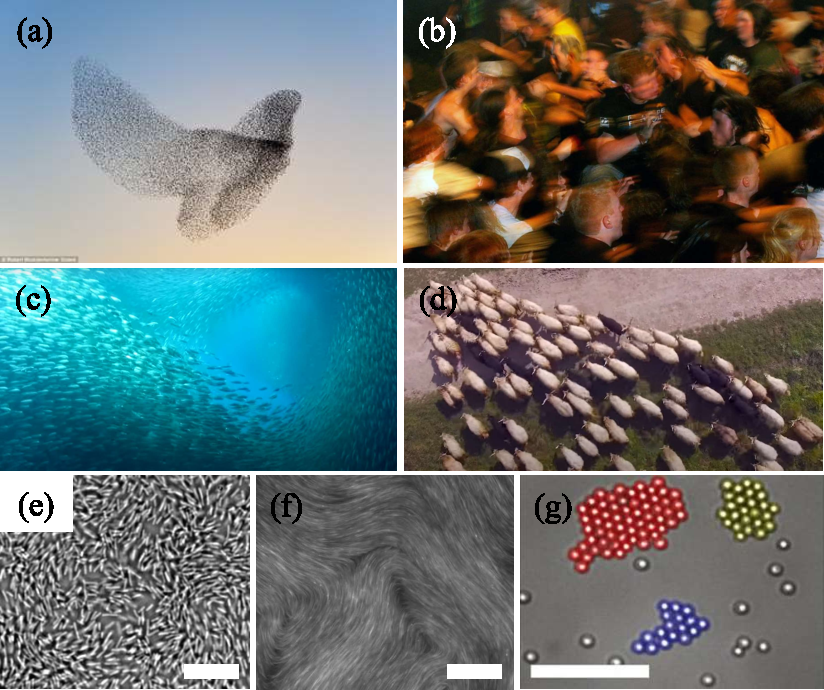
\includegraphics[width=5.5 in]{Figs/1-Intro/1.pdf}
	%select pdftexify command to run jpg or pdf files
	\end{center}
	\caption[Figure 1.1: ]
	{
	\textbf{Examples of living matters and active fluids.}
  (a) Flocking birds, (b) people in a mosh pit at heavy metal converts, (c) schooling fish, (d) herding sheeps, (e) swarming bacteria (f) microtubule and (g) clustering active Janus particles.
  Scalebars in (e) and (g) are 10 \textmu m. Scalebar in (f) is 200 \textmu m. Images courtesy of Robert Wolstenhome (a), Ulrike Biets (b) \cite{Silverberg2013}, biographic (c, d), DeCamp (f) \cite{DeCamp2015} and Palacci (g) \cite{Palacci2013}.
	}
	\label{fig:1-1}
\end{figure}

\section{Novel Properties}
\label{emergent-properties}
Active fluids exhibit novel properties such as reduced viscosity and enhanced diffusion  \cite{Ramaswamy2010}. The reduced viscosity is induced by the force excerted by the swimming mechanisms of the active agents, such as bacteria and algae \cite{Saintillan2018}. And the enhanced diffusion is attributed to the interaction - steric collision or hydrodynamic perturbation - between tracer particles and swimmers
\cite{Wu2000, Peng2016, Caspi2000, Morozov2014, Patteson2016, Leptos2009,
 Yang2016, Valeriani2011, Kurtuldu2011}.
In this section, the existing works regarding rheology and diffusion in active fluids are reviewed, and motivations for investigating the rheology of bacterial suspensions under confinement (Chap.~\ref{rheology-of-bacterial-suspensions-under-confinement}) will be discussed.


\subsection{Rheology}
\label{sec:rheology}
Viscosity of a fluid can be understood as its resistence to flow. When flowing, fluid elements move relative to others, resulting in energy dissipation due to friction. The more energy is required, the more "viscous" the fluid is known to be. A suspension
of passive particles is always more viscous than its suspending fluid, a fact that was first formulated by Einstein in 1906 \cite{Einstein1906}. Recently, the study of active fluids revealed that active particles modify the viscosity of their suspending fluids in a different and interesting way.

In 2004, Hatwalne et al. predicted that micro-swimmers, depending on their self-propelling mechanisms, can modify the suspension viscosity in different ways \cite{Hatwalne2004}. Most common micro-swimmers, such as unicellular microorganisms, can be classified into two types: pushers and pullers, based on the far field flow they generate. Fig.~\ref{fig:1-2}b illustrates the most common pushers and pullers in nature: bacterium and algae. If one puts a elongated rod-like bacterium in a simple shear flow, as illustrated in Fig.~\ref{fig:1-2}a, the preferred orientation of the bacterium is along the extensile flow \cite{Forster1974}. Such an orientation makes the flow generate by the swimming bacterium coincide with the imposed shear flow, and thus compensating the viscous dissipation of energy, which effectively reduces the viscosity. In contrast, in the case of puller swimmers, such an orientation makes opposites the directions of swimming induced flow and imposed shear flow, which enhances the visocity.

Their prediction was confirmed by numerical solutions of the theory \cite{Cates2008, Giomi2010} and experiments \cite{Sokolov2009, Gachelin2013, Lopez2015}. Cates et al. reached at the same conclusions as Hatwalne et al. did: while contractile gels exhibit a divergence of apparent viscosity, extensile gels show a zero-viscosity phase. Giomi et al., on top of these results, emphasized the important role of particle shape. They showed, in their numerical study, an rheological equivalence between rod-like pusher swimmers and disk-like puller swimmers (see Fig.~\ref{fig:1-2}c). In particular, they predicted a thickening effect of spherical puller swimmers (corresponds to the 0 shape parameter in Fig.~\ref{fig:1-2}c). This prediction was later on challenged by another theory in the framework of swim stress, which predicts a viscosity reduction of a spherical pusher swimmer suspension
\cite{Takatori2017}. Due to the difficulty of synthesizing large amount of artificial swimmers, this debate has not been resolved yet. However, with the rapid development of synthesizing techniques \cite{Palacci2013, Bricard2013}, it is getting more promising that we will resolve it, and formulate a more complete understanding on how active swimmers modify the rheology.

Experimental confirmation of these predictions posed challenges on traditional rheometries due to the tiny shear stress that is required to be measured. As a result, new rheometries are needed \cite{Marchetti2015}. In 2009, Sokolov and Aranson came up with an innovative way of measuring the such tiny stress \cite{Sokolov2009}. By moving a probe in a suspension of \textit{Bacillus subtilis} bacteria, a pusher type swimmer, they generated a large vortex. By studying the decay of the vortex, they got a measure of the viscosity. For the first time, they experimentally confirmed that pusher swimmers reduced the viscosity (see their results in Fig.~\ref{fig:1-2}d). In 2013, Gachelin et al. adopted a microfluidic viscometer to measure the viscosity of suspensions of \textit{Escherichia coli} bacteria, another pusher type swimmer \cite{Gachelin2013}. They confirmed again the viscosity reduction. A more remarkable finding is the non-newtonian behavior: the viscosity was reduced at low shear rate, but was enhanced at high shear rate. This observation suggested that it is the competation between bacterium intrinsic shear rate and the impose flow shear rate that determines how the viscosity is modified. In 2015, Lopez et al. published arguably the most important experimental work on the rheology of active fluids, which showed that the apparent viscosity of an \textit{E. coli} suspension can be reduced to zero if the swimming activity is sufficiently high \cite{Lopez2015}. The authors modified an old-fashioned Couette concentric cylinders, where the outer cylinder was set to rotate at a fixed rate and the torque on the inner cylinder was measured. The high sensitivity was achieved by using a string that was highly sensitive to torque to hang the inner cylinder, so that a stress, as small as that generated by bacterial suspensions, can be detected (see their rheometer and results in Fig.~\ref{fig:1-2}e-f). The authors termed their zero-viscosity suspensions ``superfluids''.

Despite the great progress on the rheology of active fluids made so far, their remained complexity that are not readily understood. Confinement, or more generally boundary conditions or geometry, is one of the leading factors that contribute to this complexity. The behavior of active particles can be altered greatly by confinement. In 2005, Voituriez et al. showed theoretically that a spontaneous flow transition from a homogeneous immobile state could happen in active polar gel under confinement \cite{Voituriez2005}. Such spontaneous flow transition was confirmed in both numerical and experimental studies \cite{Ravnik2013, Wioland2016, Wu2017}. The complexity introduced by geometry was also manifested by the experiments where single bacterial vortex was stabilized by confinement \cite{Woodhouse2012, Wioland2013, Lushi2014} and where asymmetric gears were powered by swimming bacteria
\cite{Sokolov2010, Hamby2018}. The effect of confinement on the rheology of active fluids was first studied theoretically based a kinetic theory \cite{Alonso-Matilla2016} and a generalized Navier-Stokes model \cite{Slomka2017}. In this thesis, I will present the first experimental study on active fluid rheology using bacterial suspensions
(Chap.~\ref{rheology-of-bacterial-suspensions-under-confinement}). The fact that our experimental results agreed with neither theory manifested the complexity and the lack of understanding of active fluids. Together with the experimental results, we provided a heuristic model that qualitatively captured the rheological properties and hope to stimulate further theoretical studies on this matter.

\begin{figure}[!htbp]
	\begin{center}
	\includegraphics[width=5.5 in]{Figs/1-Intro/2.pdf}
	%select pdftexify command to run jpg or pdf files
	\end{center}
	\caption[Figure 1.2: ]
	{
	\textbf{Rheology of active fluids.}
	(a) The preferred orientation of the bacterium is along the extensile flow.
	(b) The most common pushers and pullers in nature: bacterium and algae, and their corresponding far field flow.
	(c) Rheological effect phase diagram of swimmer shape and swimming mechanism.
	(d) Non-Newtonian behavior of \textit{E. coli} suspensions.
	(e) Stress response of \textit{E. coli} suspensions in a modified Couette concentric cylinder rheometer.
	(f) Viscosity of \textit{E. coli} suspensions at various volume fractions.
	Image courtesy of Marchetti (a, b) \cite{Marchetti2015}, Giomi (c) \cite{Giomi2010}, Gachelin (d) \cite{Gachelin2013} and Lopez (e, f) \cite{Lopez2015}.
	}
	\label{fig:1-2}
\end{figure}


\subsection{Diffusion}
\label{sec:diffusion}
The diffusion of passive particles in active fluids, such as nutrients and signaling molecules, are significantly enhanced. Such enhancement has been shown to have great biological and ecological importance \cite{Wu2000, Kurtuldu2011, Morozov2014}, as well as to provide a useful tool of probing novel properties of active fluids \cite{Squires2010}. Unlike the study of rheology, which was initiated by theoretical prediction, the study of enhanced diffusion started from an experiment.

In 2000, Wu and Libchaber studied the diffusion of spherical polystyrene particles in a bath of actively swimming \textit{E. coli} \cite{Wu2000} (see Fig.~\ref{fig:1-3}a for their experimental system). They characterized the diffusion of the tracer particles by measuring their means squared displacement (MSD) (see Fig.~\ref{fig:1-3}b for typical MSD data), and reported two findings: 1) the MSD exhibits a superdiffusive regime at short time, which is followed by a diffusive regime at longer time; 2) the effective temperature, backed up from effective diffusion coefficient using Stokes-Einstein equation, is several order of magnitude larger than room temperature. Their qualitative findings were confirmed by computational \cite{Underhill2008, Lin2011}, theoretical \cite{Golestanian2009} and other experimental studies
\cite{Chen2007, Leptos2009, Mino2011, Kurtuldu2011, Patteson2016}. A remarkable progress towards quantitative understanding was made by Mino et al., who experimentally identified that the enhancement of diffusivity is proportional to the "activity flux" (defined as concentration multiplied by the mean velocity of swimmers). This model was further developed to capture the experimental result more accurately and to account for more complex conditions \cite{Mino2013, Kasyap2014, Morozov2014}.

Although a lot of progress has been made on understanding diffusion isotropic particles (spheres) in an active bath, how anisotropic particles diffuse remained largely unexplored. Yet, the diffusion of anisotropic particles has both fundamental and application significance. On the one hand, it was shown that the Brownian motion (i.e. in a passive bath) of anisotropic particles exhibited a subtle interplay between orientational and translational motions \cite{Han2006}. Previous studies preferred to consider an active bath equivalent to a high temperature passive bath \cite{Wu2000}, and it was shown to be a good equivalence for isotropic particles. A fundamentally interesting question to ask is: does active bath also alters the interplay between orientational and translational motions? The answer is yes, and we will see that this interplay is specific to swimming mechanisms. On the other hand, few particles or molecules in nature are perfectly isotropic. Generalizing the enhanced diffusion to anisotropic particles will have significant impact on applying this knowledge on real world problems. In 2016, Peng et al. studied the diffusion of polystyrene ellipsoids in a quasi-2D free-standing soap film of \textit{E. coli} bath (see setup schematic in Fig.~\ref{fig:1-3}c) \cite{Peng2016}. In contrast to the pure Brownian motion, where ellipsoids preferred to diffuse along their major axes \cite{Han2006}, they found that an active bath forced
the ellipsoids to move primarily along the minor axes (see Fig.~\ref{fig:1-3}d-e for a comparison). This phenomenon was explained by considering the far-field dipole flow of a single \textit{E. coli} bacterium. An interesting prediction naturally arises: in a bath of puller swimmers, whose far-field flow is opposite to that of pushers, the diffusion of ellisoidal tracers should be primarily along the major axes. This prediction was later on proved experimentally by Yang et al. \cite{Yang2016} in a green algae \textit{C. reinhardtii} bath and I was involved in this work. Due to the fact that my contribution was relatively small to this work, I will not provide more details about it in my thesis. However, readers interested are encouraged to find out more in our original paper \cite{Yang2016}.

\begin{figure}[!htbp]
	\begin{center}
	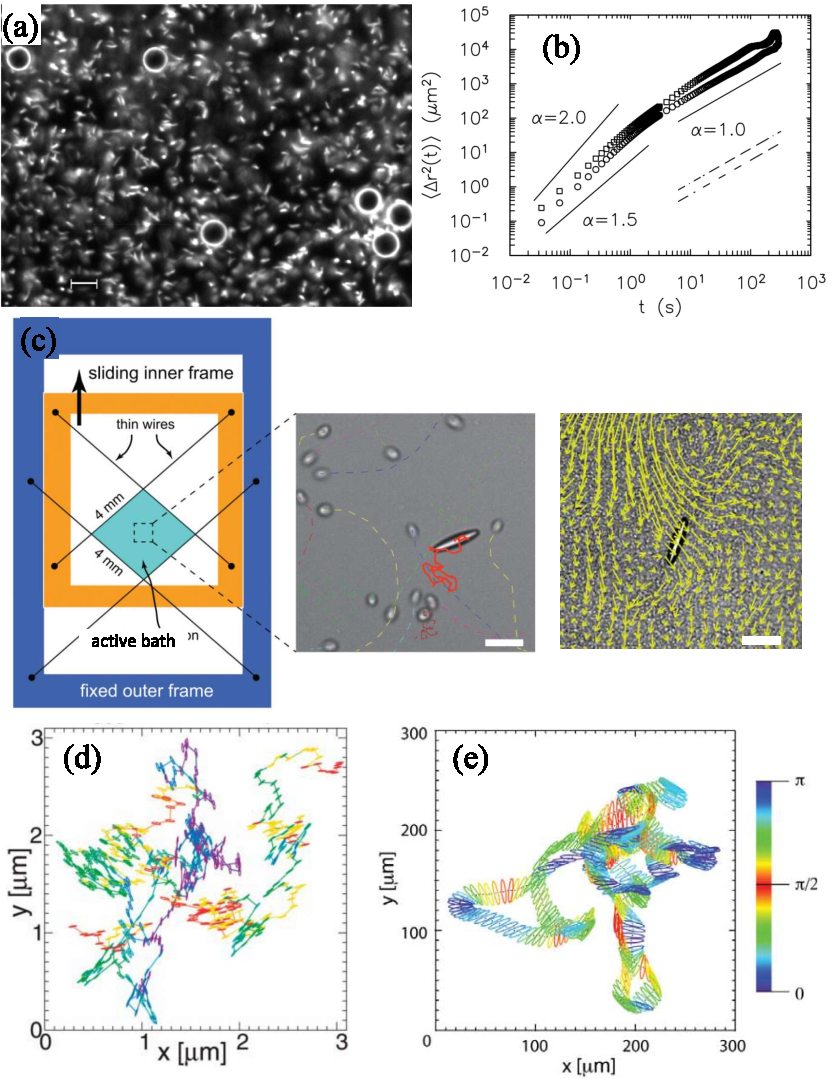
\includegraphics[width=5.5 in]{Figs/1-Intro/3.pdf}
	%select pdftexify command to run jpg or pdf files
	\end{center}
	\caption[Figure 1.3:]
	{
	\textbf{Diffusion of passive tracers in an active bath.}
	(a) 10 \textmu m diameter PS particles suspended in a bath of \text{E. coli}
	(b) Mean squared displacement (MSD) of tracer paticles as a function of lag time.
	(c) Free-standing film setup adopted by Peng et al. and Yang et al. (left)\cite{Peng2016, Yang2016}. A microscopic image of ellipsoidal PS particle suspending in \textit{C. reinhardtii} (middle) and \textit{E. coli} (right) baths. Scale bar: 20 \textmu m.
	(d) and (e) present both the translational and orientational trajectories of ellipsoids diffusion in water and \textit{E. coli} bath, respectively.
	Image courtesy Wu (a, b) \cite{Wu2000}, Yang (c) \cite{Yang2016}, Han (d) \cite{Han2006} and Peng (e) \cite{Peng2016}.
	}
	\label{fig:1-3}
\end{figure}



\section{Collective Motion and Giant Number Fluctuations}
Collective motion is defined as an emergent directed movement in a large number of animals or particles, which are capable of moving on their own.




\subsection{Collective Motion}
The research on collective phenomena dates back to the 1980s, when flocking birds, schooling fish, herding beasts and even human crowds (Fig.~\ref{fig:1-1}a-d) were regarded as an orientationally ordered phase of living matter, in analogy with ferromagnetic spins
\cite{Reynolds1987, Vicsek1995, Narayan2007, Ward2008, Ballerini2008, Silverberg2013}. This idea has since evoked enormous research interest on this seemingly universal animal behavior and its consequences. In this section, we first review recent progresses on understanding the collective phenomena in various living systems and motivate our research on "imaging the emergence of active turbulence"
(detailed in Chap.~\ref{the-emergence-of-active-turbulence}). Then, I will switch to an important consequence of the collective phenomena: giant number fluctuations, where I will motivate our research on "giant number fluctuations in 3-dimensional bacterial suspensions" (detailed in Chap.~\ref{giant-number-fluctuations-in-3-dimensional-space}).

Besides macroscopic systems mentioned above, smaller and more laboratory accessible model systems have joined this family and have been studied extensively. As examples, actin filaments and bacteria exhibit turbulence-like swirling patterns, and synthetic active colloids form dynamic clusters (Fig.~\ref{fig:1-1}e-g)
\cite{Dunkel2013, Wensink2012, Buttinoni2013, Palacci2013, Sanchez2012, Schaller2010, Sokolov2007}. As of today, these universal patterns can be qualitatively reproduced by simple models with collision rules and noise. And quantitative description is developing with more observations available, which is bound to have impactful applications, including understanding the reaction of panic crowd and predicting the migration of fish schools
\cite{Vicsek2012}.

Basic models Vicske model, continuum

Phase transitions

To test the prediction of the kinetic theory by Saintillan and Shelly, we perform experiment
\subsection{Giant Number Fluctuations}
Large scale inhomogeneity

% \chapter{Experimental Background}
\label{experimental_background}
%%%%%%%%%%%%%%%%%%%%%%%%%%%%%%%%%%%%%%%%%%%%%%%%%%%%%


\section{Confocal Laser Scanning Microscopy}
\label{Experiment_CLSM}
%%%%%%%%%%%%%%%%%%%%%%%%%%%%%%%%%%%%%%%%%%%%%%%%%%%%%
%%%%%%%%%%%%%%%%%%%%%%%%%%%%%%%%%%%%%%%%%%%%%%%%%%%%%
%If you wish to place the figure near, allow more positioning options, for instance by [htbp] (here, top, bottom, page). Use a ! symbol to remove further restrictions.
\begin{figure}[!htbp]
	\begin{center}
	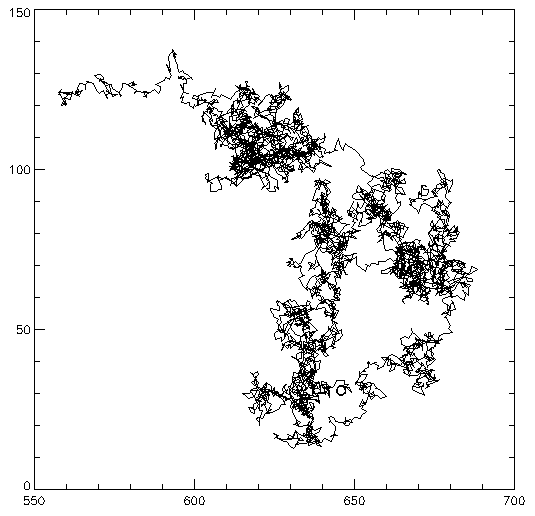
\includegraphics[width=4 in]{Figs/2-Exp/tracks.png}
	%select pdftexify command to run jpg or pdf files
	\end{center}
	\caption[]
	{

	}
	\label{}
\end{figure}
%%%%%%%%%%%%%%%%%%%%%%%%%%%%%%%%%%%%%%%%%%%%%%%%%%%%%


% Results
\chapter[Rheology under Confinement]{Rheology of Bacterial Suspensions under Confinement\footnote[1]{
Reproduced in part with permission from (Zhengyang Liu, Kechun Zhang and Xiang Cheng, ``Rheology of bacterial suspensions under confinement'', \textit{Rheologica Acta}, Springer).
}}

\label{rheology-of-bacterial-suspensions-under-confinement}
%%%%%%%%%%%%%%%%%%%%%%%%%%%%%%%%%%%%%%%%%%%%%%%%%%%%%

\section{Introduction}
An active fluid is a suspension of self-propelled particles in fluid media with examples including a wide range of biological and physical systems ranging from swimming microorganisms
\cite{Schwarz-Linek2016} to suspensions of synthetic colloidal swimmers \cite{Palacci2010, Palacci2013, Bricard2013} and to ATP-driven cytoskeletons \cite{Sanchez2012, Schaller2010}.
With the ability of converting ambient or internal free energy to mechanical work at microscopic scales, active fluids can maintain a nonequilibrium steady state with uniform free energy input and display features drastically different from those of passive colloidal suspensions \cite{Koch2011, Marchetti2013, Bechinger2016, Elgeti2015, Saintillan2015}.
Many nonequilibrium properties of active fluids such as the emergence of collective motions \cite{Sokolov2012, Wensink2012, Cisneros2011, Guo2018}, giant number fluctuations \cite{Narayan2007, Zhang2010},
and enhanced diffusion of passive particles \cite{Wu2000, Mino2013, Morozov2014, Peng2016, Yang2016} have been extensively studied in recent years. Among all these novel properties, the rheological response of active fluids presents arguably the most surprising phenomena, challenging our understanding of the flow of complex fluids \cite{Saintillan2018}. By measuring the decay of large vortices and the torque on a rotating probe, Sokolov and Aranson first experimentally showed that the viscosity of bacterial suspensions in a freestanding film can reduce by a factor of seven compared with the suspending fluid without bacteria \cite{Sokolov2009}. Gachelin and co-workers used a Y-shaped microfluidic channel---a technique we will adopt below in our study---to measure the viscosity of bulk bacterial suspensions \cite{Gachelin2013}. They showed that the viscosity of bacterial suspensions can be significantly lower than that of the suspending fluid.
More recently, measurements by Lopez et al. using a conventional bulk rotational Couette rheometer demonstrated zero or even a negative apparent viscosity in bulk bacterial suspensions at low shear rates \cite{Lopez2015}. In contrast to pusher swimmers such as bacteria, suspensions of algae, an example of puller swimmers, show a noticeable viscosity enhancement compared with suspensions of immobile algae at the same concentrations \cite{Rafai2010}.

Several mechanisms have been proposed to explain the unusual rheology of active fluids (see Ref.~\cite{Saintillan2018} and references therein). The most widely circulated theory considers
the coupling between the orientation of elongated bacteria modified by external shear and the intrinsic force dipoles exerted by bacteria on the suspending fluid. Orientated along the extensional quadrant of an imposed shear flow, a bacterium exerts a force dipole on the fluid, which induces a disturbance flow opposite to that induced by a passive elongated particle of the same shape.
Such an effect, first explained by Hatwalne et al. \cite{Hatwalne2004}, leads to a reduction of the resistance of pusher suspensions to shear and the decrease of suspension viscosity. Incorporating further orientational dynamics of bacteria, continuum kinetic theories have been constructed based on the above picture, which quantitatively explained the rheology of dilute bacterial suspensions
\cite{Haines2009, Saintillan2010, Ryan2011, Moradi2015, Alonso-Matilla2016, Bechtel2017}.
Hydrodynamic models have also been developed along a similar line \cite{Cates2008, Giomi2010, Somka2017}, which successfully predicted the existence of bacterial superfluids with a zero apparent viscosity \cite{Marchetti2015}.
A second viscosity-reduction mechanism has recently been proposed by Takatori and Brady \cite{Takatori2014a, Takatori2014b, Takatori2017}. They considered the coupling between the shear flow and the swimming and rotational motion of active particles, which gives rise to an anisotropic active diffusivity in analogy of Taylor dispersion. The resulting diffusive stress stretches the fluid along the extensional direction of shear, similar to the effect of the force dipole induced by individual pusher swimmers, which leads to viscosity reduction even for spherical swimmers.
Lastly, experiments on suspensions of bacteria and microtubules suggested that elongated active particles align near a system boundary and form a smectic layer along confining walls in self-driven flows \cite{Wioland2016, Wu2017, Lushi2014}.
This boundary layer collectively propels the fluid in the bulk and results in a selfsustained directional flow with a zero or negative apparent
viscosity.

While the rheology of bulk bacterial suspensions has been measured \cite{Gachelin2013, Lopez2015}, the effect of confinement on the rheology of bacterial suspensions has not been explored experimentally. The study of the rheology of confined bacterial suspensions is important from both fundamental and practical perspectives. First, the study shall provide crucial information for verifying different models. In particular,
the boundary-layer mechanism suggests that the unusual rheology of active fluids originates from the boundary and, therefore, should strongly depend on system sizes. In comparison, both the kinetic theory and the diffusive stretching theory apply for bulk suspensions. Confinement
may modify the rheology of active fluids in these theories indirectly via effects such as the change of particle orientations and density distributions near confining walls \cite{Alonso-Matilla2016}
Second, various interesting collective dynamics including spontaneous directional flows \cite{Wioland2016, Wu2017, Lushi2014} and stable bacterial vortices \cite{Lushi2014, Wioland2013, Wioland2016b} have been found in confined active fluids. The consequence of
these new phases on the rheology of active fluids is still unclear.
Finally, confinement is frequently encountered in natural context of microbial systems, e.g. sperm cells in reproductive tracts and microorganisms in soil and biofilms \cite{Foissner1998, Or2007}. Thus, the study on the rheology of
confined bacterial suspensions will also help to understand bacterial transport in confined geometries.

Here, using \textit{Escherichia coli} (\textit{E. coli}) as our model active swimmers, we experimentally study the rheology of active fluids in microfluidic channels under different degrees of confinement.
Our study reveals a strong confinement effect on dilute bacterial suspensions: the apparent viscosity of suspensions reduces by a factor of three when the confinement scale decreases from 60 down to 25 $\mu$m. We demonstrate that the effect of confinement is directly linked to the motility of bacteria. Furthermore, we also probe the microscopic dynamics of sheared bacterial suspensions such as the velocity profiles of
suspension flows and the variation of bacterial density within confined channels. These microscopic measurements allow us to construct a simple model based on the boundary-layer mechanism, which qualitatively explains the experimental observations.
Thus, our study provides not only systematic experimental results on the rheology of confined bacterial suspensions but also evidence on the effect of the boundary layer on the rheology of active fluids.

\begin{figure}[!ht]
	\begin{center}
	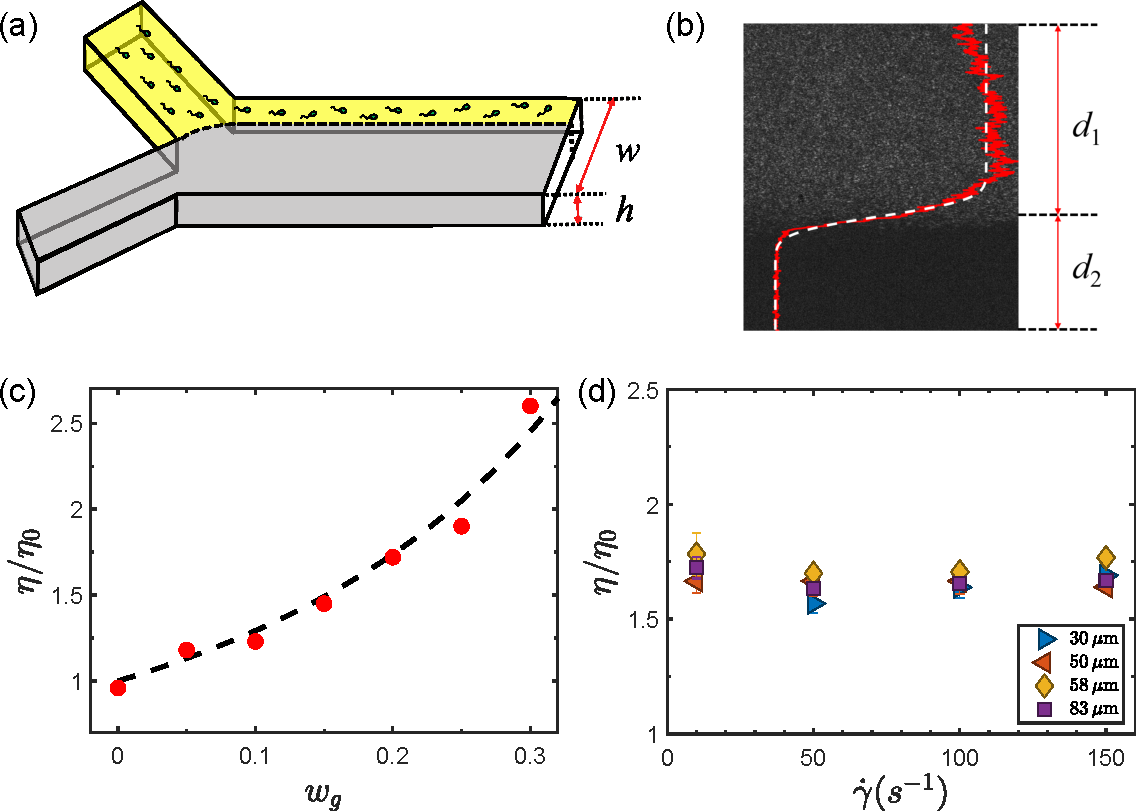
\includegraphics[width=5.5 in]{Figs/3-Rheo/1.pdf}
	\end{center}
	\caption[Microfluidic viscometer.]
	{
	\textbf{Microfluidic viscometer.}
  (a) Schematic of the Y-shaped microfluidic channel.
  (b) Image of two fluids in the channel. The upper region is a bacterial suspension with width $d_1$, whereas the lower region is the suspending fluid with width $d_2$. The red line shows the intensity profile across the channel. The white dashed line is the error function fitting.
  (c) Viscosity of water-glycerol mixtures at different glycerol weight
  fractions, $w_g$. Shear rate $\dot\gamma = 100$ s$^{-1}$. The dashed line is the literature value.
  (d) Viscosity of a water-glycerol mixture (20 w\% glycerol) as a function of shear rates at different channel heights $h$. The literature value of the viscosity of the mixture is 1.74 mPa s at 20 °C. $h$ is indicated in the figure.
	}
	\label{fig:3-viscometer}
\end{figure}

\section{Methods}
\subsection{E. coli suspensions}
In our experiments, we use a fluorescently tagged \textit{E. coli} K-12 strain (BW25113) as our microswimmers, which carry the
PKK PdnaA-GFP plasmid. These fluorescent cells allow us to image suspension flows with fluorescence and confocal microscopy. To prepare a motile E. coli suspension, bacteria are first cultured overnight at 37 °C in a terrific broth (TB) culture medium (tryptone 11.8 g/L, yeast extract 23.6 g/L, and glycerol 4 ml/L) supplemented with a 0.1\% (v/v) selective antibiotic (ampicillin 100 mg/L). A small volume of the overnight culture is then diluted in a fresh TB culture medium (1:100) and grown at 30 °C in a shaker at 220 rpm for 6.5 h. The culture is finally washed with a motility buffer via centrifuging (5 min, 800 g) and set to a desired concentration of $n = 1.6 \times 10^{10}$ cells/ml. At this dilute concentration, bacteria do not show strong collective swarming \cite{Guo2018}. For an isolated wild-type \textit{E. coli}, it executes the so-called run-andtumble motion \cite{Berg2004}. In the ``run'' phase, the cell is propelled forward by a flagellar bundle at a constant speed $v \approx 22$ $\mu$m/s. The straight ``run'' is punctuated by a sudden and rapid ``tumble'' at a rate $f$ on the order of 1 Hz, which randomizes the orientation of the cell. The run length of bacteria
is thus given by $L = v/f$. For the wild-type bacteria, we have $L = 33.1 \pm 8.1$ $\mu$m.

For control experiments, we also culture a mutant strain of \textit{E. coli}, which exhibits only tumbling motions without run. The tumbler strain we use is RP1616 ($\Delta cheZ$), which is a derivative from RP437, a strain commonly used in chemotaxis study \cite{Parkinson1978} (Parkinson 1978). Phospho-CheYand CheZ are the two primary emzymatic complexes governing bacterial chemotactic behaviors. Phospho-CheY enhances the clockwise rotation of the flagellar motors that enables the tumbling of bacteria. CheZ promotes the dephosphorylation rate of phospho-CheY to make the bacteria stop tumbling and transition into the ``run'' phase. Thus, the function of CheZ ensures that bacterial tumbling is short and the locomotor responses to changes in chemicals are rapid. By knocking out $cheZ$, we slow down the dephosphorylation rate of phospho-CheY, which leads to the accumulation of phospho-CheY in bacteria. The excessive phospho-CheY makes the bacteria keep tumbling instead of performing a run-and-tumble motion. The culturing procedure of tumblers is the same as the one for the swimmers described above. Lastly, we test the rheology of the dead bacteria as control. Bacteria are neutralized by adding 10 mM sodium azide in the suspensions.

\subsection{Microfluidic viscometer}
We use a microfluidic viscometer for viscosity measurement. The same technique has been used in studying the rheology of bulk bacterial suspensions \cite{Gachelin2013}. As sketched
in Fig.~\ref{fig:3-viscometer}a, the viscometer consists of a symmetric Y-shape microfluidic channel with height $h$ and width $w$ in the main channel. In order to investigate the effect of confinement, we
fabricate channels of different $h$ ranging from 25 up to 128 $\mu$m, whereas w is fixed at 600 $\mu$m. The two side branches have the same height $h$ but half of the width of the main
channel $w/2$. Under these conditions, the flow in the main channel satisfies the Hele-Shaw approximation (Lamb 1932), where shear gradients along the height direction ($y$) dominate the flow. We define a coordinate system in the main channel as follows: $x$ is along the flow direction, $y$ is along the height direction with dominant shear gradients, and $z$ is the vorticity direction along the width of the channel.
The origin of the coordinate is set at the center of the channel with $y \in [-h/2, h/2]$ and $z \in [-w/2, w/2]$.

In a typical experiment, we inject a bacterial suspension of unknown viscosity and the suspending fluid of known viscosity into the microfluidic channel through the two side branches separately at the same flow rate using a syringe pump (Harvard Apparatus, 11 Elite) and two 100-$\mu$l syringes (Scientific Glass Equipment). The interface between the two fluids stabilizes downstream of the merging point of the two branches in the main channel with the width of the two fluids at $d_1$ and $d_2$, respectively.
Since the bacteria constantly migrate across the interface from the suspension into the suspending fluid, the interface gradually smooths out along the flow. We measure $d_1$ and $d_2$ at the position where the interface is stable and sharp, typically 500 to 1000 $\mu$m downstream of the merging point (Fig.~\ref{fig:3-viscometer}b).
It can be shown that the viscosity ratio of the two miscible fluids in the channel, $\eta_1/\eta_2$, is equal to the width ratio $d_1/d_2$ \cite{Guillot2006, Nghe2010}. We test the accuracy of the viscometer at different h by measuring the viscosity of water-glycerol mixtures.
The results from the microfluidic viscometer quantitatively agree with the known viscosity of the mixtures and are independent of the channel height in the range of our experiments (Fig.~\ref{fig:3-viscometer}c and d).

In this study, we take the nominal wall shear rate $\dot\gamma\equiv 6Q/(d_1h^2)$ as a characteristic shear rate on bacterial suspensions, where $Q$ is the control flow rate. The formula is exact when
the velocity profiles of suspensions are parabolic following the Hagen-Poiseuille law. The average of the magnitude of shear rates in the channel is then $\dot\gamma/2$. For non-parabolic profiles, the formula can be simply treated as a definition of the characteristic shear rate in the channel. For each channel height $h$, we decrease $Q$ from 100 to 1 $\mu$l/h to examine the
rheological response of bacterial suspensions at different $\dot\gamma$. At an even lower $Q$, the interface between the suspensions and the suspending fluid becomes unstable and displays nonplanar
longitudinal variations, which prevents us from measuring the width ratio of the two fluids accurately. Such instability may indicate nonzero normal stress differences in bacterial suspensions \cite{Hinch1992, Brady2002, Saintillan2010}.

\subsection{Image acquisition and analysis}
Florescence microscopy is used to take movies of the microfluidic flows at the center of the channel at $y = 0$. Movies are acquired at 30 frames per second (fps) with a sCMOS camera (Andor, Zyla) through an inverted microscope (Nikon, Ti-E) using a 10X objective. Raw images are first processed by a variance filter to enhance the contrast between bacterial suspensions and the suspending fluid
(Fig.~\ref{fig:3-viscometer}b). For each image, we calculate the sum of the pixelintensity in each row and then obtain an intensity profile of the image along the width of the channel ($z$) (Fig.~\ref{fig:3-viscometer}b, red curve). By fitting the intensity profile with an error function (Fig.~\ref{fig:3-viscometer}b, white curve), we identify the position of the interface between the two fluids as the reflection point of the error function. This image analysis routine is implemented using a custom Matlab program.

To obtain the flow profiles of suspensions at different $h$ and $\dot\gamma$, we add fluorescent polystyrene (PS) colloids of 1 $\mu$m in diameter into bacterial suspensions. At 0.001 v\% in the final mixture, the concentration of PS particles is so low that the presence of the particles should not affect the flow of bacterial suspensions. We use fast confocal microscopy to measure suspension flows at different heights above the bottom wall of microfluidic channels away from the side walls. At each height, a movie of 10–20 s is taken at 100 fps using a 60X objective. The velocity of fluid flows at a certain $y$, $V(y)$, is extracted by tracking the motion of colloids in the imaging plane using particle tracking velocimetry (PTV). In addition, we also measure the average velocity of bacteria, $V_{bac}(y)$, via particle imaging velocimetry (PIV), where bacteria, instead of colloids, are used as tracer particles. Both the velocity profile of fluid flows and the velocity profile of bacteria along y can then be compiled from a series of measurements at different heights. The measurements on $V(y)$ and $V_{bac}(y)$ yield not only the flow profile of suspensions but also the relative motions between bacteria and the suspending fluid. The disturbance flow $V_d(y)$ defined below can be obtained as $V_d(y) = V(y) - V_{bac}(y)$.

The number of bacteria at each height can also be estimated from these movies through direct counting, which allows us to calculate 2D bacterial density $n$.

\begin{figure}[!ht]
	\begin{center}
	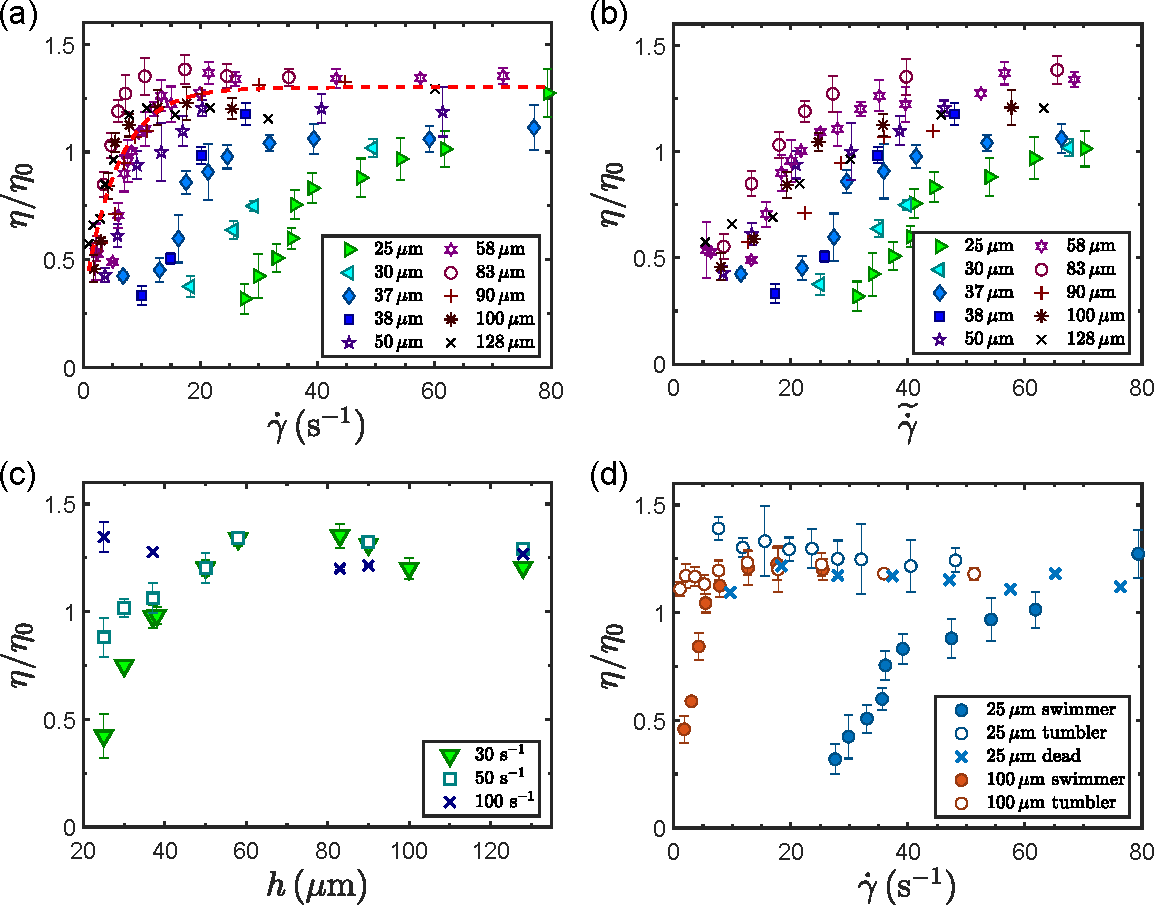
\includegraphics[width=5.5 in]{Figs/3-Rheo/2.pdf}
	\end{center}
	\caption[Viscosity of bacterial suspensions under different degree of confinement]
	{
	\textbf{Viscosity of bacterial suspensions under different degree of confinement.}
  (a) $\eta/\eta_0$ as a function of shear rates, $\dot\gamma$ , in channels of different heights, $h$. $h$ is indicated in the figure. The dashed line is a fitting for the bulk samples with $\eta/\eta_0=1.3-\exp(-0.24\dot\gamma)$. (b) $\eta/\eta_0$ as a function of dimensionless shear rates, $\tilde{\dot\gamma}$, in channels of different $h$. $\tilde{\dot\gamma}\equiv\dot\gamma h/v$, where bacterial swimming speed $v = 22$ $\mu$m/s.
  (c) $\eta/\eta_0$ as a function of $h$ at different $\dot\gamma$, which are indicated in the figure.
  (d) $\eta/\eta_0$ of suspensions of active swimmers, tumblers, and dead bacteria. Two different heights $h = 25$ $\mu$m and 100 $\mu$m are used.
	}
	\label{fig:3-rheology}
\end{figure}

\section{Results}
\subsection{Confinement effect}
Fig.~\ref{fig:3-rheology}a shows the relative viscosity of bacterial suspensions, $\eta/\eta_0$, as a function of shear rates for channels of different heights. Here, $\eta$ is the viscosity of bacterial suspensions and $\eta_0$ is the viscosity of the suspending fluid. For channels with $h > 60$ $\mu$m, the flow curves of different heights collapse into a master curve, giving the rheological response of bulk bacterial suspensions. At low shear rates, suspensions show strong shear thickening. When $\dot\gamma < 10$ s$^{-1}$, the viscosity of bacterial suspensions is below that of the suspending fluid, a defining feature of the rheology of pusher suspensions. At the lowest
shear rate of our experiments $\dot\gamma=1$ s$^{-1}$ , the viscosity is about half of the viscosity of the suspending fluid, quantitatively agreeing with previous experiments \cite{Gachelin2013}. However, for channels with $h < 60$ $\mu$m, the flow curves separate from each other at low shear rates, indicating a strong confinement effect at a small $h$. At high shear rates, the relative viscosity at different heights approaches to a plateau independent of $h$. This absence of the confinement effect at high shear rates suggests that the effect is linked to bacterial motility. In the limit of high shear rates, the active stress arising from the hydrodynamic stresslet and the diffusive stress is negligible compared with the passive stress induced by the rigid elongated body of \textit{E. coli} on the fluid \cite{Takatori2017, Saintillan2018}. Thus, the viscosity of active suspensions in
the limit of high shear rates should be the same as that of suspensions of passive elongated particles of the same shape, which does not show an obvious confinement effect. We also observe weak shear thinning in this regime, presumably arising from the shear-induced alignment of elongated particles \cite{Egres2006}. The degree of shear thinning, however, is weaker than that reported in the previous study \cite{Gachelin2013}.

We have attempted to rescale the relative viscosity by normalizing the shear rate by the characteristic run-time of
bacteria, which determines the diffusive stress of active particles \cite{Takatori2017}. The dimensionless shear rate $\tilde{\dot\gamma}$ is defined as $\tilde{\dot\gamma}\equiv \dot\gamma / f$, where $f$ is the tumbling frequency of bacteria. For bulk samples with $h > 60$ $\mu$m, $f \approx 0.5$ Hz is an intrinsic property of bacteria and therefore a constant. Since the relative viscosity has already collapsed together when plotting against $\dot\gamma$, adding a constant prefactor should not change the quality of data collapsing. For confined samples, the tumbling frequency of bacteria is determined by the system size. In a simple picture, $f$ should be replaced by $v/h$. Although different data sets show better collapse when plotted against $\tilde{\dot\gamma}$, they are still well separated (Fig.~\ref{fig:3-rheology}b). The result suggests that other factor(s) in addition
to the reorientation of bacteria need to be considered in order to fully interpret our experiments on strongly confined samples.

The confinement effect is even better illustrated in Fig.~\ref{fig:3-rheology}c, where the relative viscosity of bacterial suspensions as a function of channel heights is directly plotted at three different shear rates. At the lowest shear rate, the viscosity increases by a factor of three when the confinement length increases from 25 to 60 $\mu$m. Above $h \approx 60$ $\mu$m comparable with the run length of bacteria, the viscosity plateaus and becomes
independent of $h$. At the moderate shear rate, the increasing trend is less pronounced. At the highest shear rate, the height dependence completely vanishes. To further demonstrate that the confinement effect arises from bacterial motility, we also conduct control experiments comparing the viscosity of suspensions of active swimmers, tumblers, and immobile bacteria. The viscosities of the three types of suspensions are examined in both bulk and confined systems. Fig.~\ref{fig:3-rheology}d shows that the viscosity of active swimmers exhibits strong shear thickening in both bulk and confined channels, whereas the viscosity of tumblers and immobile bacteria weakly depends on shear rates. As expected, the viscosity reduction originates from the motility of bacteria. More importantly, the confinement effect disappears for suspensions of tumblers and immobile bacteria. The flow curves at $h = 100$ $\mu$m and 25 $\mu$m are quantitatively the same within experimental errors. Hence, we confirm that the motility of bacteria is the direct cause of the confinement effect.

\subsection{Microscopic dynamics}
Hydrodynamic interactions between bacteria and external shear flows can profoundly modify the swimming behaviors
of bacteria, leading to interesting phenomena such as rheotaxis \cite{Marcos2012}, heterogeneous bacterial distributions \cite{Rusconi2014}, and upstream swimming along confining walls \cite{Hill2007, Nash2010, Costanzo2012, Kaya2012}. These microscopic bacterial dynamics may strongly affect the macroscopic rheology of
bacterial suspensions. Hence, we also investigate the microdynamics of bacterial suspensions at microscopic scales
in microfluidic channels of different heights.

\begin{figure}[!ht]
	\begin{center}
	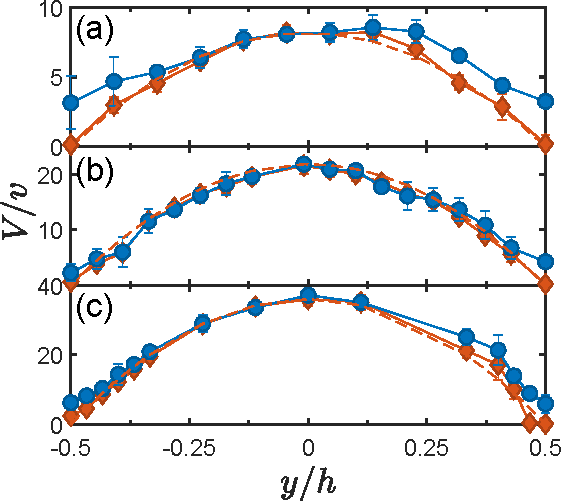
\includegraphics[width=4 in]{Figs/3-Rheo/3.pdf}
	\end{center}
	\caption[Velocity profiles of fluid flows and bacteria at different channel heights]
	{
	\textbf{Velocity profiles of fluid flows and bacteria at different channel heights.}
  The blue disks are the velocity profiles of fluid flows measured frompassive colloidal tracers. The orange diamonds are the velocity profiles of bacteria measured from bacteria.
  (a) $h = 30$ $\mu$m and $\dot\gamma = 25$ s$^{-1}$,
  (b) $h = 50$ $\mu$m and $\dot\gamma = 36$ s$^{-1}$,
  (c) $h = 83$ $\mu$m and $\dot\gamma = 38$ s$^{-1}$.
  The dashed lines are the fittings of parabolic profiles. Velocity is normalized by bacterial velocity $v = 22$ $\mu$m/s.
	}
	\label{fig:3-velocity-profile}
\end{figure}

\subsubsection{Velocity profiles}
First, we measure the velocity profiles of bacterial suspensions along $y$ in microfluidic channels of different heights at low shear rates (Fig.\ref{fig:3-velocity-profile}), where the confinement effect is most pronounced. Near the center of the channels, the velocity profiles of fluid flows, $V(y)$, are parabolic, consistent with the Hagen-Poiseuille law. However, near the bottom and top walls, the velocity of fluid flows measured from passive colloidal tracers noticeably deviates from the parabolic profile and is significantly higher than the velocity of bacteria, $V_{bac}(y)$. Thus, there exists a boundary layer near the confining walls, where bacteria swim against the background flow and exhibit strong relative motions. The thickness of these boundary layers, where strong relative motions of bacteria can be observed, is about 5 $\mu$m, independent of $h$. Thus, as $h$ decreases, the boundary layer plays a more important role in suspension flows. Interestingly, the velocity profiles of bacteria, $V_{bac}(y)$, remain parabolic for different $h$, satisfying the no-slip condition at the walls. Such a feature is
crucial for \textit{E. coli} in natural environments, where they need to maintain their locations in the lower intestine of their hosts against expelling flows.

\begin{figure}[!ht]
	\begin{center}
	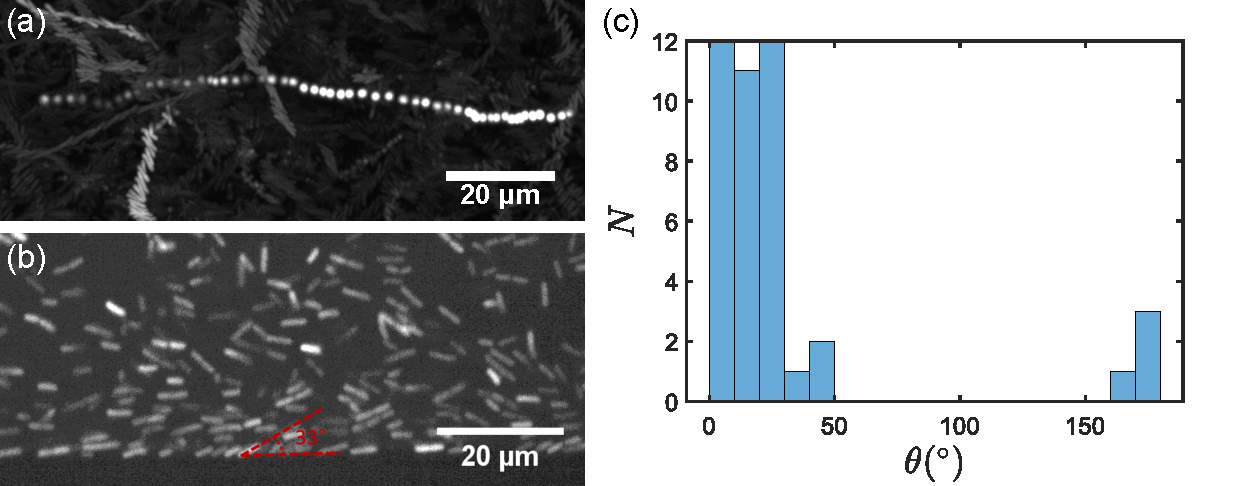
\includegraphics[width=5.5 in]{Figs/3-Rheo/4.pdf}
	\end{center}
	\caption[Upstream swimming bacteria in a microfludic viscometer]
	{
	\textbf{Upstream swimming bacteria.}
   (a) Trajectories of a passive colloidal tracer and bacteria. The maximal intensity of 54 frames over a time interval of 17.5 s is projected onto a single image to show the trajectories. While the spherical passive tracer is transported by the fluid flow, many bacteria swim against the flow and exhibit only transverse motions. The channel height $h = 30$ $\mu$m. The shear rate $\dot\gamma = 24$ s$^{-1}$.
   (b) Bacteria near the side wall, locating at the bottom of the image. The channel height $h = 50$ $\mu$m. The shear rate $\dot\gamma = 7.8$ s$^{-1}$. The direction of the flow is indicated in the images. The orientation of a single bacterium at $\theta = 33$° is indicated.
   (c) Distribution of the orientation of bacteria next to the side wall. The total number of bacteria counted is 42.
	}
	\label{fig:3-upstream}
\end{figure}

\subsubsection{Upstream swimming bacteria}
The difference in the velocity profiles of fluid flows and bacteria indicates the existence of boundary layers near the confining walls consisting of upstream swimming bacteria against imposed shear flows, an observation in agreement with previous experiments \cite{Hill2007, Kaya2012} and simulations \cite{Costanzo2012, Chilukuri2014, Ezhilan2015, Nash2010}. To illustrate the phenomenon directly, Fig.~\ref{fig:3-upstream}a shows the trajectories of colloidal and bacterial tracers near the bottom wall. The relative motions between bacteria and the background fluid can be
clearly identified. The orientation of bacteria against the bottom and top walls can be estimated from the images showing the bacteria near the side walls (Fig.~\ref{fig:3-upstream}b). We plot the distribution of the orientation angle of bacteria against the side walls (Fig.~\ref{fig:3-upstream}c), which strongly biases toward acute angles with the mean at 20°.

\begin{figure}[!ht]
	\begin{center}
	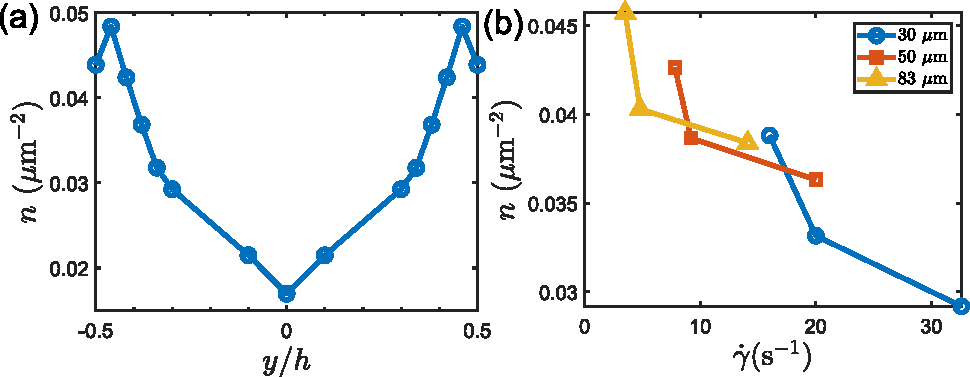
\includegraphics[width=5.5 in]{Figs/3-Rheo/5.pdf}
	\end{center}
	\caption[Bacterial density distribution in microfluidic channels]
	{
	\textbf{Bacterial density distribution in microfluidic channels.}
   (a) Bacterial density across a channel of height $h = 50$ $\mu$m. The shear rate is $\dot\gamma = 7.8$ s$^{-1}$. (b) Bacterial density at the bottom wall as a function of $\dot\gamma$. Different symbols are from channels of different heights, $h$, which are indicated in the figure.
	}
	\label{fig:3-density}
\end{figure}

\subsubsection{Bacterial density distributions}
Finally, we also measure the number density of bacteria in microfluidic channels. Fig.~\ref{fig:3-density}a shows the density distribution of bacterial suspensions along y at a low shear rate. In consistency with previous experiments \cite{Hill2007, Berke2008, Li2009}, we find that bacteria accumulate near the confining walls, an effect arising from the coupling between self-propulsion and steric interactions \cite{Ezhilan2015}. Hydrodynamic interactions between bacteria and solid surfaces also enhance the accumulation \cite{Berke2008}. Furthermore, Fig.~\ref{fig:3-density}b shows bacterial concentrations at the bottom confining wall as a function of shear rates. The concentration decreases with increasing shear rates, leading to more uniform density profiles at high shear rates \cite{Ezhilan2015}.


\section{Discussion and Conclusion}
\subsection{Data analysis}
We performa simple data analysis to better illustrate the origin of the unusual rheology of bacterial suspensions under confinement.
First, we shall recapitulate the calculation for the viscosity ratio of the two miscible fluids in a bulk Y-shaped microfluidic channel. Within the Hele-Shaw approximation, the average velocities of fluid 1 and fluid 2 over the channel height $y$ are given by \cite{Lamb1932}
\begin{equation}
  \langle V_j \rangle = -\frac{1}{12}\frac{h^2}{\eta_j}\frac{\partial P}{\partial x}
\end{equation}
where $\partial P/\partial x$ is the pressure gradient driving the flow, which is the same in the two branches. $j$ can be either 1 or 2, denoting different fluids 1 and 2. $\eta_1$ and $\eta_2$ are the viscosity of fluid 1 and fluid 2, respectively. Thus,
\begin{equation}
  \label{eq:3-2}
  \langle V_1 \rangle \eta_1 = \langle V_2 \rangle \eta_2
\end{equation}
In addition, the flow rates of the two fluids are the same,
\begin{equation}
  \label{eq:3-3}
  \langle V_1 \rangle d_1 h = \langle V_2 \rangle d_2 h
\end{equation}
Combining Eqs.~\ref{eq:3-2} and \ref{eq:3-3}, we obtain the desired relation for the viscometer
$$
	\frac{d_1}{d_2} = \frac{\eta_1}{\eta_2}
$$
In our experiments, fluid 1 is a bacterial suspension with an unknown viscosity of $\eta$. As the reference fluid, fluid 2 is the suspending fluid with a known viscosity $\eta_0$. The relative viscosity of the bacterial suspension is thus \cite{Gachelin2013}
\begin{equation}
  \label{eq:3-4}
  \frac{\eta}{\eta_0} = \frac{d_1}{d_2}
\end{equation}
where $d_1$ is the width of the bacterial suspension and $d_2$ is the width of the suspending fluid. For a confined bacterial suspension, there should be an extra contribution to the fluid flow arising from the coupling between bacterial motility and the confining surfaces of the channel. We assume this extra disturbance flow linearly superposes to the pressure-driven Poiseuille flow at low Reynolds numbers:
\begin{equation}
  \label{eq:3-5}
  \langle V \rangle = -\frac{1}{12}\frac{h^2}{\eta_b}\frac{\partial P}{\partial x} + \langle V_d \rangle
\end{equation}
Here, $\langle V_d \rangle$ is the average strength of the boundary-driven disturbance flow. $\eta_b$ is the viscosity of bulk bacterial suspensions without the influence of system boundary. Numerically, we obtain $\eta_b$ by fitting our experiments on bulk samples with $h > 60$ $\mu$m using an exponential function, which gives $\eta_b/\eta_0=1.3-\exp(-0.24\dot\gamma)$ (Fig.~\ref{fig:3-rheology}a). In bulk samples, the disturbance flow from the boundary is negligible with $\langle V_d \rangle \approx 0$.
The non-trivial rheology results from the active hydrodynamic stresslets and diffusive stresses \cite{Alonso-Matilla2016, Takatori2017}. We shall focus on the confined systems in our analysis below, where boundary-driven disturbance flows dominate. Note that since the characteristic shear rate at which shear thickening occurs in bulk samples is $1/0.24 \approx 4$ s$^{-1}$ smaller than the lowest shear rate we can achieve in confined channels when $h < 60$ $\mu$m (Fig.~\ref{fig:3-rheology}a), the shear thickening effect of bulk samples should not strongly affect our analysis of $\langle V_d \rangle$ below.
Quantitatively similar results on $\langle V_d \rangle$ are indeed obtained if we fix $\eta_b/\eta_0 = 1.3$ in Eq.~\ref{eq:3-5}, i.e.,
the high-shear-rate plateau of the relative viscosity. With the assumption of Eq.~\ref{eq:3-5} as well as the average velocity
of the suspending fluid, which is Newtonian following
\begin{equation}
  \label{eq:3-6}
  \langle V_0 \rangle = -\frac{1}{12}\frac{h^2}{\eta_0}\frac{\partial P}{\partial x}
\end{equation}
we have
\begin{equation}
  \label{eq:3-7}
  \langle V \rangle = \frac{\eta_0}{\eta_b} \langle V_0 \rangle + \langle V_d \rangle
\end{equation}
Furthermore, the flow rates in the two fluids should be the same as before,
$$
  \langle V \rangle d_1 h = \langle V_0 \rangle d_2 h
$$
which leads to
$$
\langle V \rangle = \frac{\eta_0d_1}{\eta_bd_2} \langle V_0 \rangle + \langle V_d \rangle
$$
Experimentally, the relative viscosity, $\eta/\eta_0$, ismeasured via the width ratio of the two fluids. Hence, by definition,
\begin{equation}
  \label{eq:3-8}
  \frac{\eta}{\eta_0} \equiv \frac{d_1}{d_2} = \frac{\eta_b}{\eta_0} \left[ 1 - \frac{\langle V_d \rangle}{\langle V \rangle}  \right]
\end{equation}
Finally, applying the definition of the characteristic shear rate,
$$
\dot\gamma \equiv \frac{6Q}{d_1h^2} = \frac{6\langle V \rangle}{h}
$$
we have
\begin{equation}
  \label{eq:3-9}
  \frac{\eta}{\eta_0} = \frac{\eta_b}{\eta_0} \left[ 1 - \frac{6\langle V_d \rangle}{h\dot\gamma}  \right]
\end{equation}


\begin{figure}[!ht]
	\begin{center}
	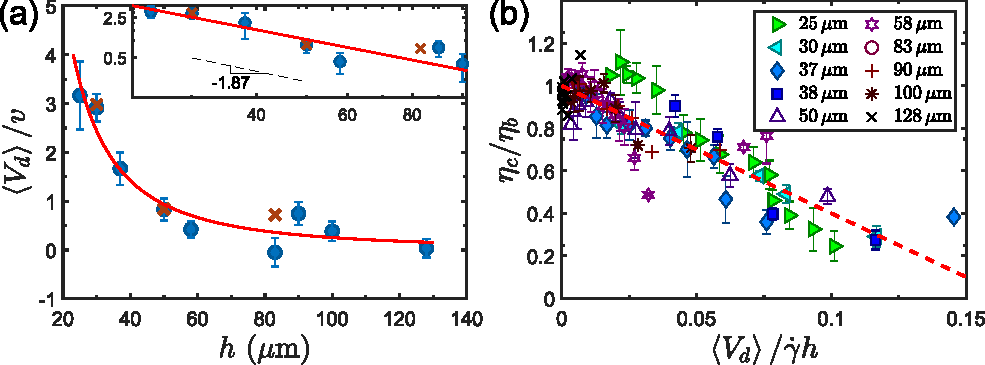
\includegraphics[width=5.5 in]{Figs/3-Rheo/6.pdf}
	\end{center}
	\caption[Scaling of relative viscosity of bacterial suspensions]
	{
	\textbf{Scaling of relative viscosity.}
   (a) The average velocity of the boundary-driven disturbance flows, $\langle V_d \rangle$, as a function of the channel height, $h$. Blue disks are from the fitting of Eq.~\ref{eq:3-9}. Red crosses are from the direct velocity-profile measurements (Fig.~\ref{fig:3-velocity-profile}). $\langle V_d \rangle$ is normalized by the swimming speed of bacteria $v = 22$ $\mu$m/s. The solid red line is a power-law fitting, $\langle V_d \rangle \sim h^{-1.87}$. Inset shows the same data in a log-log plot.
   (b) Viscosity ratio, $\eta/\eta_b$, as a function of inverse dimensionless shear rates, $\langle V_d \rangle / h\dot\gamma$. $h$ is indicated in the plot. The dashed line indicates $y = 1 – 6x$, the prediction of Eq.~\ref{eq:3-9}.
  }
	\label{fig:3-scaling}
\end{figure}


We fit our experimental results using the above equation, where $\eta_b/\eta_0$ is given by the exponential function for bulk samples as discussed above. $\langle V_d \rangle$ is taken as a fitting parameter, which we assume is independent of $\dot\gamma$. We find that $\langle V_d \rangle$ decreases with increasing $h$ and shows an approximate power law scaling, $\langle V_d \rangle \sim h^{-\alpha}$, with $\alpha = - 1.9 \pm 0.6$ (Fig.~\ref{fig:3-scaling}a).
$\langle V_d \rangle$ obtained from the fitting quantitatively agrees with direct measurements based on the velocity profiles (Fig.~\ref{fig:3-velocity-profile}), where the disturbance flow can be extracted by subtracting the parabolic bacterial flow from the total fluid flow, $V_d(y) = V(y) - V_{bac}(y)$. Using $\langle V_d \rangle$, a good collapse of data can be achieved by plotting the viscosity ratio $\eta/\eta_b$ versus the inverse dimensionless shear rate $\langle V_d \rangle / h\dot\gamma$ (Fig.~\ref{fig:3-scaling}b).
A linear trend predicted by Eq.~\ref{eq:3-9} can be clearly identified. We shall discuss the possible origin of $\langle V_d \rangle$ below.

\subsection{Effect of active hydrodynamic and diffusive stresses}

Using a kinetic theory with active hydrodynamic stresslets, Alonso-Matilla and co-workers studied the effect of confinement
on the rheology of bacterial suspensions \cite{Alonso-Matilla2016}. Since bacterial density is higher near the confining walls (Fig.~\ref{fig:3-density}a), as the system size reduces, the regions with higher bacterial density near the walls start to overlap near the center of microfluidic channels. As a result, relatively fewer bacteria are subject to the high shear near the walls, mitigating the effect of shear alignment and viscosity reduction. Hence, the viscosity of confined bacterial suspensions was predicted
to be higher than that of bulk suspensions at the same shear rate, which is opposite to our experimental observations.

The effect of diffusive stresses in confined systems is more complicated. The hydrodynamic stress from active stresslet scales as $\sigma^H \sim n\zeta v a$, which therefore does not directly depend on the confinement except via bacterial density $n$ as discussed
above. Here, $\zeta$ is the drag coefficient and a is the characteristic size of the bacteria. In comparison, the diffusive stress scales as $\sigma^S \sim n \zeta v L$, where $L$ is the run length of bacteria \cite{Takatori}. In confined systems, bacterial run length is determined by the size of a system. In a simple picture, $L$ should be replaced by the size of system h as $\sigma^S \sim n \zeta v h$, which gives rise to a direct system-size dependence. The magnitude of $\sigma^S$ decreases with increasing confinement. Whether the viscosity of bacterial suspensions increases or decreases with $h$ depends on the sign of $\sigma^S$. In the low Peclet number (Pe) limit where the diffusive stress dominates, $\sigma^S$ is negative. As a result, when h decreases, the magnitude of $\sigma^S$ decreases and the viscosity of suspensions increases with the decreasing $h$, opposite to our experiments.
However, for intermediate Pe that is more relevant to our experiments, $\sigma^S$ becomes positive (see Fig. 2 of Ref.~\cite{Takatori2017}), which leads to the reduction of viscosity in confined systems, consistent with our experiments. Nevertheless, for suspensions of spherical particles, where the analytical solution of the viscosity is available (Eq. 5 of Ref.~\cite{Takatori2017}), the decrease of viscosity is less than a factor of 1.1 when we decrease $h$ from 50 to 25 $\mu$m even at the optimal shear rates of 2.1 s$^{-1}$ that leads to the largest viscosity reduction. In comparison, the viscosity decreases by more than a factor of 3 over the same range of $h$ in our experiments. Although the analytical solution for suspensions of active ellipsoids appropriate for the bacteria is not available, numerical solutions show that the magnitude of $\sigma^S$ of active ellipsoids is smaller than that of active spheres \cite{Takatori2017}. Hence, we expect that the effect of the confinement-induced viscosity reduction is even weaker for suspensions of active ellipsoids.
This conclusion is supported by the failure of our attempt to collapse data using a dimensionless shear rate with the characteristic run-time of bacteria (Fig.~\ref{fig:3-rheology}b). Thus, other factor(s) need to be considered to fully explain the experimental observations.

\begin{figure}[!ht]
	\begin{center}
	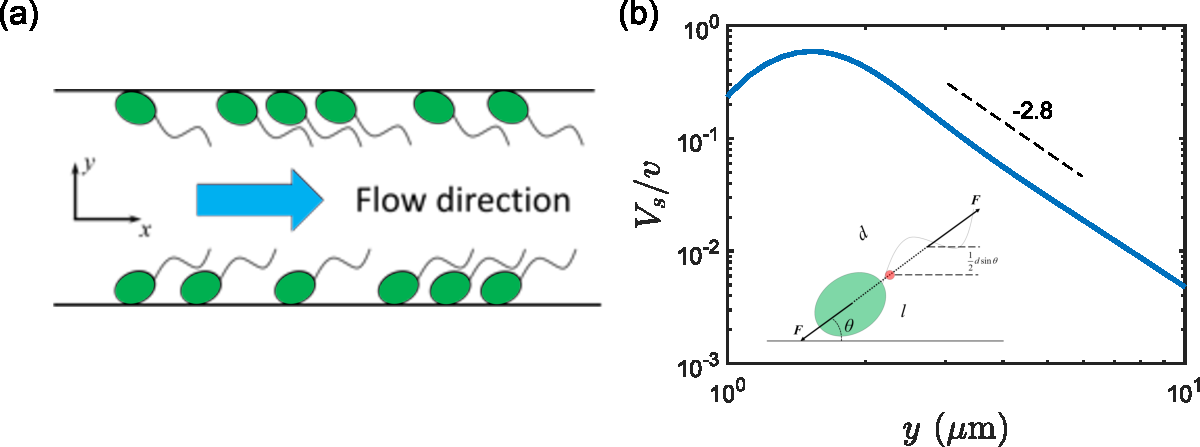
\includegraphics[width=5.5 in]{Figs/3-Rheo/7a.pdf}
	\end{center}
	\caption[Boundary-layer upstream swimming bacteria model]
	{
	\textbf{Boundary-layer upstream swimming bacteria model.}
  (a) Schematic of boundary-layer upstream swimming bacteria model.
  (b) Velocity induced by a single dipole, Vs, as a function of the distance to a flat wall, l. The dashed line indicates a power-law scaling $V_s \sim l^{-2.8}$. The inset shows the force dipole of a single bacterium next to the wall with all relevant parameters defined in the main text. The pink disk indicates the center of the force dipole, whereas the blue disks indicate the locations of the upper and lower Stokeslets.
  }
  \label{fig:3-model}
\end{figure}


\subsection{Effect of upstream swimming bacteria at boundary}

A possible origin of $\langle V_d \rangle$ is the boundary layer of upstream swimming bacteria. To estimate their effect, we numerically calculate $\langle V_d \rangle$ by assuming a smectic layer of upstream swimming bacteria in a 2D channel with a line density $n$ randomly distributed along the top and bottom walls (Fig.~\ref{fig:3-model}a). Since a bacterium is force-free at low Reynolds numbers, the far-field disturbance flow induced by the bacterium is a hydrodynamic dipolar flow.
The flow of a single force dipole near the walls can be constructed by superposition of two Stokeslets of strength $F$ at position $\mathbf{r_0} + \mathbf{u}d/2$ and $\mathbf{r_0} - \mathbf{u}d/2$, respectively, where $\mathbf{r_0} = (x_0, y_0)$ is the center of the force dipole (Fig.~\ref{fig:3-model}b inset). We fix $y_0$ at 1 $\mu$m away from the walls in our calculation.
The classical solution of a Stokeslet near a wall is used in this construction \cite{Blake1971}, so that the disturbance flow satisfies both the no-penetration and the no-slip boundary conditions at the closest wall. d = 2.2 $\mu$m is the distance between
the two Stokeslets in a force dipole obtained from experiments \cite{Drescher2011}. $\mathbf{u}$ indicates the direction of the force
dipole, which forms an acute angle $\theta$ against the imposed shear flow. We choose $\theta = 20$°, the mean angle of bacterial
orientation from our experimental observations. Other acute angles lead to qualitatively similar results. $F$ is related to bacterial
swimming speed $v$ through $F = \zeta v$ with $F \approx 0.43$ pN for \textit{E. coli} \cite{Drescher2011}. The disturbance flow is translationally invariant along $x$ for infinite large systems. In our calculation, we set the system size to be 1 mm in $x$, much larger than the average spacing between dipoles. The disturbance flow is then obtained near the center of the system. Specifically, we compute the x-component disturbance flow, $V_d(y)$, at a fixed $x$ defined as $x = 0$. All the results are averaged over 100 different random configurations. To avoid the singularity at $x = 0$, we exclude those configurations where the locations of the Stokeslets fall in $x \in$ [-10 nm, 10 nm].
A cutoff, $l_c$, in $y$ can be further chosen based on $\int_{-h/2}^{-h/2+l_c} V_d(y)dy = 0$, below which the near-field bacterial flow is important and the dipole-flow approximation of our simple model breaks down.
$l_c \sim 1.4$ $\mu$m, slightly higher than the location of the upper Stokeslet.

\begin{figure}[!ht]
	\begin{center}
	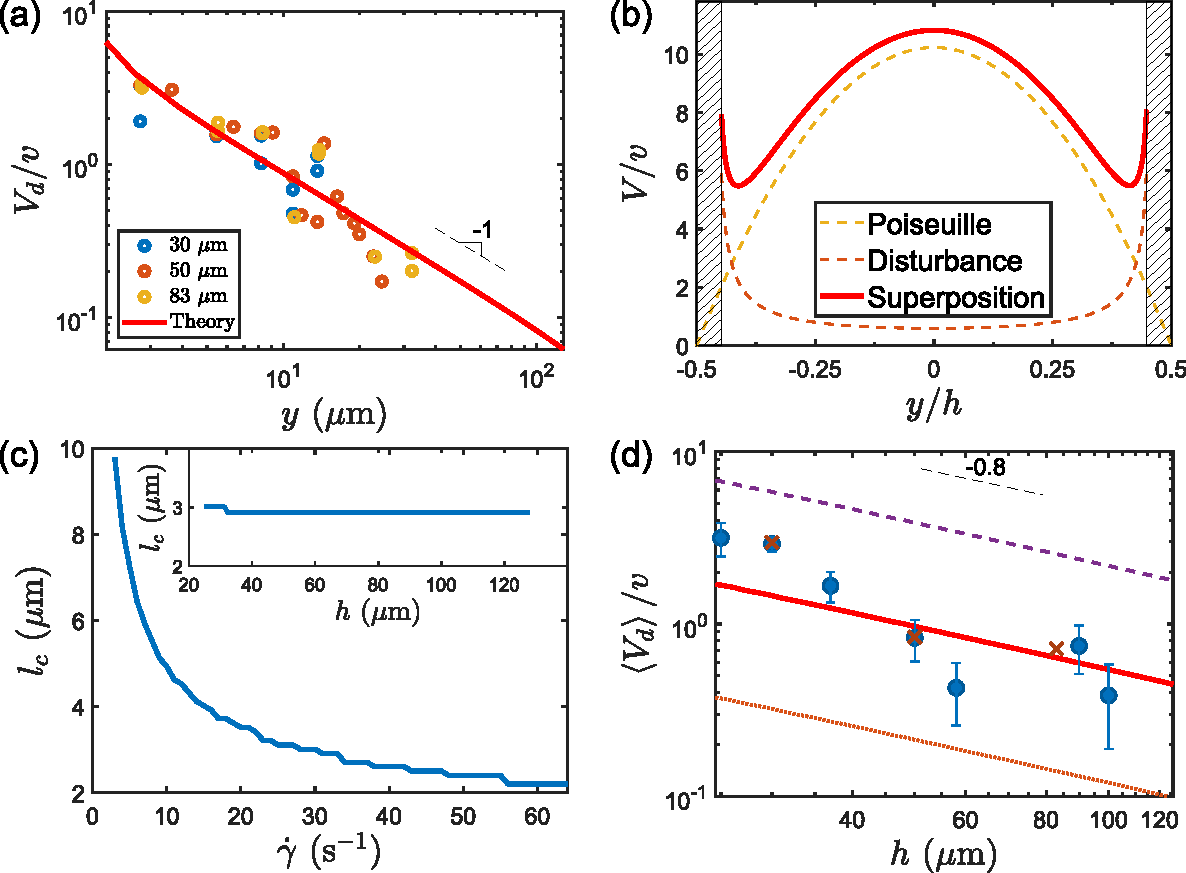
\includegraphics[width=5.5 in]{Figs/3-Rheo/7b.pdf}
	\end{center}
	\caption[Compare boundary-layer model with experimental data]
	{
	\textbf{Compare boundary-layer model with experimental data.}
  (a) Velocity profile induced by a line of randomly distributed dipoles at dipolar line density $n = 2$ $\mu$m$^{-1}$. Symbols are from experiments at different channel heights, which are indicated in the figure. The dashed line indicates a power-law scaling $V_d \sim l^{-1}$.
  (b) Velocity profiles in a channel of height $h = 30$ $\mu$m and shear rate $\dot\gamma=30$ s$^{-1}$. The brown dashed line is the disturbance velocity profile, $V_d(y)$. The yellow dashed line is the parabolic Poiseuille flow. The red solid line is the superposed velocity profile, $V(y)$. The shaded regions are within the cutoff $l_c$.
  (c) Thickness of the boundary layer, $l_b$, versus $\dot\gamma$ with $h = 30$ $\mu$m and $n = 2$ $\mu$m$^{-1}$. Inset: $l_c$ as function of $h$ with $\dot\gamma = 30$ s$^{-1}$.
  (d) The average disturbance flow velocity $\langle V_d \rangle$ as a function of h at different bacterial densities. Symbols are from experiments in Fig. 6a. Bacterial density: $n = 0.2$ $\mu$m$^{-1}$ (brown dotted line), 1.0 $\mu$m$^{-1}$ (red solid line) and 4 $\mu$m$^{-1}$ (purple dashed line). The black dashed line indicates a power-law scaling $\langle V_d \rangle \sim h^{-0.81}$. All the velocities are normalized by the swimming speed of bacteria $v = 22$ $\mu$m/s.
  }
  \label{fig:3-model-compare}
\end{figure}


For a single bacterium near the wall, the disturbance flow decays as $V_s\sim l^{-2.8}$, faster than the decay of a dipolar
flow in bulk, where $l$ is the distance away from the wall (Fig.~\ref{fig:3-model}b).
Collectively, the disturbance flow from the smectic layer of randomly distributed bacteria decays much slower as $V_d \sim l^{-1}$, quantitatively agreeing with our velocity-profile measurements (Fig.~\ref{fig:3-model-compare}a). By comparing the experiments and calculation, we obtain the effective dipole density at the wall $n = 2$ $\mu$m$^{-1}$. Near the center of the channel away from the walls, $V_d$ is small. The fluid is dominated by the pressure-driven Poiseuille flow and is approximately parabolic in shape, consistent with our experiments (Fig.~\ref{fig:3-model-compare}b). We estimate the thickness of the boundary layer, $l_b$, by the location where the superposed velocity profile shows a minimum. Below $l_b$, the disturbance flow from the upstreaming bacteria dominates the
Poiseuille flow. We find that $l_b$ is a weak function of $h$ over the range of $\dot\gamma$ in our experiments (Fig.~\ref{fig:3-model-compare}c inset), confirming that the disturbance flow induced by the upstreaming bacteria is confined within a boundary layer. Moreover, $l_b$ decreases with increasing $\dot\gamma$ (Fig.~\ref{fig:3-model-compare}c).
At high $\dot\gamma$ , the boundary layer becomes insignificant, consistent with our observation (Fig.~\ref{fig:3-rheology}c). At $\dot\gamma = 30$ s$^{-1}$, $l$ is about 3 $\mu$m, qualitatively agreeing with our observations.

Finally, the average strength of the disturbance flow, $\langle V_d \rangle$, is calculated by integrating the disturbance velocity
profile over the channel height. $\langle V_d \rangle$ as a function of $h$ is shown in Fig.~\ref{fig:3-model-compare}d. At a fixed $h$, $\langle V_d \rangle$ increases linearly with bacterial density. More importantly, $\langle V_d \rangle$ decreases with $h$,
agreeing with our experimental observations qualitatively (Fig.~\ref{fig:3-model-compare}d). The best fitting gives $n = 1.0$ $\mu$m$^{-1}$, comparable with the fitting from Vd(l). Numerically, we find $\langle V_d \rangle \sim h^{-0.81}$, with a scaling exponent smaller than that of the experiments. Although the disturbance flow induced by a single bacterium near the wall decays as $l^{-2.8}$, too weak to influence the macroscopic fluid flows driven by pressure gradients, the formation of the boundary layer allows such a weak effect from individual bacteria to add coherently, which strongly modifies the fluid flows of bacterial suspensions in confined channels. Hydrodynamic simulations have further shown that coherent structures of active particles including layers of upstream swimming bacteria emerge in confined geometries when the run length of active particles exceeds the confinement length \cite{Nash2010}. Such a finding provides a possible explanation why the confinement effect is most obvious when the system size is comparable or below the run length of bacteria in our experiments.

Although the velocity profiles and the power-law scaling can be qualitatively explained by the presence of the boundary layers of upstream swimming bacteria, there are still open questions on the hypothesis. First, at the experimental bacterial density of ~ 0.2 $\mu$m$^{-1}$, the strength of the disturbance flow $V_d$ calculated from our simple model is about 5 times weaker than that from our experiments (Fig.~\ref{fig:3-model-compare}d). Such a discrepancy may be accounted for by considering a finite thickness of the boundary layer and including multiple bacterial layers near the confined walls. Second, the calculated velocity profile oscillates strongly within the cutoff length of the boundary layer due to the singular nature of the dipole flow (Fig.~\ref{fig:3-model-compare}b). The dipole flow describes the far-field flow of the bacteria quantitatively but provides only a qualitative trend in the near field \cite{Drescher2011, Mathijssen2016}. Thus, to quantify the disturbance flow within the boundary layer close to the bacteria, detailed  understanding of the near-field bacterial flow is needed. Third, the upstream swimming behavior of bacteria depends on the strength of external flows \cite{Kaya2012}.
Bacterial concentrations next to the walls are also a function of shear rate and system size (Fig.~\ref{fig:3-density}b). These effects will likely lead to the dependence of $V_d$ on $\dot\gamma$ and $h$, which are not included in our qualitative discussion above. The lack of these dependences may explain the smaller scaling exponent of $\langle V_d \rangle(h)$ in our model. Lastly, it is worth noting that both active hydrodynamic and diffusive stresses are still present in confined bacterial suspensions. In the bulk limit, the contribution of the boundary-driven disturbance flow diminishes. Active hydrodynamic stresslets and diffusive stresses
become the leading reason of the non-trivial rheology of active fluids \cite{Alonso-Matilla2016, Takatori2017}. Thus, their contributions should also be included in formulating a quantitative theory of active fluids under confinement. We hope our simple heuristic model on the upstream swimming bacteria, an effect that is missing in previous theories, can stimulate further theoretical development.

In summary, we experimentally studied the rheology of confined bacterial suspensions using a microfluidic viscometer. A confinement
effect was observed at low shear rates, where the viscosity of bacterial suspensions decreases with increasing confinement. We showed that such a confinement effect arises from the interplay between bacterial motility and confining surfaces. A simple analysis was developed to reveal the physical origin of the confinement effect. We proposed that the boundary layers near confining surfaces, where bacteria collectively swim against the imposed shear flows, play a key role in determining the flow structure and the rheology of confined bacterial suspensions. A simple model based on this picture shows a qualitative agreement with our macroscopic rheology
and microscopic dynamics measurements. Open questions were finally discussed for future theoretical development. As such, our experiments demonstrate the importance of system boundary on the flow of bacterial suspensions and present a benchmark to verify different models of the rheology of active fluids. The results are also potentially useful in designing new strategies to modify bacterial transport in confined geometries.


\chapter[Giant Number Fluctuations in 3-Dimensional Space]{Giant Number Fluctuations in 3-Dimensional Space}
\label{giant-number-fluctuations-in-3-dimensional-space}
%%%%%%%%%%%%%%%%%%%%%%%%%%%%%%%%%%%%%%%%%%%%%%%%%%%%%

\section{Introduction}
Active fluids exhibit many unusual behaviors beyond the expectation of equilibrium statistical mechanics \cite{Ramaswamy2010,Cates2012,Marchetti2013,Poon2013,Elgeti2015}.
In particular, an active fluid can exhibit anomalously large density variations, the so-called giant number fluctuations (GNF), where the standard deviation of the number of particles grows nonlinearly with the square root of the mean particle number, defying the central limit theorem of equilibrium systems \cite{Mishin2015}.
Such unusual density fluctuations have been observed in a wide range of active fluids in both living and non-living systems including vibrated granular rods \cite{Narayan2007,Aranson2008,Kudrolli2008,Deseigne2010},
swarming bacteria \cite{Zhang2010,Nishiguchi2017} and mammalian cells \cite{Kawaguchi2017},
self-propelled cytoskeleton \cite{Schaller2013}, and synthetic colloidal swimmers \cite{Palacci2013,Karani2019}. As a result, GNF has generally been viewed as a hallmark of the emergent behaviors of active fluids.


Significant theoretical and computational advancement on GNF has been made over the past two decades since the seminal works of Toner and Tu \cite{Toner1995,Tu1998,Toner1998,Simha2002,Ramaswamy2003,Toner2005,Chate2008,Mishra2010,
Dey2012,Saintillan2012,Saintillan2013,Ngo2014,Mahault2019}. Meanwhile, many important theoretical and numerical predictions have been tested in experimental realizations
\cite{Narayan2007, Aranson2008, Deseigne2010, Zhang2010, Schaller2013,
Nishiguchi2017, Kawaguchi2017, Palacci2013}.

Of particular interest is the scaling exponent $\alpha$, which is defined following $\Delta N /\sqrt N \propto N^\alpha$, where $\Delta N$ is the standard deviation of particle number and $N$ is the mean number of particles in a subsystem of given size. Heretofore, all the existing experiments on GNF were limited to two-dimensional (2D) or quasi-2D systems. In contrast to theoretical predictions (where $\alpha \approx 0.3$), $\alpha$'s obtained in these experiments show large variations ranging from 0.13 to 0.5. Such a large variation arises partially because of complicated particle-boundary interactions, which are hard to incorporate in theoretical studies. Moreover, the predictions of $\alpha$ in three-dimensional (3D) wet active fluids---one of the most important classes of active fluids where hydrodynamics dominate the interparticle interactions and conserve the total momentum of systems \cite{Marchetti2013}---has not been experimentally testified. Therefore, there is an imperative need for an experimental measurement of $\alpha$ in 3D active fluids, which are not affected by system boundaries. Such a measurement will provide not only an unambiguous experimental benchmark to testify theories of active fluids, but also experimental support on the effect of dimensionality on GNF of active fluids \cite{Marchetti2013}.

The rise of GNF in active fluids is usually accompanied by the transition to ordered phases with collective motions \cite{Ramaswamy2010,Marchetti2013}. For wet 3D active fluids such as bacterial suspensions, these collective motions lead to large-scale coherent flows with intermittent vortices and jets, which are often referred to as active turbulence \cite{Wolgemuth2008,Wensink2012,Dunkel2013a,Bratanov2015,Guo2018,Linkmann2019,Bardfalvy2019,Alert2020,Skultety2020,Peng2020}. Similar to GNF that manifests density fluctuations across different scales, the flow of active turbulence also exhibits scale-dependent structures.
Imported from the study of classical turbulence, energy spectra are frequently measured to quantify such structures in active turbulence \cite{Ishikawa2011,Wensink2012,Dunkel2013a,Giomi2015,Creppy2015,Patteson2018,Alert2020}. Although both GNF and energy spectra quantify the scale-dependent dynamics of active fluids, the deep connection between these two quantities at different scales has not been experimentally investigated. Our experiment reveals the density- and scale- independent coupling between GNF and energy spectra, suggesting that GNF is governed by the strength of the motion-induced flow.

\begin{figure}[htbp]
\begin{center}
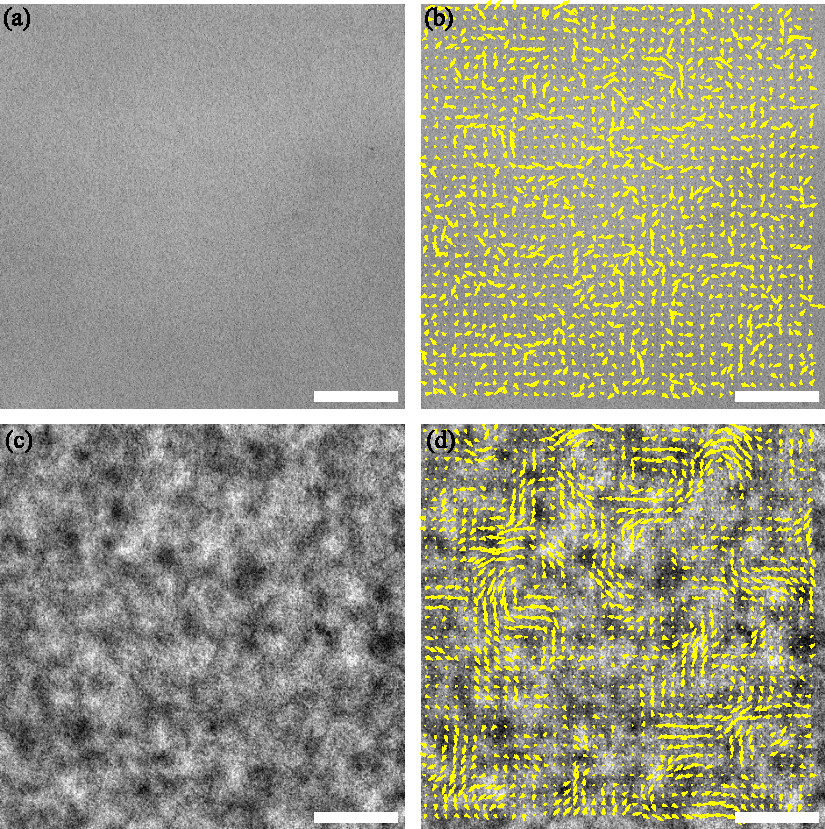
\includegraphics[width=5.5in]{figs/5-GNF/1.pdf}
\caption[Images of Bacterial Active Turbulence and Its Flow Fields]
{
\textbf{Images of bacterial active turbulence and its flow fields.}
(a) and (b) are active turbulence in a dense bacterial suspension (1.6\%) displaying constantly varying concentration inhomogeneity and the corresponding flow field.
(c) and (d) are a dilute bacterial suspension (6.4\%) and the corresponding flow field.
Scale bars are 85 $\mu$ m.
}
\label{fig:experiment}
\end{center}
\end{figure}


\section{Methods}

\subsection{Sample Preparation, Imaging and Analysis}
Here, we present our systematic experimental study of GNF and energy spectra in bulk bacterial suspensions, a premier example of 3D wet active fluids. We use genetically engineered light-powered \textit{Escherichia coli} (\textit{E. coli}) as our model bacteria.
For a typical experiment, a bacterial suspension of control volume fraction $\phi$ is injected into a sealed chamber of 20 mm $\times$ 3 mm $\times$ 140 $\mu$m.
Without supply of oxygen, bacteria quickly consume all the remaining oxygen in the chamber and stop moving after $5$ minutes.
We then illuminate the suspension with a high-intensity microscope light, which powers bacteria at their maximal swimming speed of $15 \pm 3$ $\mu$m/s in the dilute limit.
A video of the suspension is taken 50 $\mu$m above the bottom wall of the chamber by a bright-field inverted microscope at a frame rate of $30$ fps and the field of view of $420 \times 360$ $\mu$m$^2$ (Fig.~\ref{fig:experiment}a, c).
We use a standard Particle Image Velocimetry (PIV) algorithm \cite{OpenPIV-website}
to extract the 2D in-plane velocity field $(v_x,v_y)$ in the 3D suspension, which exhibits the characteristic chaotically-moving vortices and jets of active turbulence at high $\phi$ (Fig.~\ref{fig:experiment}b, d).

\subsection{The Relation between Pixel Intensity and Concentration}

It is challenging to directly count the number of bacteria in a 3D suspension of fasting moving bacteria. Luckily, by virtue of Beer-Lambert law, the local bacterial density is monotonically correlated with the local intensity of microscope images, where darker regions correspond to higher bacterial densities (Fig.~\ref{fig:experiment}c). Similarly principles also appeared in other experimental works, where optical information was exploited in probing the dynamics in suspensions of bacteria and actin filaments \cite{Sokolov2009, Wilson2011, Schaller2013}.

\begin{figure}[ht]
\begin{center}
\includegraphics[width=3.5in]{figs/5-GNF/2.pdf}
\caption[Relation between Image Intensity and Concentration]
{
\textbf{Relation between image intensity and concentration.}
(a) Images of bacterial suspensions of different volume fractions under the same illumination conditions.
(b) Volume fractions as a function of average pixel intensities.
}
\label{fig:calibration}
\end{center}
\end{figure}

To calibrate the density-intensity correlation, we prepare bacterial suspensions of different $\phi$ and image the suspensions under the same illumination (Fig.~\ref{fig:calibration}a). The mean image intensity decreases with increasing $\phi$ following an approximately linear relation (Fig.~\ref{fig:calibration}b), agreeing with the the Beer-Lambert law for samples of small thickness and weak absorptivity appropriate for our experiments. The linear density-intensity relation has also been used in previous experiments on \textit{E. coli} suspensions \cite{Wilson2011}.

In the low attenuation limit (small thickness and weak absorptivity), $I=I_0-\epsilon$ where $\epsilon\ll I_0$:
\begin{equation}
  \log \frac{I_0}{I} = \log \frac{I_0}{I_0 - \epsilon} \approx \frac{\epsilon}{I_0} \sim c
\end{equation}
\begin{equation}
I = I_0 - \epsilon \sim c
\end{equation}
where $I_0$ is the original light intensity, $I$ is the transmission light intensity, $\epsilon$ is the attenuated light intensity, which is much smaller than the original light intensity.

\begin{figure}[ht]
\begin{center}
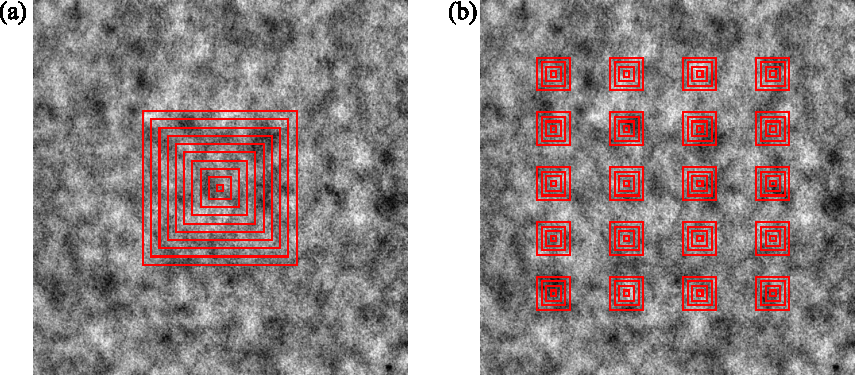
\includegraphics[width=0.9\textwidth]{figs/5-GNF/GNF-calculations.pdf}
\caption[GNF Calculations]
{
\textbf{GNF calculations.}
(a) Varying subsystem sizes.
(b) Multiple seeds of subsystems for spatial average.
}
\label{GNF-calculation}
\end{center}
\end{figure}

\subsection{GNF Calculations}
In Fig.~\ref{fig:calibration}b, we show that under the same illumination and imaging condition, bacterial density and the average pixel intensity follow approximately a linear relation, which can be expressed as follows:
\begin{equation}
\label{eq:phi-I-relation}
\phi = a + bI,
\end{equation}
where $\phi$ is the volume fraction of bacterial suspensions, $I$ is the average pixel intensity, $a$ and $b$ are constants at the fixed illumination and imaging condition. The number of bacteria in a given subsystem of side length $l$ and thickness $d$ can be calculated as
\begin{equation}
\label{eq:n}
N = \frac{l^2d}{V_b} \phi = \frac{l^2d}{V_b} (a+bI),
\end{equation}
where $V_b$ is the volume of a single bacterium. $d \approx 6$ $\mu$m is the depth of the field of microscopy, which is fixed in our experiments. Thus, the number of bacteria in the subsystem $N$ is proportional to $l^2 \phi$. Taking the standard deviation of both sides of Eq.~\ref{eq:n}, we obtain
\begin{equation}
\label{intensity-number}
\Delta N = \frac{l^2 d}{V_b}|b|\Delta I,
\end{equation}
where $\Delta N$ is the standard deviation of the bacterial number in the subsystem over time and $\Delta I$ is the standard deviation of the average pixel intensity of the subsystem over time. Since $d|b|/V_b$ is a constant independent of subsystem sizes and bacterial volume fractions, $\Delta N$ is linearly proportional to $l^2\Delta I$. Because any constant in front of $\Delta N$ would not affect either the scaling relation or the relative magnitude of density fluctuations at different $\phi$, we simply take $l^2\Delta I$ as $\Delta N$ in our study.

Based on the linear relation between $\Delta N$ and $\Delta I$, we calculate the density fluctuations at different length scales. We first crop square-shape subsystems of increasing sizes, as shown in Fig.~\ref{GNF-calculation}. For each subsystem size $l$, the standard deviation of the average pixel intensity of the subsystem is calculated over 50 frames (1.67 s or 8.35$\tau_b$), which is longer than the saturated density correlation time of $4\tau_b = 0.8$ s (Fig.~\ref{fig:spatiotemporal-correlations}f). To improve statistics, we choose 20 subsystems of the same size evenly distributed in the field of view and obtain a spatial average of the temporal standard deviation of the average pixel intensity $\Delta I$ (Fig.~\ref{GNF-calculation}). This averaged $\Delta I$ is then multiplied by $l^2$ to give the number density fluctuations $\Delta N$ at the length scale $l$. Note that a second method has also been proposed for calculating number fluctuations, where the standard deviation of particle numbers is computed first spatially over different locations in a single time frame and is then averaged over time of different frames \cite{Aranson2008}.  Although the two methods lead to the same results when spatial and temporal correlations are small compared with the system size and experiment duration \cite{Aranson2008}, the second method is subject to potential systematic errors in our study due to time-independent non-uniform light illumination and intrinsic stationary density variations in non-motile suspensions at $t=0$ in the kinetic measurements. Using the first method, any stable non-uniform light illumination or stationary non-uniform density variations would result in zero temporal standard deviations of $I$ and, therefore, would not affect our measurements of true density fluctuations of motile bacterial suspensions.


\subsection{Normalization of GNF at Different Volume Fractions}

Practically, to optimize image qualities, we adjust the exposure time of imaging for suspensions of different $\phi$. Exposure times affect the proportional constant $b$ in Eq.~\ref{eq:phi-I-relation}, which introduces a $\phi$-dependent linear constant $b(\phi)$ in Eq.~\ref{eq:n}. Although $b(\phi)$ does not affect the scaling exponent of density fluctuations $\alpha$, it modifies the relative magnitude of $\Delta N$ at different $\phi$. In order to compare the magnitude of density fluctuations at different $\phi$,  we further calibrate and normalize $\Delta I$ for different $\phi$. Specifically, as the calibration, we take videos of bacterial suspensions at different $\phi$ under the exact same imaging condition with fixed illumination light intensity, condenser position, optical filters and all the camera settings such as the exposure time and the dynamic range. The calibration results are shown in Fig.~\ref{fig:same-conditions}, where $\Delta N \sim l^2 \Delta I$ at different $\phi$ collapse at small length scales. The calibration results show that we can normalize $l^2 \Delta I$ of different exposure times by its value at a fixed small length scale. We choose the small scale at $l = 0.3l_b$ in our study. Since $l^2 \Delta I$ at different $\phi$ shows the same slope at small $l$, choosing any other small lengths between $0.1l_b$ and $0.5l_b$ would lead to quantitatively the same results. The normalized density fluctuations show not only the correct scaling exponents but also the right relative magnitudes at different $\phi$.

\begin{figure}[ht]
  \begin{center}
    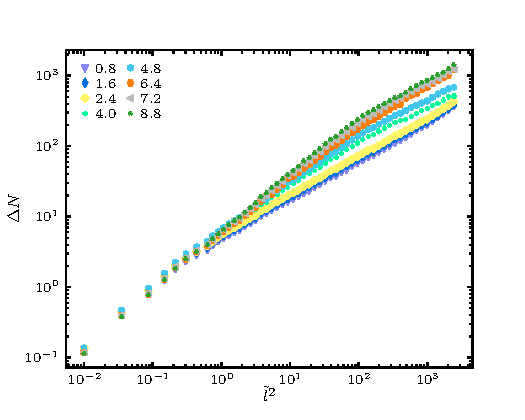
\includegraphics[width=4.5in]{Figs/5-GNF/GNF-normalization.pdf}
    \caption[Normalization of GNF at Different Volume Fractions]
    {
    Calibration of the standard deviation of bacterial number $\Delta N \sim l^2\Delta I$ at different volume fractions $\phi$. $\Delta N$ versus the dimensionless subsystem size $\tilde{l}^2 = l^2/l_b^2$ for bacterial suspensions at different $\phi$. The images are taking under the same illumination with the same imaging condition.
    }
    \label{fig:same-conditions}
  \end{center}
\end{figure}

\subsection{Correlation of Local Density Fluctuations and Kinetic Energies}

To calculate local temporal density fluctuations, we need to approximate instantaneous intensity variations. On the one hand, the time interval for calculating the intensity difference between two frames needs to be smaller than the density correlation time ($4\tau_b = 0.8$ s) in order to satisfy the instantaneous approximation. On the other hand, the time interval should be sufficiently long to suppress the influence of random fluctuations of image intensities in adjacent frames. In our study, we choose 0.3 s (10 frames) for the local density fluctuation calculation. We do not expect the results to be much different when varying this number from 0.17 to 0.6 s.

To calculate the local density variations at the length scale of $l = 2.75l_b$ and time $t$, we take 10 consecutive frames following the frame at $t$. All the 10 frames are first coarse-grained by averaging the intensity of pixels in square windows of size $2.75l_b \times 2.75l_b$ into single coarse-grained pixels (Fig.~\ref{fig:coupling-calculation}b). We then take the temporal standard deviation of the coarse-grained pixel intensity over the 10 frames at different positions to obtain a field of density fluctuations at $t$, $\delta N(\bm{r},t)$, as shown in Fig.~\ref{fig:coupling-calculation}d. The same approach has also been used to calculate the field of instantaneous density fluctuations in the transient state shown in Fig.~\ref{fig:GNF-energy-spectra-correlation-transient}a.

Independently, the PIV algorithm is also applied on the original images of the first two frames to obtain the velocity field at time $t$, $\bm{v}(\bm{r},t)$ (Fig.~\ref{fig:coupling-calculation}c). Since the step size of the PIV analysis is also at $2.75l_b$, the velocity field has the same dimensions as the coarse-grained density fluctuation field obtained above. The local kinetic energy can then be calculated as $E(\bm{r},t)=|\bm{v}(\bm{r},t)|^2/2$ (Fig.~\ref{fig:coupling-calculation}e). Finally, the normalized correlation between $\delta N(\bm{r},t)$ and $E(\bm{r},t)$ is computed as
\begin{equation}
C_s = \frac{\langle(\Delta N-\overline{\Delta N})(E-\overline{E})\rangle}{\sigma_{\Delta N}\sigma_{E}},
\end{equation}
where $\bar A$ indicates the mean of variable $A$, $\sigma_A$ indicates the standard deviation of $A$, and $\langle A \rangle$ denotes the average of $A$ over all the positions. The correlation quantifies the spatial similarity between $\delta N$ and $E$, which ranges between $-1$ to 1. Finally, the correlation $C$ shown in Fig.~\ref{fig:GNF-energy-spectra-correlation}b is calculated by averaging $C_s$ over 1000 frames.

\begin{figure}[!]
	\begin{center}
		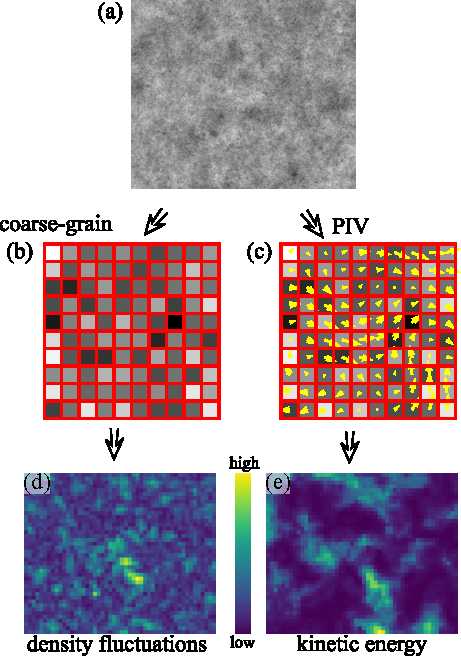
\includegraphics[width=3.5in]{Figs/5-GNF/local-correlation.pdf}
		\caption[Local Correlation between Density Fluctuations and Kinetic Energies]
		{
			Diagram showing the procedure to calculate the correlation between local density fluctuations and kinetic energies. (a) The raw image of a bacterial suspension at a given time $t$. (b) The coarse-grained image with a pixel size of $l=2.75l_b$. (c) The velocity field from PIV. (d) The field of local density fluctuations, obtained by calculating the standard deviation of the intensity of coarsen-grained pixels shown in (b) over a short time interval. (e) The field of local kinetic energy, obtained by calculating $E = \bm{v}^2/2$ from the velocity field shown in (c).
 		}
		\label{fig:coupling-calculation}
	\end{center}
\end{figure}





\section{Results}
\subsection{Density Fluctuations}

The simple linear relation allows us to measure the spatiotemporal evolution of relative local bacterial densities and investigate density fluctuations in 3D bacterial suspensions. We first calculate the two-point density spatial correlation and the density auto-correlation for suspensions of different $\phi$ and compare them with well-studied velocity correlations extracted from PIV (Fig.~\ref{fig:spatiotemporal-correlations}).

\begin{figure}[!h]
\begin{center}
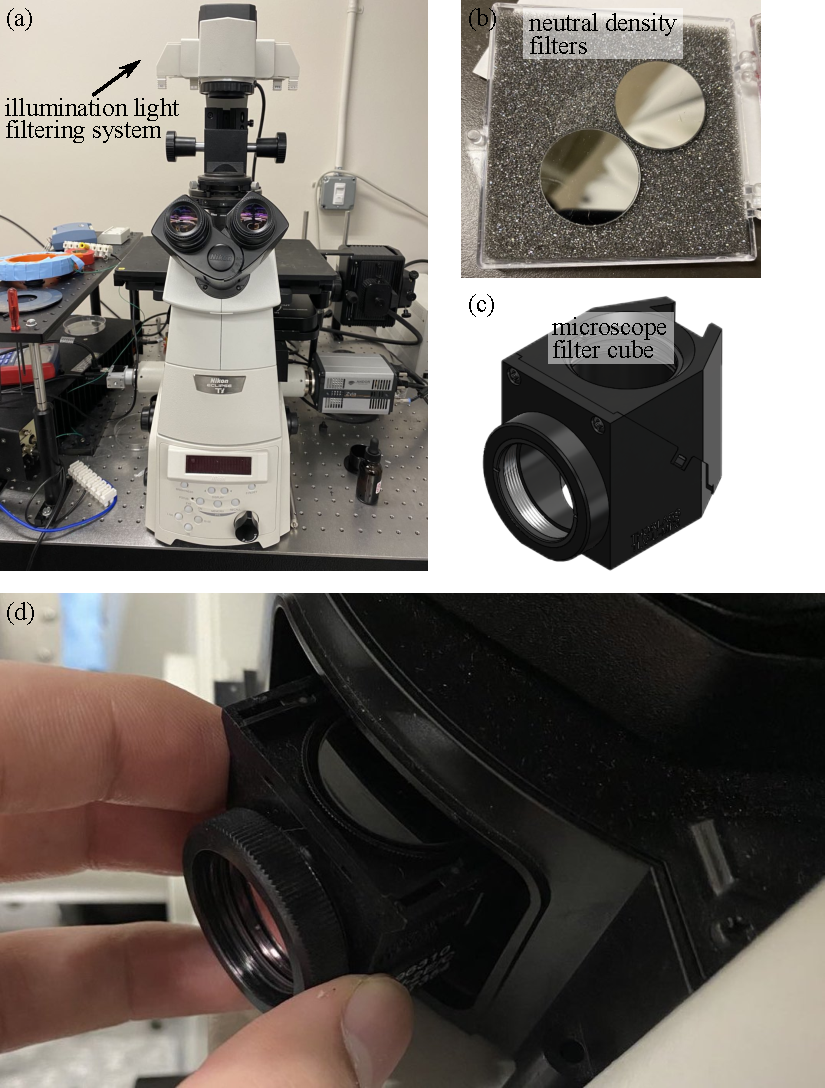
\includegraphics[width=4in]{figs/5-GNF/3.pdf}
\caption[Spatial and Temporal Correlation Functions in Active Turbulence]
{
\textbf{Spatial and temporal correlations functions of density and velocity in active turbulence.}
(a) Two-point density correlations at different bacterial volume fractions $\phi$. Radial position $r$ is normalized by the average length of bacteria $l_b = 3$ $\mu$m.
(b) Density autocorrelations at different $\phi$. Time $t$ is normalized by the characteristic swimming time of bacteria $\tau_b = 0.2$ s.
(c) Two-point velocity correlations at different $\phi$.
(d) Velocity autocorrelations at different $\phi$. $\phi$ ($\%$) of different curves are indicated in (a).
(e) Density and velocity correlation lengths, $\lambda$, versus $\phi$.
(f) Density and velocity correlation times, $\tau$, versus $\phi$.
The error bars in (e) and (f) represent the standard deviations of measurements over 3 independent experiments.
}
\label{fig:spatiotemporal-correlations}
\end{center}
\end{figure}

The correlation length $\lambda$ and correlation time $\tau$ are determined when the corresponding normalized correlation functions decay to $1/e$ (Fig.~\ref{fig:spatiotemporal-correlations}c, f). Fig.~\ref{fig:spatiotemporal-correlations}c shows the density correlation lengths at different $\phi$, which characterize the scale of density inhomogeneities in suspensions.
$\lambda$ is small at low $\phi$, gradually increases with $\phi$ and reaches a plateau of $\sim 5l_b$ in high-concentration bacterial suspensions of $\phi > \phi_c = 3.2\%$, where $l_b=3$ $\mu$m is the average length of bacterial body. The velocity correlation length follows the exact same trend and also saturates when $\phi > \phi_c$. Such a quantitative similarity indicates the direct coupling between density fluctuations and collective turbulent flows, a feature we shall examine in much more details later. In the fully-developed turbulent regime above $\phi_c$, the velocity correlation length is about twice of the density correlation length.
Fig.~\ref{fig:spatiotemporal-correlations}f shows the density and velocity correlation times at different $\phi$. The velocity and density correlation time at low $\phi$ show a large discrepancy. When $\phi > \phi_c=3.5\%$, they plateau at $\sim 6\tau_b$ and $\sim 4\tau_b$, respectively, where $\tau_b=0.2$ s is the characteristic time scale of \textit{E. coli} swimming.
% I don't know how to interpret the large difference in \tau at low concentration. It may be due to the dominanace of illumination light at low concentration.


\begin{figure}[!ht]
\begin{center}
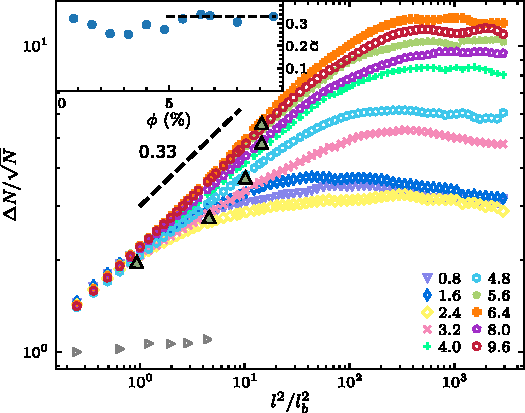
\includegraphics[width=4.5in]{figs/5-GNF/4.pdf}
\caption[Giant Number Fluctuations in Active Turbulence]
{
Density fluctuations of bacterial suspensions of different volume fractions $\phi$. The standard deviation of bacterial number $\Delta N$ in a subsystem of length $l$ as a function of the area of the subsystem $l^2$. $\Delta N$ is normalized by the length of the subsystem $l$, which is proportional to the square root of bacterial number in the subsystem $\sqrt N$. $l$ is presented in a dimensionless form, $\tilde{l} = l/l_b$, where $l_b = 3$ $\mu$m is the average length of bacteria. Dark green triangles indicate the density correlation lengths $\lambda(\phi)$ from Fig.~\ref{fig:spatiotemporal-correlations}e. The black dashed line indicates a power-law scaling of 0.33.
Inset: Scaling exponent $\alpha$ versus $\phi$. $\alpha$ are extracted by fitting the experimental data from 0.3$l_b$ to $\lambda(\phi)$. The dashed line in the inset indicates the theoretical prediction of $\alpha=1/3$.
}
\label{fig:GNF}
\end{center}
\end{figure}

We further examine GNF by calculating the standard deviation of bacterial number $\Delta N$ and the mean bacterial number $N$ in subsystems of increasing sizes. The normalized $\Delta N$ as a function of rescaled subsystem size $\tilde{l}^2=l^2/l_b^2$ for bacterial suspensions of different $\phi$ is plotted in Fig.~\ref{fig:GNF}, where $l$ is the side length of square subsystems.
Note that the area of the subsystem $l^2$ is linearly proportional to mean particle number $N$ at given $\phi$. At small length scale, when $l\le\lambda_n$, bacterial suspensions of all volume fractions examined in this study (0.8\% to 9.6\%) exhibit GNF, with $\Delta N$ increasing with subsystem size $l^2$. When the size of subsystems is much larger than the density correlation length $\lambda$, the giant fluctuation diminishes due to the spatial average over multiple dense and dilute regions.

The degree of GNF can be quantified by the scaling exponent $\alpha$ following $\Delta N/\sqrt{N} \sim N^\alpha$. $\alpha=0$ for equilibrium systems obeying the central limit theorem, whereas the upper bound $\alpha = 0.5$ corresponds to a system with maximal density fluctuations.
We extract $\alpha$ by fitting the experimental curves with power-law relations only below the density correlation length $\lambda$. The inset of Fig.~\ref{fig:GNF} shows $\alpha$ as a function of $\phi$.

At all volume fractions, $\alpha$ takes a value of $0.30 \pm 0.03$. Notably, at high volume fractions, when $\phi \geq \phi_h = 6.4\%$, $\alpha$ approaches a narrower plateau of $0.33 \pm 0.01$.

The plateau value quantitatively agrees with the theoretical prediction of $\alpha = 1/3$ for 3D suspensions of polar-ordered self-propelled particles with hydrodynamic interactions \cite{Simha2002}. As such, our experiments provide the first quantitative verification of the theory of GNF in 3D wet active fluids.

The observation of GNF at volume fractions lower than $\phi_c$ suggests that even in a dilute suspension below the turbulent transition, bacteria swim in a correlated fashion, in qualitative agreement with the prediction of the kinetic theory \cite{Stenhammar2017}.


\begin{figure}[!ht]
\begin{center}
\includegraphics[width=4.5in]{figs/5-GNF/5.pdf}
\caption[Energy Spectra in Active Turbulence]
{
Energy spectra $E(k)$ of bacterial suspensions of different volume fractions $\phi$. Shaded region indicates the range over which the scaling exponent $\beta$ is fitted. The black dashed line indicates a power-law scaling of $-3$. The red dashed line is a fitting of $E(k)$ at $\phi=0.8\%$ using Eq.~\ref{eq:energy-spectra}. In the fitting, the bacterial number density $n=\phi V_b$ and the dipole length $l_d = 1.9$ $\mu$m are from experiments, whereas the dipole strength $\kappa = 100$ $\mu$m$^3$/s and the regularization length $\epsilon = 14$ $\mu$m are taken as fitting parameters. In comparison, $\kappa = 300.8$ $\mu$m$^3$/s from experiments (see text).
Inset: Scaling exponent of $E(k)$, $\beta$, as a function of $\phi$. Dashed line indicates $\beta = 3.3$.
}
\label{fig:energy-spectra}
\end{center}
\end{figure}


\subsection{Energy Spectra}
Similar to GNF, the velocity field of active turbulence also shows scale-dependent structures, which are often characterized by the energy spectrum of turbulent flows, $E(k)$. $E(k)$ measures the kinetic energy density at different scales in terms of wavenumber $k = 2\pi/l$. It is related to the mean kinetic energy density by $\langle \bm{v}^2 \rangle/2 = \langle v_x^2 + v_y^2 \rangle/2 = \int_0^\infty E(k)dk$. Figure~\ref{fig:energy-spectra} shows $E(k)$ of bacterial suspensions at different $\phi$. In the dilute suspension of $\phi = 0.8 \%$, $E(k)$ is independent of $k$ in the small $k$ limit and then decreases at high $k$. The oscillation observed at high $k$ likely arises from PIV errors due to the small number of bacteria in each PIV box of low-$\phi$ suspensions. With increasing $\phi$, $E(k)$ at small $k$ increases sharply. In the turbulent regime at high $\phi$, the kinetic energy is concentrated at scales much larger than the size of single bacteria, even though the turbulent flow is entirely driven by the swimming of single bacteria. The overall trend of $E(k)$ with increasing $\phi$ qualitatively agrees with the results from large-scale particle simulations \cite{Saintillan2012,Bardfalvy2019}.

$E(k)$ of low-$\phi$ suspensions with uncorrelated pusher swimmers has been predicted \cite{Bardfalvy2019}
\begin{equation}
\label{eq:energy-spectra}
E(k) = 4\pi n \kappa^2 \left[ \frac{1}{3} + \frac{\cos(kl_d)}{(kl_d)^2} - \frac{\sin(kl_d)}{(kl_d)^3} \right] \frac{\epsilon^4k^2}{l_d^2} K_2^2(k\epsilon),
\end{equation}
where $n$ is the number density of bacteria, $\kappa$ is the dipole strength and $l_d$ is the dipolar length of \textit{E. coli}. $\epsilon$ is the distance for the regularization of the dipolar flow field. $K_2$ is the modified Bessel function of the second kind.
The fitting of Eq.~\ref{eq:energy-spectra} agrees well with our experimental $E(k)$ at low $\phi$ in the small $k$ limit (Fig.~\ref{fig:energy-spectra}). Particularly, Eq.~\ref{eq:energy-spectra} dictates that $E(k)$ is flat as $k \to 0$, a key feature confirmed by our experiments. A simple dimensional analysis can show that the plateau $E(k)$ at the small $k$ follows $\lim_{k \to 0}E(k) \sim n \kappa^2$ for uncorrelated swimmers of density $n$. The dipole strength can be estimated as $\kappa = Fl_d/\eta = \xi v_0 l_d/\eta = 300.8$ $\mu$m$^3$/s, where $\eta$ is the viscosity of the buffer. $\xi$ is the drag coefficient of a bacterial body orientated along its major axis, which can be calculated based on the body geometry $\xi = 3\pi\eta w_b \left[1-(1-l_b/w_b)/5\right]$ \cite{Magariyama2002}. $l_d = 1.9$ $\mu$m is taken from direct measurements \cite{Drescher2011}. Thus, $\lim_{k \to 0}E(k) \approx 7 \times 10^2$ $\mu$m$^3$/s, within the same order of magnitude of our experiments. The discrepancy between Eq.~\ref{eq:energy-spectra} and experiments at large $k$ may arise from the strong bacterial correlation at small length scales as shown by density fluctuations as well as the PIV errors.


We also extract the scaling exponent $\beta$ of $E(k) \sim k^{-\beta}$ by fitting the energy spectra at intermediate $k$, where a significant change of $E(k)$ with $\phi$ occurs and $E(k)$ exhibits good power-law relations. $\beta$ increases with $\phi$ and saturates around 3 at high $\phi > \phi_c$ (Fig.~\ref{fig:energy-spectra} inset). The saturated scaling exponent quantitatively agrees with previous experimental results obtained from the active turbulence of high-concentration sperm suspensions and \textit{B. subtilis} suspensions at large $k$ \cite{Creppy2015, Wensink2012}. At small $k$, $E(k)$ reported in Ref.~\cite{Wensink2012} decreases with decreasing $k$ and exhibits a non-monotonic trend, different from the result in this work. Such discrepancy is attributed to the confined geometry used in \cite{Wensink2012}, which limits the size of turbulent vortices and thus leads to a decrease of $E(k)$ at small $k$ \cite{Guo2018}. The large system size of $L = 140$ $\mu$m of our experiments allows us to probe the small $k$ limit predicted by theories and simulations without the influence of system boundaries.

Although the scaling in the small $k$ limit is strongly affected by the system size, the scaling in the large $k$ limit seems to be universal with $\beta \approx 3$ from different experiments. To the best of our knowledge, no theoretical prediction has been made on this universal scaling behavior for 3D active turbulence. Giomi investigated the energy spectra of 2D active nematics by combining numerical simulations with mean-field theories and showed $E(k) \sim k^{-4}$ in the large $k$ limit \cite{Giomi2015}.
The result has also been confirmed recently by a hydrodynamic theory \cite{Alert2020}. For isotropic turbulence in $d$ dimension, the energy spectra can be written as $E(k) = C_d k^{d-1} \langle \mathbf{v}(\mathbf{k})\cdot \mathbf{v}(-\mathbf{k})\rangle_{k = |\mathbf{k}|}$ \cite{Wensink2012,Bardfalvy2019},
where $C_d k^{d-1}$ is the surface area of $(d-1)$-sphere and $\langle \mathbf{v}(\mathbf{k})\cdot \mathbf{v}(-\mathbf{k})\rangle_{k = |\mathbf{k}|}$ is the Fourier transform of the velocity-velocity spatial correlation function. If the velocity correlation function for 2D active nematics is qualitatively similar to that of 3D bacterial suspensions independent of the dimensionality of systems, the mean-field theory would then predict a scaling of $E(k) \sim k^{-3}$, consistent with experimental observations. Such a hypothesis, although intriguing, is certainly non-trivial and needs further theoretical investigation.

\begin{figure}[!ht]
\begin{center}
\includegraphics[width=4in]{figs/5-GNF/6.pdf}
\caption[The Coupling between GNF and Kinetic Energy Spectra]
{
The coupling between density fluctuations and kinetic energies in the steady state.
(a) Energy spectra $E(k)$ plotted against number density fluctuations $\Delta N$ at each corresponding length scale for bacterial suspensions of different volume fractions $\phi$. Gray symbols are used for low-$\phi$ suspensions without active turbulence. The black dashed line is a polynomial fitting of the master curve, serving as a guide for the eye. The black arrow indicates the direction of increasing lengths.
(b) Correlation of local density fluctuations and kinetic energies $C$ as a function of $\phi$. $C$ is averaged over 1000 frames in steady state, and the error bars represent the standard deviations. Inset: Density fluctuation and kinetic energy fields in a bacterial suspension of $\phi = 4.8\%$.
}
\label{fig:GNF-energy-spectra-correlation}
\end{center}
\end{figure}


\subsection{Density-Flow Coupling}

Both GNF and energy spectra probe the scale dependence of active turbulence. The former measures density fluctuations at different scales, whereas the latter considers flow energies across scales. Although both properties have been extensively studied, the coupling between the two has not been explicitly examined so far.
The GNF curves and energy spectra shown in Fig.~\ref{fig:GNF} and \ref{fig:energy-spectra} show similar characteristics, including the rapid increase at small length scale and plateaus at large length scale. Such similarity suggests that a density-independent correlation between density fluctuations and kinetic energies may exist across all different length scales.
Indeed, when we plot density fluctuations $\Delta N$ against the corresponding kinetic energies $E$ at the same scale in Fig.~\ref{fig:GNF-energy-spectra-correlation}a, all the $\Delta N$-$E$ pairs fall onto a universal curve over two orders of magnitude in scales extending from the size of single PIV boxes to the vortex size in the turbulent regime, regardless of the specific volume fractions of the samples.
In contrast, $\Delta N$-$E$ shows much larger scattering for low $\phi$ suspensions with random swimming bacteria.
Although it is not surprising that density fluctuations correlate with kinetic energies in general as both measure different aspects of the same active turbulence, the collapse of data from samples of different volume fractions is still quite unexpected.
The results show that the coupling between density fluctuations and turbulent flows occur at every scale of active turbulence in a quantitative same fashion. Such a scale-invariant coupling is independent of the volume fraction of bacterial suspensions. A phenomenological fitting of the universal coupling between density fluctuations and kinetic energy is shown in Fig.~\ref{fig:GNF-energy-spectra-correlation}a by a black dashed line.

To further illustrate such an unusual coupling in real space, we measure the \emph{local} correlation of density fluctuations and kinetic energy at a randomly chosen small scale of $l = 2.5l_b$. The local density fluctuation $\delta N(\mathbf{r},t)$ and local kinetic energy $E(\mathbf{r},t)$ at position $\mathbf{r} = (x,y)$ and time $t$ are extracted from the image intensity field and the PIV velocity field, respectively (Fig.~\ref{fig:GNF-energy-spectra-correlation}b inset).
The normalized correlation between $\delta N(\mathbf{r},t)$ and $E(\mathbf{r},t)$ is then computed at different $\phi$ (Fig.~\ref{fig:GNF-energy-spectra-correlation}b). At low $\phi$ with random swimming bacteria, the correlation is weak fluctuating around zero, which then increases with $\phi$ as bacterial suspensions transition to active turbulence. A constant positive correlation is found in the turbulent regime when $\phi \geq \phi_c$. The real-space measurement provides a concrete example of the coupling between density fluctuations and turbulent flows at small scales.

\begin{figure}[!ht]
\begin{center}
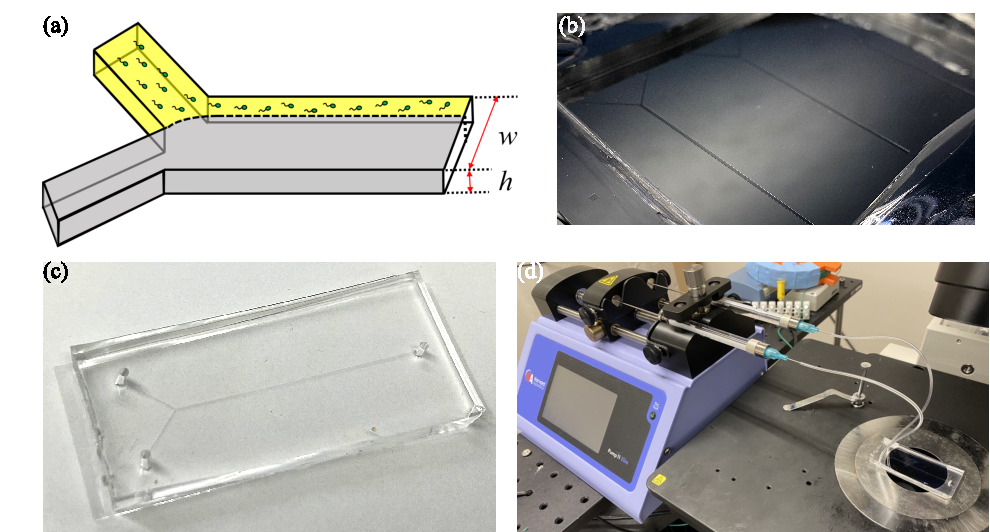
\includegraphics[width=4.5in]{figs/5-GNF/7.pdf}
\caption[Temporal Evolution of $\alpha$, Flow Kinetic Energy $\langle \bm{v}^2 \rangle/2$ and Fraction of Aligned Flow Region $M$]
{
\textbf{Temporal evolution of $\alpha$, flow kinetic energy $\langle \bm{v}^2 \rangle/2$ and fraction of aligned flow region $M$.}
(a) Snapshots of density fluctuation evolution during the transition towards active turbulence, overlaid with velocity fields obtained from PIV analysis. At $t=0$ s, we turn on the illumination light and the bacteria start to gain speed. Time are labeled in corresponding images ($\phi=6.4\%$).
(b) Temporal evolution of scaling exponent $\alpha$, total kinetic energy $E$ and the region fraction of aligned velocity $M$ in the same sample.
}
\label{fig:alpha-kinetics}
\end{center}
\end{figure}


Moreover, we find that the same density-energy coupling also exists in the kinetic process during the transition towards bacterial turbulence. Taking the advantage of the light-powered bacteria, we trigger the onset of bacterial turbulence by suddenly turning on the light illumination on high-$\phi$ bacterial suspensions at $t=0$ \cite{Peng2020}.
The temporal evolution of density fluctuations and turbulent flows in a bacterial suspension of $\phi = 6.4\%$ during the kinetic process is illustrated in Fig.~\ref{fig:alpha-kinetics}a. At $t=0$, the flow velocities are close to 0. The suspension shows no sign of density fluctuations. At $t=40$ s, although the magnitudes of velocities are still small, local alignment of velocity directions can be clearly observed, which gives rise to the characteristic pattern of vortices and jets of active turbulence. Weak density fluctuations start to emerge. At $t=103$ s, the magnitudes of velocities grow significantly and saturate. The suspension reaches the steady state of active turbulence with strong density fluctuations. Note that the response time of individual bacteria is much shorter than the emergence of collective flows. We provide Supplementary Moive S3 \cite{suppMovies} as a better visual illustration of this kinetic process.

\begin{figure}[!ht]
\begin{center}
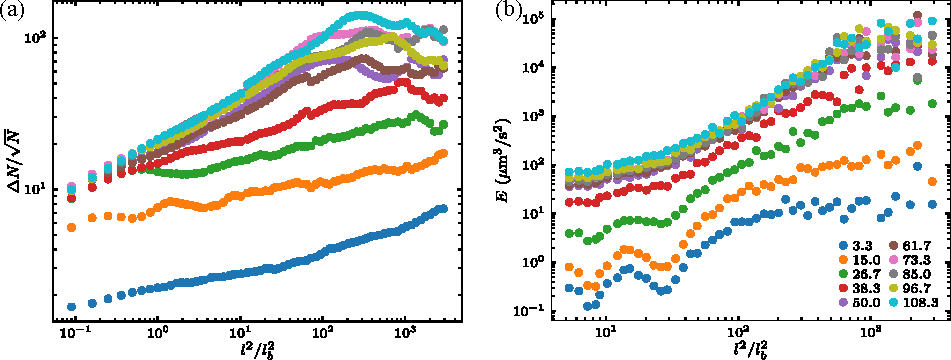
\includegraphics[width=5.5in]{figs/5-GNF/8.pdf}
\caption[Evolution of GNF and Energy Spectra during the Turbulent Transition]
{
\textbf{Evolution of GNF and energy spectra during the turbulent transition.} (a) Number density fluctuations $\Delta N$ and (b) energy spectra $E(k)$ as functions of subsystem size $l^2$ at different times over the turbulence transition of the same bacterial suspension. $\Delta N$ is normalized by the length of subsystems $l$, similar to that in Fig.~\ref{fig:GNF}. $\tilde{l} = l/l_b$. This particular sample has a volume fraction $\phi=6.4$. $t$ is indicated by the legends, in unit of seconds.
}
\label{fig:GNF-energy-spectra-kinetics}
\end{center}
\end{figure}

In Fig.~\ref{fig:alpha-kinetics}b, the evolution of the scaling exponent $\alpha$ is shown as a function of $t$. It grows relatively fast at the beginning and shows a saturation at $\sim 60$ s. The growth of both $\alpha$ and the large scale kinetic energy $\langle \bm{v}^2 \rangle/2$ are significantly delayed compared with the formation of collective flows, which is quantified by the area fraction of the regions with strong alignment of local velocities $M$ \cite{Peng2020}.
The finding provides strong experimental support to an important prediction of the kinetic theory of active fluids \cite{Saintillan2008a,Saintillan2008b}, where the density fluctuation arises due to the nonlinear coupling between collective flows and particle densities. At the onset of hydrodynamic instability in the linear regime, when velocities are largely aligned but flow strength is low, GNF is not very pronounced, as confirmed by our experiments at early times.

\begin{figure}[!ht]
\begin{center}
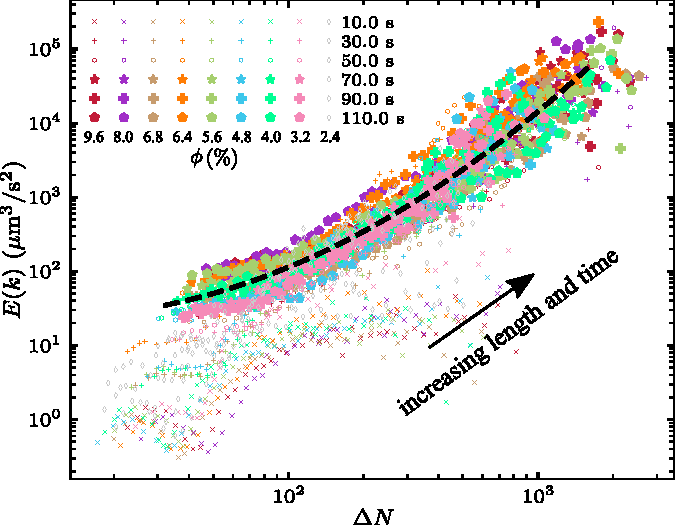
\includegraphics[width=4.5in]{figs/5-GNF/9.pdf}
\caption[Density Flow Coupling during the Transition towards Active Turbulence]
{
\textbf{Density flow coupling during the transition towards active turbulence.}
Kinetic energy $E(k)$ at various length scales is plotted against number fluctuations $\Delta N$ at corresponding length scales for bacterial suspensions at volume fractions ranging from 2.4\% to 9.6\% at different times. Different colors indicates samples of different volume fractions. The size and the shape of the markers indicate the time. Small markers stand for early times and large markers stand for late times. The black dashed line is the same master curve as shown in Fig.~\ref{fig:GNF-energy-spectra-correlation}a. In this plot, length scale and time are hidden variables, and their direction of evolving is indicated by a black arrow.
}
\label{fig:GNF-energy-spectra-correlation-transient}
\end{center}
\end{figure}

By comparing the temporal evolution of both GNF and energy spectra during the turbulence transition as shown in Fig.~\ref{fig:GNF-energy-spectra-kinetics}a and b, we find that they are analogous in at least two ways. First, both quantities reach a saturation at $\sim 60$ s. Second, both quantities grow faster at large length scales. Such analogies indicate that GNF and kinetic energy are  closely coupled not only in the steady state of active turbulence, but also during the transient state in the transition to active turbulence.
Motivated by this observation, we plot $\Delta N$ and $E(k)$ in the same axis for samples of different volume fractions, at different times and length scales in Fig.~\ref{fig:GNF-energy-spectra-correlation-transient}. Indeed, when $\phi>\phi_c$, all the data at different $t$, $\phi$ and length scale $l$ collapse into the same master curve obtained from the steady-state measurements. This kinetic measurements further suggest that the rise of GNF is governed by the kinetic energy at each corresponding scale.



\section{Conclusion}
We have conducted systematic experiments measuring density fluctuations and energy spectra of 3D bacterial suspensions over a wide range of concentrations in both steady and transient states. We illustrated the scaling behavior of giant number fluctuations in bulk bacterial suspensions and showed that such a scaling persisted at small scales even in low-concentration suspensions well before the transition to active turbulence. The finding provided new experimental evidence on the existence of local spatial and temporal correlations between bacteria in dilute suspensions due to the long-range hydrodynamic interactions unique to 3D wet active fluids. In addition, we also examined the energy spectra of bacterial suspensions of different concentrations and showed the spectral properties of the active turbulence of dense bacterial suspensions in the bulk limit. Lastly, by comparing density fluctuations and energy spectra at different scales, we revealed an unexpected coupling between density fluctuations and kinetic energies across more than one order of magnitude of length scales from the scale of single bacteria up to the size of the system. We further showed that such a density-independent and scale-invariant coupling also dominated the kinetic process during the transition towards bacterial active turbulence.

Our experiments also verified several important theoretical predictions on 3D wet active fluids:
\begin{enumerate}
\item The scaling behavior of density fluctuations observed in our experiments
$$
\Delta N/\sqrt N \sim N^{0.33}
$$
quantitatively agreed with the theoretical prediction on the giant number fluctuations of 3D suspensions of polar-ordered self-propelled particles \cite{Simha2002}.
\item The energy spectra of low-concentration bacterial suspensions measured in our study confirmed the key feature of the predicted energy spectra of uncorrelated pusher swimmers in the small wavenumber limit \cite{Bardfalvy2019}.
\item The delayed onset of density fluctuations uncovered in our experiments supported the central prediction of the kinetic theories on the nonlinear development of the hydrodynamic instability of pusher suspensions \cite{Saintillan2008a, Saintillan2008b}.
\end{enumerate}
Thus, our study provided a comprehensive experimental benchmark on the density fluctuations and energy spectra of bulk bacterial suspensions and shed new light onto the emergent dynamics of 3D wet active fluids.


% \chapter[The Emergence of Active Turbulence]{The Emergence of Active Turbulence\footnote[1]{
Reproduced in part with permission from (Yi Peng, Zhengyang Liu and Xiang Cheng, ``Imaging the emergence of bacterial turbulence using light-powered Escherichia coli'', \textit{arXiv e-print}).
}}
\label{the-emergence-of-active-turbulence}
%%%%%%%%%%%%%%%%%%%%%%%%%%%%%%%%%%%%%%%%%%%%%%%%%%%%%

\section{Introduction}
Collective motions of biological systems such as bird flocks, fish schools and bacterial swarms are the most vivid examples of the emergent behaviors of active matter \cite{Marchetti2013}. While moving independently at low density, self-propelled units in active matter can move collectively at high density, giving rise to coherent flows at length scales much larger than the size of individual units. In bacterial suspensions, these coherent flows exhibit a chaotic pattern of intermittent vortices and jets, reminiscent of turbulent flows at high Reynolds numbers. Hence, the flows induced by bacterial collective swimming are also known as active or bacterial turbulence \cite{Wolgemuth2008, Wensink2012, Linkmann2019, Dunkel2013}.
Extensive theoretical and numerical studies have been conducted in understanding the physical principles underlying the nonequilibrium transition between the disordered and the turbulent states in bacterial suspensions \cite{Marchetti2013, Ramaswamy2010, Koch2011, Saintillan2015}.
Particularly, kinetic theories have been developed by extending the classic models of suspensions of passive rod-shaped particles \cite{Koch2011, Saintillan2015, Stenhammar2017}. The theories consider the probability distribution of the position and orientation of bacteria based on a Smoluchowski equation, where a bacterium is modeled as a rigid rod exerting a pusher-type force dipole on the suspending fluid. In addition to self-propulsion, the motion of bacteria is further coupled with a mean-field background Stokes flow, driven by an average active dipolar stress as well as more conventional particle-induced viscous stresses.
Using the kinetic theories, Saintillan and Shelley first showed that a long wavelength hydrodynamic instability drives the transition to active turbulence in suspensions of pusher swimmers \cite{Saintillan2015, Saintillan2008a, Saintillan2008b, Hohenegger2010}.
The transition kinetics was further studied beyond the linear regime by numerically solving kinetic equations \cite{Saintillan2008b} and simulations of self-propelled rods \cite{Saintillan2012}.
By incorporating the effect of tumbling and rotational diffusion in the kinetic theories, Subramanian and Koch independently showed that the isotropic disordered state of bacterial suspensions becomes unstable above a threshold concentration in the bulk limit \cite{Koch2011, Subramanian2009}. The threshold concentration increases with the random reorientation and decreases with the swimming activity of bacteria. In general, the kinetic theories assume long-range hydrodynamic dipolar interactions between bacteria and are therefore strictly valid only for dilute suspensions. Nevertheless, the onset of bacterial collective swimming is typically observed at intermediate to high concentrations where steric interactions are supposed to be important \cite{Aranson2007, Ezhilan2013, Cisneros2011}, raising the question on the relative importance of hydrodynamic versus steric interactions in the formation of bacterial turbulence.
Indeed, simulations and models with steric interactions have also been developed, which successfully predicted the rise of collective motions both with hydrodynamic interactions \cite{Aranson2007, Ezhilan2013} and without \cite{Sambelashvili2007, Baskaran2010}.
Although steric interactions have been shown to play a leading role in bacterial collective swimming in 2D or quasi-2D systems such as Hele-Shaw cells with two confining walls \cite{Ishikawa2006, Nishiguchi2017} and bacterial monolayers on agar substrates \cite{Darnton2010, Zhang2010}, it is still far from clear what is the dominant interaction leading to bacterial turbulence in 3D suspensions.

In comparison with the theoretical development, definitive experiments on bacterial suspensions that can quantitatively verify theoretical predictions are still few and far between \cite{Koch2011, Saintillan2015}.
Pioneering experiments on suspensions of Bacillus subtilis first showed the emergence of bacterial turbulence at high concentrations in absence of bioconvection and chemotaxis \cite{Cisneros2011, Dombrowski2004, Cisneros2007, Sokolov2007, Sokolov2009}.
Various physical properties of bacterial turbulence such as density fluctuations \cite{Sokolov2009}, coherent and defect flow structures \cite{Sokolov2012, Ryan2013, Guo2018, Li2019} and mass and momentum transports \cite{Peng2016, Lopez2015, Liu2019, Yang2016} have been subsequently studied.
While most of these studies focused on the rise of bacterial turbulence with increasing bacterial concentrations, few experiments have considered other factors important for bacterial turbulence such as the swimming speed of bacteria \cite{Sokolov2012, Ryan2013} and the presence of defective immobile bacteria. A systematic mapping of the phase diagram of 3D bacterial flows over a large control parameter space is still lacking. Such an experimental phase diagram is essential to verify the quantitative prediction of the kinetic theories. Particularly, the study of the effect of doping immobile bacteria on the phase dynamics will provide strong evidence to resolve the controversy over the dominant interaction responsible for collective swimming in 3D suspensions of microorganisms \cite{Aranson2007, Ezhilan2013}. Increasing the ratio of immobile to mobile bacteria in a suspension of fixed total bacterial concentration would proportionally reduce the active stress and thus suppress the hydrodynamics-driven collective motion. On
the contrary, adding immobile bacteria to a suspension with a fixed concentration of mobile bacteria would promote steric interactions due to the rigid rod-shaped body of immobile bacteria and therefore enhance the collective motion if steric interactions are the leading cause of bacterial turbulence.

Moreover, the kinetic pathway towards the collective motion of swimming microorganisms remains largely unexplored. The kinetics of a phase transition affects both the transition rate and the structure of intermediate states and is of importance in understanding the phase dynamics of equilibrium systems \cite{Peng2015}. It plays a key role in distinguishing first-order and second-order phase transitions. Kinetics is equally important in a nonequilibrium phase transition, which can reveal not only the nature of the transition but also the missing link between the rise of the macroscopic order and the microscopic interparticle interaction. Hence, resolving the route to bacterial turbulence---a premier example of collective motions---addresses the central question in active matter: how do random self-propelled units self-organize into large-scale dynamic structures?

Here, we aim to address the above open questions. Our experiments provide not only the most comprehensive phase diagram of the flow of 3D bacterial suspensions heretofore, but also the detailed characterization of the kinetic route of the bacterial turbulent transition. Our experimental phase diagram quantitatively agrees with the kinetic theories, as well as our simple hydrodynamic model balancing dipolar interactions and rotational diffusion of bacteria. By further examining the effect of doping immobile bacteria on the phase dynamics, we show unambiguously that hydrodynamic interactions dominate the formation of collective swimming in 3D bacterial suspensions. Moreover, our kinetic measurements reveal an unexpected kinetic pathway near the phase boundary in analogy of the nucleation and growth process in equilibrium phase transitions and confirm the existence of a long-wavelength instability deep inside the turbulent phase. Together, our experiments validate the basic assumption of the kinetic theories and corroborate the principal predictions of the theories on the transition point and the mode of instability. Furthermore, our study uncovers new kinetic features of the bacterial turbulent transition and sheds new light on the nature of the nonequilibrium phase transition in active microbiological systems. These findings open new questions for future experimental and theoretical development.

\begin{figure}[!ht]
	\begin{center}
	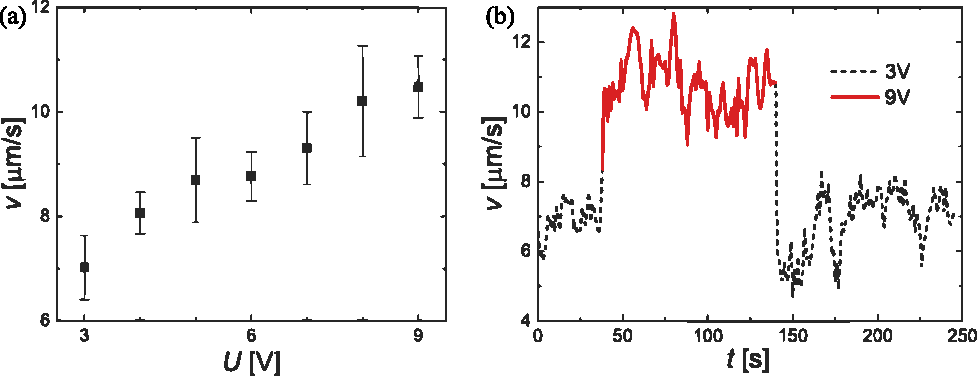
\includegraphics[width=5.5 in]{Figs/4-Emergence/S1.pdf}
	\end{center}
	\caption[Motility of light-powered bacteria]
	{
	\textbf{Motility of light-powered bacteria.}
  (a) Swimming speeds of the light-powered bacteria at different light intensities.
  The light intensity is tuned by setting the voltage of the illuminating lamp from 3 V up to 9 V.
  The average swimming speeds and the error bars are obtained by measuring tens of bacteria at a low bacterial volume fraction of $\phi=1.8\times 10^{-4}$ away solid boundaries. The measurements are taken 2 min after setting the light intensity, sufficient for the motility of bacteria reaching the steady state.
  (b) Temporal evolution of bacterial speed when the light intensity is changed.
  The velocity is averaged over all the bacteria in the field of view within a time interval of 1 s ($\sim 100$ bacteria).
  The video is taken at 30 frames per second. The response of bacteria to the change of light is fast on the order of seconds.
	}
	\label{fig:4-motility}
\end{figure}



\section{Methods}

\subsection{Bacteria}
Three strains of \textit{Escherichia coli} (\textit{E. coli}) are used. (i) A wild-type \textit{E. coli} K-12 strain (BW25113), which executes normal run-and-tumble motion with an average swimming speed $v = 28.7$ $\mu$m/s \cite{Berg2004}. (ii) A ``tumbler'' strain, which is made by knocking out $cheZ$ of a wild-type \textit{E. coli} strain (RP1616). The $\Delta cheZ$ mutant shows constant tumbling motions. We use tumblers as passive particles. To deactivate the bacteria, we remove the flagella of tumblers by pipetting tumbler suspensions through a narrow pipette tip a few tens of times. (iii) A light-powered \textit{E. coli}, whose swimming speed can be reversibly controlled by light. We introduce a light-driven transmembrane proton pump, proteorhodopsin (PR), to wild-type \textit{E. coli} (BW25113) by transforming the bacteria with plasmid pZE-PR encoding the SAR86 $\gamma$-proteobacterial PR-variant \cite{Walter2007}. The activity of PR is directly correlated with the light intensity. Thus, we can control the swimming speed of bacteria using light of different intensities.
The quantitative relation between the light intensity (in terms of the power of the light source) and the average swimming speed of bacteria is measured by tracking the motion of bacteria in dilute suspensions (Fig.~\ref{fig:4-motility}a).
The response time of the bacteria is fast within a few seconds after the change of the light (Fig.~\ref{fig:4-motility}b).
Note that the highest speed of the light-powered bacteria at high light intensity is about 10 to 11 $\mu$m/s (Fig.~\ref{fig:4-turbulence}c), which is smaller than that of the wild-type strain.
Three strains share a similar body plan with the length of the bacterial body $2a = 2.8 \pm 0.4$ $\mu$m and the radius of $b = 0.5 \pm 0.2$ $\mu$m based on direct imaging of bacteria, where the errors are the standard errors of the measurements.

All the three strains are cultured using a similar procedure. They are first cultured at 37.0 °C with a shaking speed at 250 rpm for 14-16 hours in terrific broth (TB) culture medium. The saturated culture is then diluted 1:100 in TB culture medium and grown at 30 °C for 6.5 hours. PR expression is triggered by 1 mM isopropyl $\beta$-D-thiogalactoside and 10 $\mu$M methanolic all-trans-retinal, which are supplemented in the mid-log phase for the synthesis of proteorhodopsin. The bacteria are harvested by gentle centrifugation (800g for 5 min) in the late log phase. After discarding the supernatant, we resuspend bacteria
with motility buffer MB (0.01 M potassium phosphate, 0.067 M NaCl, 10 M EDTA, pH 7.0). The suspension is finally washed twice and adjusted to the target volume fraction. Note that the volume fraction of bacteria at the standard concentration of $n_0$ is $\phi = 0.0018$, where $n_0 = 8 \times 10^8$ cells/ml is the \textit{E. coli} concentration at $OD_{600} = 1.0$. To create the mixture of tumblers and swimmers, we separately prepare suspensions of tumblers and swimmers both at the targeted volume fraction. We then mix the two suspensions at a predetermined ratio to control the fraction of active swimmers $f$.



\subsection{Sample preparation and video microscopy}
For the wild-type bacteria, oxygen is necessary to maintain the swimming of bacteria. We deposit a 2 $\mu$l wild-type bacterial suspension on a microscope coverslip, which forms a free suspension-air interface on the top. The droplet is millimetric in the lateral directions ($x$-$y$) normal to the imaging plane and about 150 $\mu$m in height ($z$). The coverslip and the suspension are further enclosed in a humid chamber of $\sim 1000$
mm$^3$ to reduce evaporation as well as perturbation due to ambient air flows. An inverted microscope is used to image bacterial motions 70 $\mu$m above the coverslip, where the effect of oxygen gradients is weak and bacterial activity is uniform. No system-wide persistent flow associated with aerotaxis is observed in our experiments. The microscopy videos show bacterial flows in the 2D $x$-$y$ plane inside the 3D suspension (Supplementary Movie S2 \cite{suppMovies}).

For the light-powered bacteria, it is important to shut down the metabolic pathway of aerobic respiration, so that the locomotion of bacteria is solely controlled by the PR pump. We inject a suspension of light-powered bacteria into a sealed cell of $18 \times 3 \times 0.17$ mm$^3$. For concentrated bacterial suspensions above $\phi = 0.062$, bacteria stop swimming after a few minutes in the cell due to the depletion of oxygen. Microscope illumination is then used to switch on/off and control the activity of the PR pump for bacterial swimming. 2D bacterial flows are imaged 80 $\mu$m above the bottom wall.

For most of our experiments, 2D flow fields are imaged through an inverted bright-field microscope using a 10X (NA 0.3), 20X (NA 0.5) or 40X (NA 0.6) objectives. The field of view of images ranges from $640 \times 640$ $\mu$m$^2$ to $160 \times 160$ $\mu$m$^2$. To measure the velocity orientational order and the kinetic energy in steady states, one-minute videos are taken 15 minutes after wild-type \textit{E. coli} samples are loaded or 2 minutes after a new light condition is applied to lightpowered \textit{E. coli} samples. These times are sufficient for the sample to reach the steady state. Five-minute videos are taken for transition kinetics after light ramping. All the videos are recorded at 30 frames per second by a sCMOS camera. To control bacterial velocity, light intensity is tuned by the voltage of the light source. Three to twelve independent measurements are taken for each set of control parameters of our experiments.

To measure the dynamics of individual bacteria through the turbulent transition, we image fluorescent-labeled \textit{E. coli} with an inverted fast confocal microscope using a 60X objective (NA 1.4). The green fluorescent protein expressed in bacteria is excited by a 488 nm laser. The field of view of the images is $180 \times 120$ $\mu$m$^2$. Bacterial flows are imaged 10 $\mu$m above the coverslip. Five-minute videos are taken at 10 frames per second.

\subsection{Image processing and data analysis}
The velocity field of bacterial suspensions is obtained from raw videos using standard Particle Imaging Velocimetry (PIV). For each pair of neighboring frames, the interrogation window size shrinks from $19.2 \times 19.2$ $\mu$m$^2$ to $4.8 \times 4.8$ $\mu$m$^2$ in three iterations \cite{Scarano2001}. The final lattice spacing of the velocity field is 2.4 $\mu$m. The velocity field in Fig.~\ref{fig:4-turbulence}a shows the velocity vectors of every other lattices. To verify the accuracy of PIV,
we have also measured the dynamics of bacterial suspensions using Particle Tracking Velocimetry (PTV) on passive colloidal tracers embedded in bacterial suspensions. The PTV results qualitatively agree with the PIV findings on both phase boundary and transition kinetics.

Energy spectra quantify the energy distribution over different length scales, $\lambda = 2\pi/k$, where $k$ is the wavenumber. To obtain energy spectra, we first calculate the Fourier transform of the 2D velocity field $v_x(x,y)$ and $v_y(x,y)$ to obtain $u_k(k_x,k_y)$ and $v_k(k_x,k_y)$. The point-wise kinetic energy density in the k-space is then computed $E(k_x, k_y) = \langle u_k(k_x, k_y)u^*_k(k_x, k_y)+v_k(k_x, k_y)v_k^*(k_x, k_y)\rangle/2$, where $*$ represents the complex conjugate. Finally, the energy
spectrum $E(k)$ is obtained by summing up $E(k_x,k_y)$ at a constant $k=(k_x^2+k_y^2)^{1/2}$. An alternative way to calculate $E(k)$ through the Fourier transform of the two-point velocity correlation function $\langle \vec{v}(\vec{r_0})\cdot\vec{v}(\vec{r_0}+\vec{r})  \rangle_{\vec{r_0}}$ yields quantitatively similar results.

To extract bacterial nematic order, we perform Fast Fourier transformation (FFT) on the local regions ($20 \times 20$ $\mu$m$^2$) of confocal images.
The FFT patterns are first smoothed with 3 neighboring pixels (0.15 $\mu$m$^{-1}$) and then fitted with ellipses. The aspect ratio of the ellipses, $a/b$, quantifies the local nematic order of bacteria (Fig.~\ref{fig:4-microscopic}B inset).
The average of the aspect ratio is finally taken over the whole field of view, $F = \langle a/b \rangle$. To calibrate our method, we show numerically that the anisotropy of the FFT pattern of local regions, $a/b$, is approximately linearly proportional to the local nematic order parameter of bacteria $S=\frac{1}{N}\sum_{j=1}^N(3\cos^2\alpha_j - 1)/2$ within the range of our experiments, where $\alpha_j$ is the angle between the orientation of bacterium $j$ with respect to the mean orientation of all the $N$ bacteria in a local region in 3D.

\begin{figure}[!ht]
	\begin{center}
	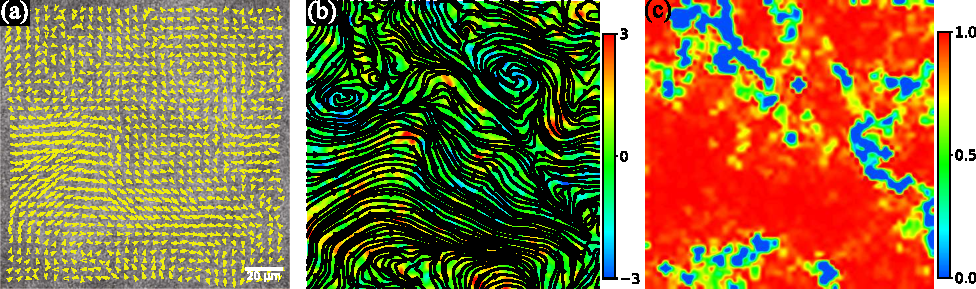
\includegraphics[width=5.5 in]{Figs/4-Emergence/1.pdf}
	\end{center}
	\caption[Bacterial turbulence]
	{
	\textbf{Bacterial turbulence.}
  (A) The flow field of a suspension of wild-type \textit{E. coli} at volume fraction $\phi=0.14$. The arrows indicate local velocities from PIV. Scale bar: 20 $\mu$m.
  (B) The corresponding streamlines and the vorticity field ($\omega$), highlighting the characteristic features of bacterial turbulence including intermittent jets and vortices (see also Supplementary Movie S2 \cite{suppMovies}).
  (C) The corresponding velocity orientational correlation field $c$. The area fraction of red regions with $c \ge 0.9$, $M$, is used to quantify the transition to bacterial turbulence. $M < 1$ even for this highly turbulent state due to the presence of vortex cores and interstices.
	}
	\label{fig:4-turbulence}
\end{figure}

\section{Results}

We use  \textit{E. coli} as our model bacteria. In order to examine a large control parameter space, three different strains of \textit{E. coli} are used in our experiments, which all share similar body plans (Methods). In addition to a wild-type strain (BW25113), a strain of tumblers with $cheZ$ knocked out (RP1616) and flagella removed is used as immobile passive bacteria. Moreover, a light-powered
\textit{E. coli} strain (BW25113 with proteorhodopsin, a light-driven transmembrane proton pump \cite{Walter2007}) is also used, whose motility can be varied by green light of different intensities (Fig.~\ref{fig:4-motility}). By mixing different strains of bacteria and controlling light intensity, we explore the phase diagram of 3D bacterial flows spanned by bacterial volume fraction $\phi$, the average swimming speed of bacteria $v$ and the number fraction of active swimmers $f$.

\begin{figure}[!ht]
	\begin{center}
	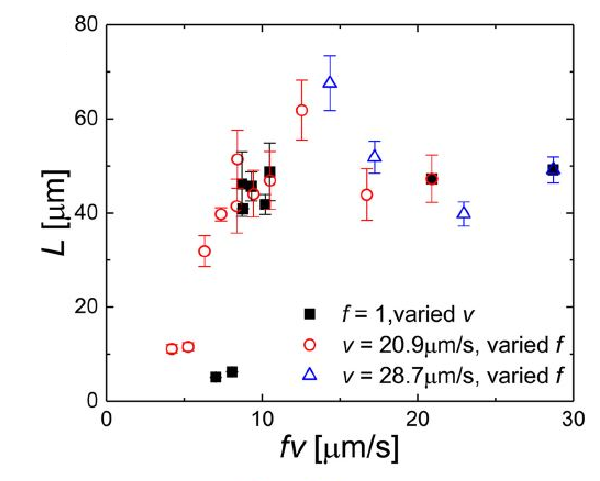
\includegraphics[width=4 in]{Figs/4-Emergence/S2C.pdf}
	\end{center}
	\caption[The correlation length as a function of the product of swimmer fraction and swimming velocity]
	{
	The correlation length $L$ as a function of the product of swimmer fraction and swimming velocity $fv$.
  }
	\label{fig:4-correlation-length}
\end{figure}

\subsection{Transition to bacterial turbulence}
The collective motion of bacteria leads to bacterial turbulence with characteristic intermittent jets and whirls, whose lengths and speeds are much larger than those of individual bacteria (Figs.~\ref{fig:4-turbulence}a, b and Supplementary Movie S2 \cite{suppMovies}). To quantify bacterial turbulence, we calculate the orientational correlation of local velocities, $c_i=\min_{j=1..4}(\hat{v_i}\cdot\hat{v_j})$, where $\hat{v_i}$ is the unit vector along the direction of the local velocity at position $i$ and $\hat{v_j}$ is the direction of the velocity in one of its four neighboring boxes adopted in Particle Imaging Velocimetry (PIV).
Note that our PIV measures 2D in-plane flows $\vec{v}=(v_x, v_y)$ in 3D bacterial suspensions (Methods). We identify a local region with high velocity orientational correlation when $c \ge 0.9$. The area fraction of these highly correlated regions, $M$, is used in our study as the order parameter quantifying the rise of bacterial turbulence (Fig.~\ref{fig:4-turbulence}c). This choice is similar to that used in previous studies \cite{Cisneros2011}. In addition to the velocity orientational order, we also measure the strength of bacterial flows via kinetic energy per unit mass, $E=\langle v_x^2 + v_y^2 \rangle / 2$.
Although the definition of kinetic energy density is the same as that used for classical turbulent flows, the inertia of bacterial swimming in our experiments is negligible with the Reynolds number on the order of $10^{-4}$.

\begin{figure}[!ht]
	\begin{center}
	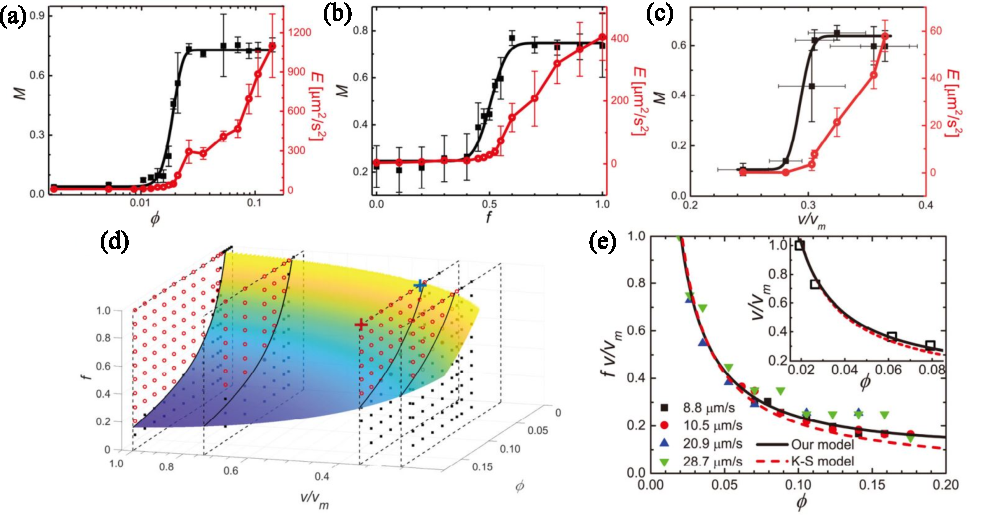
\includegraphics[width=5.5 in]{Figs/4-Emergence/2.pdf}
	\end{center}
	\caption[Transition to bacterial turbulence and the phase diagram of 3D bacterial flows]
	{
	\textbf{Transition to bacterial turbulence and the phase diagram of 3D bacterial flows.}
   (a) Velocity orientational order $M$ and kinetic energy $E$ as a function of bacterial volume fraction $\phi$ of wild-type bacteria with swimming speed $v_m = 28.7$ $\mu$m/s and swimmer fraction $f = 1$. Black squares are for $M$ and red circles are for $E$.
   (b) $M$ and $E$ versus $f$ at fixed $\phi= 0.053$ and $v = v_m$.
   (c) $M$ and $E$ versus $v$ at $\phi = 0.11$ and $f = 1$. $v$ is normalized by the swimming speed of wild-type bacteria $v_m$. Black lines indicate error function fittings. Each data point in (a)-(c) represent one experiment averaged over 30 s in time. The error bars are the standard deviations of the temporal fluctuations of measured quantities. The error bars in $v$ are the standard deviations of the natural variation of bacterial swimming speeds in the dilute limit. Although for clarify we only show one set of experiments for each case, we have run more than 20 independent experiments near the phase boundary to locate the transition points.
   (d) A phase diagram of bacterial flows in the phase space spanned by $\phi$, $v$ and $f$. Red circles indicate the turbulent phase, whereas black squares indicate the disordered phase. The surface is the model prediction (Eq.~\ref{eq:4-model}). The crosses indicate the locales of the kinetics experiments shown in Fig.~\ref{fig:4-kinetics} and \ref{fig:4-spectra}.
   (e) The rescaled phase boundary between the disordered and the turbulent phases at different $v$ (indicated in the figure). The black line is our model prediction (Eq.~\ref{eq:4-model}), whereas the red dashed line is the prediction of Koch and Subramanian (Eq.~\ref{eq:4-koch-model}). Inset shows the experimental phase boundary and the theoretical predictions with $f = 1$.
	}
	\label{fig:4-transition}
\end{figure}

A transition to bacterial turbulence is observed as we increase bacterial volume fraction, $\phi$ (Fig.~\ref{fig:4-transition}a). A sharp increase of $M$ occurs around $\phi = 0.018$. The transition point, $\phi_c$, is then obtained from the inflection point of the error function fitting of $M(\phi)$. The transition to bacterial turbulence at $\phi_c$ is also coincident with a more gradual increase of $E$ (Fig.~\ref{fig:4-transition}a).
We find similar sharp transitions to bacterial turbulence when increasing $v$ and $f$ at fixed $\phi$ (Fig.~\ref{fig:4-transition}b, c).
Particularly, bacterial turbulence is observed at $f = 20\%$ for the mixture of wild-type \textit{E. coli} ($v = 28.7$ $\mu$m/s) and immobile bacteria at $\phi = 0.18$. Such a low $f$ demonstrates the robustness of the collective flow of bacterial suspensions, greatly surpassing the state-of-the-art design of active robotic systems \cite{Li2019a}.
This high tolerance to malfunctioning units likely arises from long-range hydrodynamic interactions, lacking in dry active matter \cite{Marchetti2013}.

\subsection{3D phase diagram}
Systematic measurements over a thousand bacterial samples under different combinations of control parameters yield a full 3D phase diagram of bacterial flows, where bacterial turbulence emerges at large $\phi$, $v$ and $f$ (Fig.~\ref{fig:4-transition}d).
It should be emphasized that, although the transition to bacterial turbulence has been investigated with increasing $\phi$ and $v$ in separate experiments \cite{Cisneros2011, Sokolov2007, Sokolov2009, Sokolov2012, Ryan2013}, to the best of our knowledge, systematic measurements over such a large parameter space in the same experimental system have not been achieved previously. This comprehensive 3D phase diagram not only allows us to quantitatively verify the theoretical prediction on the transition point, but also sets up a framework for exploring the kinetics of the transition in the next section.

We first estimate the phase boundary between disordered and turbulent phases using a simple hydrodynamic model proposed in Ref.~\cite{Drescher2011}, where the pairwise hydrodynamic interaction that promotes local bacterial alignment competes with the rotational relaxation that disorientates bacteria. Although these
two competing factors also form the basic ingredients of the kinetic theories \cite{Koch2011, Saintillan2015}, this simple model considers the interaction between two bacteria, instead of mean-field particle probability distributions. Specifically, we calculate the rotation of a bacterium in a flow field induced by the swimming of its neighbor at distance $r$. A critical distance $r_c$ is determined when the flow-driven rotation of the bacterium balances the reorientation of the bacterium due to random tumbling and rotational diffusion. The transition volume fraction is then given as $\phi_c=V_b/r_c^3$, where $V_b = 2\pi ab^2 = 2.20$ $\mu$m$^3$ is the volume of a single bacterium. Here, we approximate the bacterial body as a cylinder with an average length $2a = 2.8$ $\mu$m and
radius $b = 0.5$ $\mu$m. The volume of bacterial flagella is too small to be considered when calculating $V_b$. To incorporate the presence of immobile bacteria, we extend the original model and include the higher-order hydrodynamic interaction due to reflection flows in the calculation. The model predicts the transition concentration $\phi_c$ in the bulk limit
\begin{equation}
  \label{eq:4-model}
  \phi_c-\frac{r_0^3}{V_b}\phi_c^2 = \frac{v_0}{fv},
\end{equation}
where $r_0 = 1.6$ $\mu$m provides a characteristic interaction range of the reflection flows and $v_0$ is a velocity scale determined by the strength of the force dipole and the rotational relaxation of bacteria
$$
v_0 = \frac{8\pi\eta V_b}{\xi l (\Gamma+1)}\sqrt{\frac{20D_r}{3\tau}}
$$
Here, $\eta = 1$ mPa$\cdot$s is the viscosity of suspension buffer, $\xi = 1.91 \times 10^{-8}$ kg/s is the drag coefficient of bacterial body, $l = 1.9$ $\mu$m is the distance of the force dipole of bacteria and $D_r = 0.057 s^{-1}$ is the effective diffusion coefficient of bacteria. $\xi$, $l$ and $D_r$ are all obtained from direct experimental measurements \cite{Drescher2011}.
$\Gamma = (a^2-b^2)/(a^2+b^2)$ is the shape factor of a bacterial body.
Lastly, $\tau$ quantifies the interaction time of two bacteria bounded between $a/v \sim 0.1$ s and the average tumbling time $\tau_t \sim 1$ s \cite{Berg2004}. Direct fitting of the phase boundary yields $\tau = 0.85 \pm 0.04$ s within the bound, which leads to $v_0 = 0.57$ $\mu$m/s. Eq.~\ref{eq:4-model} allows for the collapse of the transition boundaries of different parameters and shows an excellent agreement with experiments (Fig.~\ref{fig:4-transition}e).
The rescaled phase boundary shows that the fraction of active swimmers couples with the velocity of bacteria in determining the transition to bacterial turbulence. The equivalence of $f$ and $v$ can be further seen from the dynamic structure of the turbulent flows beyond the transition point, where the velocity correlation length of bacterial flows at different $v$ and $f$ also collapses into a master curve when plotting against $fv$ (Fig.~\ref{fig:4-correlation-length}C). Thus, by varying $f$, we can effectively extend bacterial velocity over a much broader range in experiments.

The simple hydrodynamic model discussed above provides a physically intuitive picture for the emergence of bacterial collective motions. However, to incorporate many-body interactions beyond two bacteria and avoid the divergence associated with the slow algebraic decay of the dipolar interaction, one needs to consider effective media or averaged equations adapted in the kinetic theories \cite{Subramanian2009}. Next, we compare our experiments with the prediction of the kinetic theories. First, at low $\phi_c$, the higher order term on the left side of Eq.~\ref{eq:4-model} is negligible, which leads to $\phi_c \sim 1/v$, consistent with the kinetic theories \cite{Koch2011, Stenhammar2017, Bardfalvy2020}. Quantitatively, Koch and Subramanian predicted the transition volume fraction in the bulk limit \cite{Koch2011}
\begin{equation}
  \label{eq:4-koch-model}
  \phi_c = \frac{\eta V_b}{\xi l}\left[ \frac{5}{\tau_t} + 30D_r \right] \frac{1}{fv}
\end{equation}
where $\xi = 6\pi\eta b \left[ 1-\frac{1}{5}(1-\frac{a}{b}) \right] \approx 1.28 \times 10^{-8}$ kg/s is the calculated drag coefficient of bacterial body
orientated along its major axis, which is slightly smaller than the measured valve shown above. The linear stability analysis of the original kinetic theories can be easily extended for the mixture of mobile bacteria and immobile bacteria with zero dipolar strength \cite{Subramanian2009, Bardfalvy2020}, which results in $f$ as the prefactor of $v$ in Eq.~\ref{eq:4-koch-model}.
Without fitting parameters, Eq.~\ref{eq:4-koch-model} quantitatively agrees with our experiments (Fig.~\ref{fig:4-transition}e), although small deviations between the theory and experiments can be observed at high concentrations. As such, our systematic measurements of the phase diagram provide a quantitative verification of the prediction of the kinetic theories on the transition point.
Our experiments also confirm numerical results from large-scale particle-based simulations with hydrodynamic interactions and random reorientations \cite{Krishnamurthy2015, Bardfalvy2019}, where collective motions have been observed above the predicted threshold concentration.


\begin{figure}[!ht]
	\begin{center}
	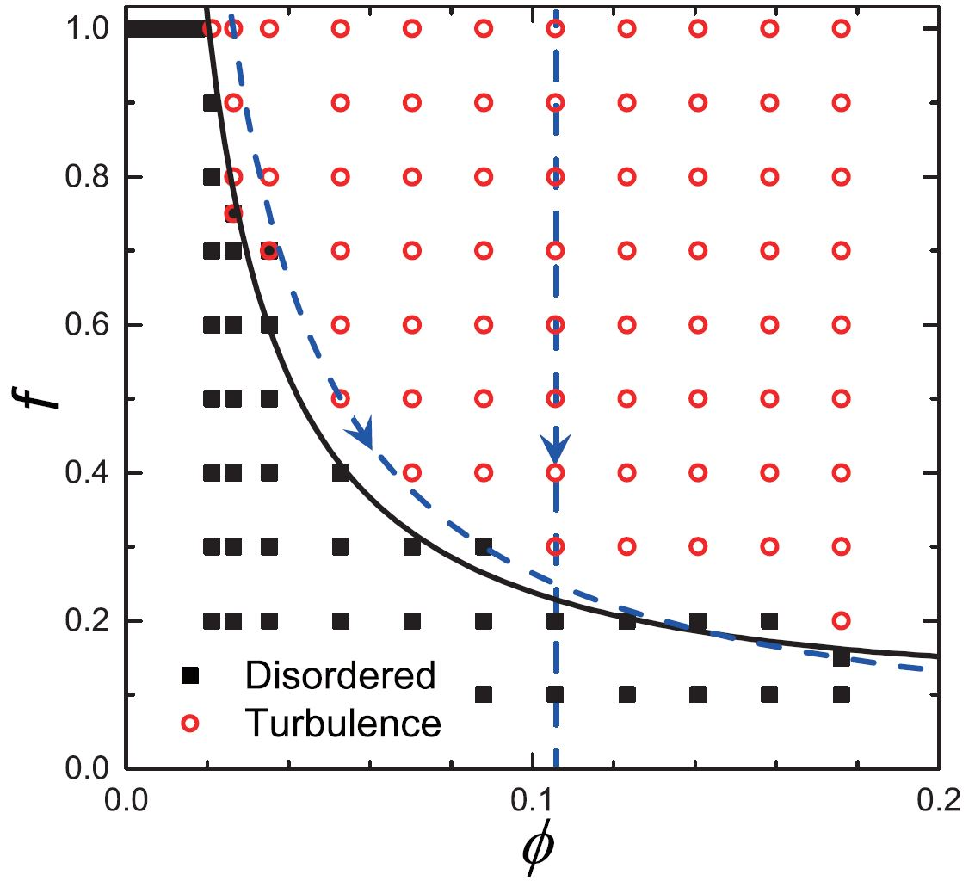
\includegraphics[width=4 in]{Figs/4-Emergence/S3.pdf}
	\end{center}
	\caption[Effect of immobile bacteria]
	{
	\textbf{Effect of immobile bacteria.}
  The phase diagram as a function of bacterial volume fraction $\phi$ and swimmer fraction $f$ at a fixed swimming velocity $v=28.7$ $\mu$m/s.
  Black squares indicate the isotropic disordered phase, whereas red circles indicate the turbulent phase.
  The black solid line represents the phase boundary predicted by our simple hydrodynamic model (Eq.~\ref{eq:4-model}).
  The vertical line indicates a constant total bacterial concentration $\phi=0.11$, whereas the curved dashed line indicates a constant concentration of active swimmers $\phi f = 0.027$.
  The arrows on the dashed lines show the direction of increasing the fraction of immobile bacteria $1 - f$.
	}
	\label{fig:4-immobile}
\end{figure}

At $f = 1$, we find $\phi_c$ ranges between 0.02 and 0.08 for different bacterial velocities (Fig.~\ref{fig:4-transition}e inset). The average distance between bacteria at $\phi_c$ is about 6 to 9.5 $\mu$m, on the order of the size of a single bacterium \cite{Berg2004}. Short-range hydrodynamic and steric interactions could be important at such small scales \cite{Aranson2007, Ezhilan2013}. Hence, it is nontrivial that the far-field dipolar hydrodynamic interaction adapted in our simple model (Eq.~\ref{eq:4-model}) and in the kinetic theories (Eq.~\ref{eq:4-koch-model}) is sufficient to describe the experimental phase boundary.
The observation supports the basic assumption of the kinetic theories \cite{Koch2011, Saintillan2015}. Consistent with this finding, increasing the fraction of immobile bacteria at either a fixed total bacterial volume fraction $\phi$ or a fixed volume fraction of active swimmers $f\phi$ suppresses bacterial turbulence in our experiments (Fig.~\ref{fig:4-immobile}), rather than promoting the collective motion as observed in dry active matter with purely short-range steric interactions \cite{Kumar2014}. Thus, our study provides experimental evidence on the dominant role of long-range hydrodynamic interactions in 3D suspensions, resolving the controversy over the interparticle interaction responsible for 3D bacterial collective swimming. Physically, if bacterial orientation is random, the effective volume occupied by a bacterium should be considered as a sphere of radius a instead of the excluded volume of the bacterial body Vb, which would lead to much larger effective $\phi_c$ up to 0.41 in the semi-dilute regime \cite{Cisneros2011}. The dominant role of the long-range dipolar interaction observed in our
experiments suggests that bacterial orientation is strongly correlated near the phase boundary under the influence of the hydrodynamic interaction. As a result, bacteria show preferred alignment with their neighbors, giving rise to relatively large inter-bacteria distances suitable for the long-range hydrodynamic interaction.

Lastly, it is worth noting that the size of samples in our experiments is fixed with the minimal dimension between 150 $\mu$m and 170 $\mu$m, much larger than the size of single bacteria. The volume of our samples is on the order of several microliters, which contains more than 107 bacteria at $\phi = 0.018$. Simulations and kinetic theories have shown that $\phi_c$ is independent of the system size at such large scales \cite{Stenhammar2017}. More recent experiments have also shown that the onset of collective motions and bacterial superfluids is insensitive to the system size above 170 $\mu$m \cite{Martinez2020}. Thus, the phase diagram shown in Fig.~\ref{fig:4-transition}d should approximate the phase behavior of bacterial suspensions in the bulk limit.


\begin{figure}[!htbp]
	\begin{center}
	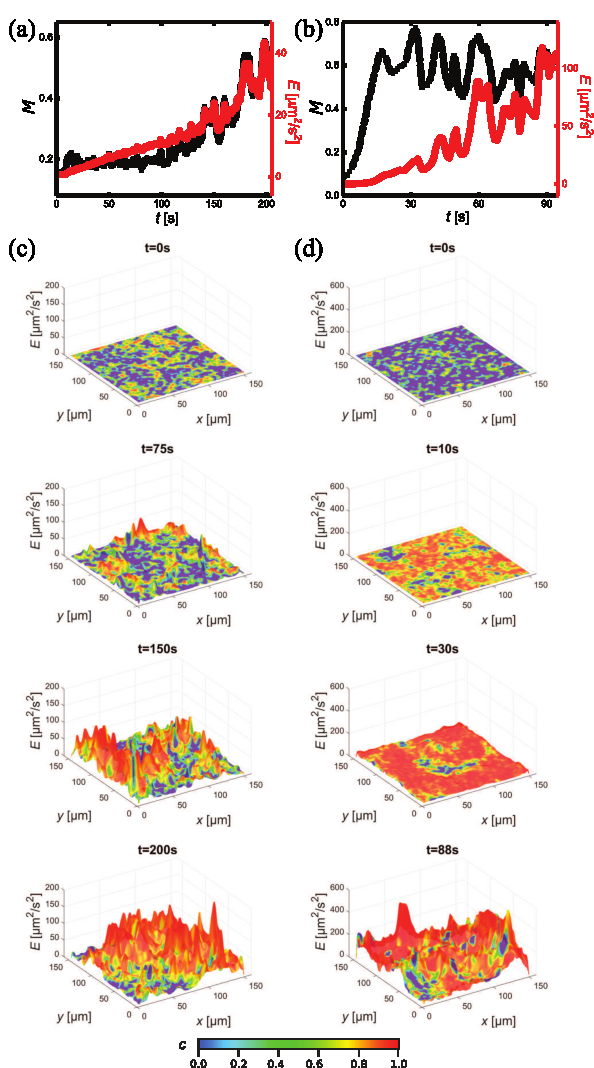
\includegraphics[height=5.2 in]{Figs/4-Emergence/3.pdf}
	\end{center}
	\caption[Transition kinetics]
	{
	\textbf{Transition kinetics.}
  (a) Velocity orientational order $M$ and kinetic energy $E$ as a function of time through the turbulent transition. $t = 0$ corresponds to the time when light intensity is ramped up. Bacterial volume fraction $\phi = 0.071$, speed $v = 10.5$ $\mu$m/s and swimmer fraction $f = 1$, which is near the phase boundary shown by the blue cross in Fig.~\ref{fig:4-transition}d.
  (b) Spatiotemporal evolution of the local velocity orientational correlation $c$ and the local kinetic energy $E$ over the transition shown in (a). The spatial coordinates are shown in the $x$-$y$ plane. The height indicates the value of $E$, whereas the color shows the value of $c$.
  (c) $M$ and $E$ as a function of $t$ for $\phi = 0.18$, $v = 10.5$ $\mu$m/s and $f = 1$ deep inside the turbulent phase shown by the red cross in Fig.~\ref{fig:4-transition}d (see also Supplementary Movie S2 \cite{suppMovies}).
  (d) Spatiotemporal evolution of $c$ and $E$ over the transition shown in (c).
	}
	\label{fig:4-kinetics}
\end{figure}



\subsection{Transition kinetics}
Next, using the phase diagram as a roadmap, we explore the kinetics of bacterial turbulent transition, which reveals the mode of instability and the transient structure of bacterial suspensions through the transition. To study the kinetics, we trigger the onset of bacterial turbulence by suddenly ramping up light intensity at $t = 0$, which increases the swimming speed of light-powered bacteria from that below the phase boundary to high $v$ above the boundary at a given combination of $\phi$ and $f$. Although individual bacteria in dilute suspensions recover their swimming speeds within a couple of seconds (Fig.~\ref{fig:4-motility}), the emergence of collective flows can take much longer times depending on the specific control parameters. In the region above but close to the phase boundary, the transition exhibits a surprisingly long incubation period with low velocity orientational order $M$ and kinetic energy $E$ ($\sim 100$ s in Fig.~\ref{fig:4-kinetics}a). During incubation, localized regions with relatively large velocity orientational correlation (high $c$) and large kinetic energy (high $E$) nucleate within the disordered phase (Fig.~\ref{fig:4-kinetics}b).

The incubation period witnesses the slow growth and the fluctuation of these high-$c$ and high-$E$ regions. After incubation, the high-$c$ and high-$E$ regions grow quickly and eventually percolate the entire system.
$M$ and $E$ are directly coupled and increase simultaneously during the transition. The incubation period becomes increasingly short as we move away from the phase boundary.
Far above the boundary, the increase of the velocity orientational correlation is almost instantaneous across the entire system after the light ramp (Fig.~\ref{fig:4-kinetics}c, d and Supplementary Movie S2 \cite{suppMovies}), whereas the kinetic energy remains low at beginning and grows to a steady-state plateau only at a later time.
The growths of $M$ and $E$ are decoupled in this case.
The system exhibits a transient state with high velocity orientational order but low kinetic energy (the middle two pictures at $t = 10$ and $30$ s in Fig.~\ref{fig:4-kinetics}d).

\begin{figure}[!htbp]
	\begin{center}
	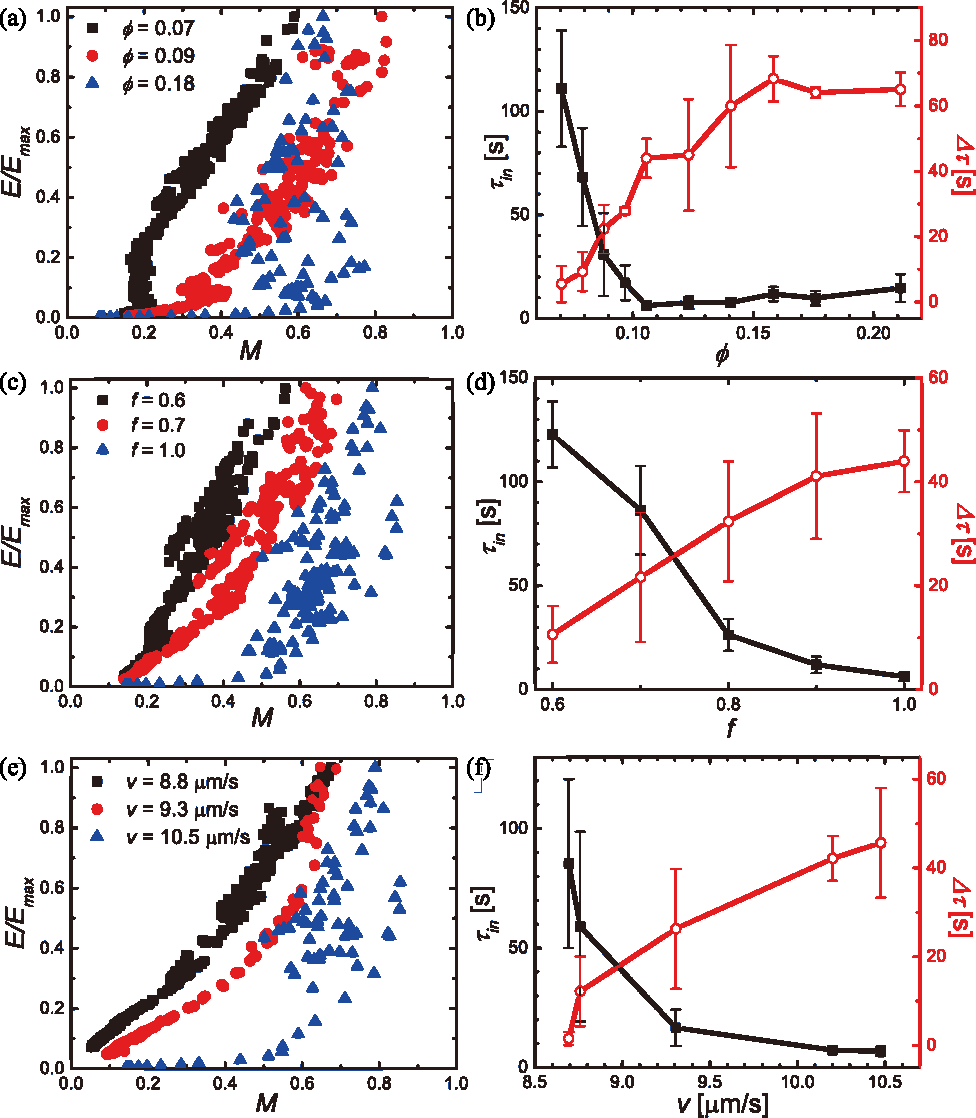
\includegraphics[height=5 in]{Figs/4-Emergence/4.pdf}
	\end{center}
	\caption[One-step and two-step transitions]
	{
	\textbf{One-step and two-step transitions.}
  (a) Kinetic energy $E$ versus velocity orientational order $M$ over a transition at a given bacterial volume fractions $\phi$, fixed bacterial speed $v = 10.5$ $\mu$m/s and swimmer fraction $f = 1$. While the one-step transition shows an approximately linear concurrent increase of $E$ and $M$ over time (black squares), the two-step transition shows an increase $M$ at low in the first step at early times and then an increase of $E$ at an approximately constant $M$ in the second step at later times (blue triangles). $E$ is normalized by the maximal energy density at the steady state, $E_{max}$.
  (b) Incubation time, $\tau_{in}$, and the time difference, $\Delta\tau$, as a function of $\phi$ at the same $v$ and $f$ as in (a). The error bars reflect the standard error of three to twelve experimental runs for each data point.
  (c) $E/E_{max}$ versus $M$ at different $f$ and a fixed $\phi= 0.11$  and $v = 10.5$ $\mu$m/s.
  (d) $\tau_{in}$ and $\Delta\tau$ at different $f$ at the same $\phi$ and $v$ as in (c).
  (e) $E/E_{max}$ versus $M$ at different $v$ and a fixed $\phi= 0.11$  and $f = 1$.
  (f) $\tau_{in}$ and $\Delta\tau$ at different $v$ at the same $\phi$ and $f$ as in (e).
	}
	\label{fig:4-two-step}
\end{figure}




A smooth crossover from the single-step transition near the phase boundary to the two-step transition with the transient state deep inside the turbulent phase can be seen from the $E$-$M$ plot (Fig.~\ref{fig:4-two-step}a).
$E$ increases linearly with $M$ near the phase boundary at low $\phi$ indicating the concurrent increase of the two quantities, whereas an L-shaped $E$-$M$ relation is observed for the two-step transition at high $\phi$ deep inside the turbulent phase.
The fast increase of $M$ at early times results in the flat region of the curves at low $E$. We further quantify the time and length scales associated with transition kinetics.
The transition rate is measured by the incubation time, $\tau_{in}$, defined in analogy of nucleation and growth processes in equilibrium phase transitions. $\tau_{in}$ decreases with $\phi$ and reaches a low plateau of $\sim 10$ s above $\phi = 0.105$ (Fig.~\ref{fig:4-two-step}b), comparable to the time for a single bacterium to recover its swimming speed in the dilute limit.
$1/\tau_{in}$ provides an estimate the growth rate of the hydrodynamic instability.
The presence of the transient state with high velocity orientational correlation and low kinetic energy is characterized by the time difference, $\Delta\tau = \tau_E-\tau_M$, where $\tau_E$ and $\tau_M$ are the times when $E$ and $M$ reach their steady states, respectively.
$\Delta\tau$ increases with $\phi$ and can be as large as 65 s above $\phi = 0.16$ deep inside the turbulent phase.
Note that although we discuss transition kinetics with increasing $\phi$, qualitatively similar trends are also observed when $v$ and $f$ are varied (Figs.~\ref{fig:4-two-step}c-f).

\begin{figure}[!ht]
	\begin{center}
	\includegraphics[width=5.5 in]{Figs/4-Emergence/5.pdf}
	\end{center}
	\caption[Energy spectra through the bacterial turbulent transition]
	{
	\textbf{Energy spectra through the bacterial turbulent transition.}
   (A) Temporal evolution of energy spectrum $E(k)$ through the turbulent transition for a system near the phase boundary (blue cross in Fig. 2D). Bacterial volume fraction $\phi= 0.071$ , speed $v = 10.5$ $\mu$m/s and swimmer fraction $f = 1$.
   (B) Temporal evolution of $E(k)$ through the turbulent transition for a system deep inside the turbulent phase (red cross in Fig. 2D). $\phi = 0.18$, $v = 10.5$ $\mu$m/s and $f = 1$. Since $E(k)$ shows a $k^{-4/3}$ scaling at high $k$ from direct fitting, we plot $E(k)(k/k_l)^{4/3}$ to make the curves flat at high $k$, where $k_l = 2\pi/3$ $\mu$m$^{-1}$ is the wavenumber for the size of single bacteria. The dashed arrows indicate different increasing trends of $E(k)$.
	}
	\label{fig:4-spectra}
\end{figure}

The length scales associated with the transition kinetics are revealed by the energy spectrum of bacterial flows, $E(k)$, where $k$ is the wavenumber \cite{Wensink2012}. $E(k)$ is related to the energy density $E$ through $E=\int_0^\infty E(k)dk$. Near the phase boundary, the increase of $E(k)$ initiates at large $k$ (or short wavelengths) and then propagates to small $k$ over time (Fig.~\ref{fig:4-spectra}a), consistent with the scenario of nucleation and growth. In sharp contrast, deep inside the turbulent phase, the spectrum increases significantly faster at small $k$ at early times (Fig.~\ref{fig:4-spectra}b), indicating a long-wavelength instability. Such a long-wavelength instability qualitatively explains the two-step transition. The instability at a long wavelength naturally leads to a longrange velocity orientational correlation and, therefore, the fast increase of $M$ at early times.
However, since $E$ is determined by the integral of $E(k)$ over all $k$, the early-time increase of $E(k)$ at small $k$ does not substantially affect the total kinetic energy, which shows strong increase only when $E(k)$ at high $k$ starts to grow at later times.
Hence, our measurements of transition kinetics provide experimental evidence confirming the key prediction of the kinetic theories on the existence of a long wavelength instability in suspension of pusher swimmers \cite{Saintillan2008a, Saintillan2008b, Hohenegger2010, Saintillan2012}.
The observation of the long incubation period near the phase boundary is, however, not captured by the kinetic theories. Although the growth rate of the long wavelength instability also approaches to zero near the phase boundary within the framework of the kinetic theories, one would expect to see the initial increase of $E(k)$ at small k near the phase boundary. This prediction contradicts our k-space analysis (Fig.~\ref{fig:4-spectra}a), as well as the real-space observation shown in Fig.~\ref{fig:4-kinetics}b, where the collective turbulent phase initiates locally at small scales and coalesces into large-scale structures only after the prolonged incubation period. Beyond the kinetic theories, the presence of two different transition kinetics is reminiscent of a theoretical phase diagram on the motility-induced phase separation of active fluids, where binodal and spinodal regions have been predicted based on the concept of swim pressures \cite{Takatori2015}.


\begin{figure}[!htbp]
	\begin{center}
	\includegraphics[width=5.5 in]{Figs/4-Emergence/6.pdf}
	\end{center}
	\caption[Microscopic view of the turbulent transition deep inside the turbulent phase]
	{
	\textbf{Microscopic view of the turbulent transition deep inside the turbulent phase.}
  Confocal microscopy of a bacterial suspension at $t = 10$ s (a) and 30 s (b) after the light ramp. The incubation time of the transition $\tau_{in} \approx 6$ s. Bacterial volume fraction $\phi = 0.14$, speed $v = 8.2$ $\mu$m/s and swimmer fraction $f = 1$. Individual bacteria identified manually are marked with ellipsoids, whose orientation is indicated by the color bar in the inset of (a).
  The inset of (b) shows the FFT of a local region of $20 \times 20$ $\mu$m$^2$ indicated by the dashed box. The aspect ratio of FFT patterns averaged over all the local regions, $F\equiv\langle a/b \rangle$, is used to quantify the local nematic order of bacteria.
  (c) Velocity orientational order, $M$, kinetic energy, $E$, and $F$ as a function of time $t$ through the transition shown in (a) and (b). The black solid line is for $M$ shown to the left axis, whereas the red dashed line and the blue dash-dotted line are for $E$ and $F$, respectively, shown to the right axis. $E$ and $F$ show quantitatively similar trends, different from that of $M$.
  (d) $E$ versus $F$ at $\phi = 0.14$ and different $f$ and $v$ (indicated in the figure). The open squares are for a system close to the phase boundary with the one-step transition, whereas the blue triangles are for a system deep inside the turbulent phase with the two-step transition. The red circles are for a crossover system between the two limits. Different from the $E$-$M$ plots shown in Fig.~\ref{fig:4-kinetics}a, c and e, all the data collapse into a master curve showing the linear relation between $E$ and $F$.
	}
	\label{fig:4-microscopic}
\end{figure}

\subsection{Microscopic view}
Lastly, we examine the evolution of the long-wavelength instability from the perspective of the dynamics of single bacteria using high-resolution fast confocal microscopy (Fig.~\ref{fig:4-microscopic}a, b) (Materials and methods). We find that the two-step transition deep inside the turbulent phase can be understood microscopically from the development of the orientational order of bacteria in emerging turbulent flows. Directly tracking the orientation of individual bacteria in dense 3D suspensions is unavoidably subject to large experimental errors. In order to quantify the local nematic order of bacteria without tracking individual bacteria, we perform Fast Fourier Transform (FFT) on local regions ($20 \times 20$ $\mu$m$^2$) of confocal images. The degree of the local nematic order is characterized by the anisotropy of the resulting FFT patterns, $F$ (Fig.~\ref{fig:4-microscopic}b inset). Our measurements show that the local bacterial nematic order is linearly proportional to the kinetic energy $E$, but decouples from the velocity orientational order $M$ in the two-step transition (Fig.~\ref{fig:4-microscopic}c, d).

The finding suggests the following physical picture. At early times, a slight deviation from the isotropic distribution of bacterial orientations induced by the long wavelength instability is sufficient to establish a strong velocity orientational correlation, where bacteria still appear to orientate randomly in the emergent turbulent flow as shown in Fig.~\ref{fig:4-microscopic}a. This picture further corroborates the exceptional robustness of bacterial turbulence identified at large $f$ of the phase diagram (Fig.~\ref{fig:4-transition}d). Over time, the kinetic energy gradually increases as the local bacterial alignment is enhanced by local coherent flows (Fig.~\ref{fig:4-microscopic}c). This positive feedback loop between kinetic energy and bacterial alignment qualitatively agrees with the numerical solution of the kinetic equations in the nonlinear regime \cite{Saintillan2008b}, where the alignment of pusher swimmers with the direction of local flows develops progressively through the transition and the increasing alignment in turn enhances the velocity of local flows.
A strong steady-state turbulence is finally established when bacteria well align with their neighbors as shown in Fig.~\ref{fig:4-microscopic}b, which gives rise to both a large kinetic energy and a high local bacterial nematic order. Thus, our confocal measurements provide a microscopic view of the kinetics of the long-wavelength-instability-driven two-step transition: the disordered phase (low $M$, low $E$, low $F$) $\to$ the disordered turbulent phase (high $M$, low $E$, low $F$) $\to$ the ordered turbulent phase (high $M$, high $E$, high $F$).

\section{Discussion and Conclusion}

We experimentally studied the emergence of the collective motion of bacterial suspensions, the so-called bacterial turbulence. By using three different \textit{E. coli} strains and examining over a thousand of bacterial suspensions at different concentrations, swimming speeds and fractions of active swimmers, we
systematically mapped a phase diagram of 3D bulk bacterial flows over a large control parameter space in a single experimental system. Furthermore, taking the advantage of genetically engineered light-powered \textit{E. coli} whose locomotion can be reversibly controlled by light, we imaged the onset of bacterial turbulence and performed detailed measurements on the kinetic pathways of bacterial turbulence transition.

The contribution of our study is two-fold. On the one hand, our experiments validated the assumption of the kinetic theories of collective bacterial motions and verified the main predictions of the theories on the transition point and the mode of instabilities. Specifically, the phase boundary of our experimental phase diagram showed a quantitative agreement with the prediction of the theories without fitting parameters. Our kinetic measurements further showed the existence of the long wavelength instability deep inside the turbulent phase and therefore provided an experimental support to this key theoretical prediction. In
addition, our microscopic measurements on single bacterial dynamics through the long-wavelength instability revealed the rise of local bacterial nematic order and its coupling with local coherent flows, qualitatively testifying the numerical solution of the kinetic equations in the nonlinear regime.


On the other hand, our measurements also revealed new features of bacterial turbulent transition, unexpected from existing theories. Particularly, we explored the effect of doping immobile bacteria on the phase dynamics of bacterial flows, which allowed us to distinguish the dominant role of hydrodynamic interactions in the formation of bacterial collective swimming in 3D suspensions. The finding not only resolved the controversy over the relative importance of hydrodynamic versus steric interactions, but also illustrated the remarkable robustness of bacterial turbulent flows with high fractions of malfunctioning units. More importantly, our experiments uncovered two distinct kinetic pathways towards bacterial turbulence at different locales of the phase diagram, i.e., the one-step transition with long incubation periods near the phase boundary and the two-step transition driven by the long wavelength instability deep inside the
turbulent phase. These two pathways exhibited drastically different transition rates and transient structures, suggesting two qualitatively different transition mechanisms.

Taken together, our study provided an experimental benchmark on the collective behaviors of 3D suspensions of swimming microorganisms. The quantitative understanding of the phase diagram and kinetics of bacterial turbulent transition from our study paves a foundation for achieving a dynamic control over mass transport, fluid mixing and rheology of bacterial suspensions in microfluidic applications \cite{Peng2016, Lopez2015}. As bacterial suspensions are widely viewed as a paradigmatic example of active matter, our experiments are also valuable more broadly for understanding the general organizing principles of the ``thermodynamics'' and kinetics of nonequilibrium phase transitions in active matter \cite{Takatori2015}.

Finally, our study also opens new questions for future experimental and theoretical development. First, it is unclear on the microscopic origin of the long incubation period in the one-step transition near the phase boundary. Our preliminary study indicates that the incubation process may be influenced by the formation of bacterial clusters in suspensions. Nevertheless, the incubation time can be significantly longer than the time scale associated with the dissolving of bacterial clusters close to the phase boundary, suggesting the generic nature of the phenomenon. To understand the nucleation and growth process with long incubation, prolonged experiments are required beyond the time scale of typical bacterial experiments, which pose an experimental challenge due to photobleaching and decreasing bacterial activity over time. How to incorporate the incubation process in the kinetic theories also presents a challenging theoretical question. Second, the long wavelength instability observed in our experiments indicates a system-size dependence of phase dynamics in confined systems. The change of the phase diagram and the transition kinetics with the system size needs to be further confirmed and measured in future experiments.
Lastly, it is certainly worth of investigating the kinetic route to collective motions in other active fluids such as active cytoskeletons \cite{Martinez-Prat2019} and suspensions of colloidal swimmers \cite{Bricard2013} and checking to what extent the kinetic features observed in our experiments are generic for active fluids in general.


%Conclusion
% \chapter{Summary and Outlook}
\label{conclusion_chapter}
%%%%%%%%%%%%%%%%%%%%%%%%%%%%%%%%%%%%%%%%%%%%%%%%%%%%%

\section{Summary}
\label{Conclusion_Summary}
%%%%%%%%%%%%%%%%%%%%%%%%%%%%%%%%%%%%%%%%%%%%%%%%%%%%%

%%%%%%%%%%%%%%%%%%%%%%%%%%%%%%%%%%%%%%%%%%%%%%%%%%%%%



%%%%%%%%%%%%%%%%%%%%%%%%%%%%%%%%%%%%%%%%%%%%%%%%%%%%%
% Bibliography, uncomment for final version
\bibliographystyle{hunsrt} % style of bibliography
\bibliography{Thesis_Refs, ref2}
%%%%%%%%%%%%%%%%%%%%%%%%%%%%%%%%%%%%%%%%%%%%%%%%%%%%%


%%%%%%%%%%%%%%%%%%%%%%%%%%%%%%%%%%%%%%%%%%%%%%%%%%%%%
% Appendices
% \appendix
% \include{appendix/particle_synthesis}
% \include{appendix/fluorescent_label}
%%%%%%%%%%%%%%%%%%%%%%%%%%%%%%%%%%%%%%%%%%%%%%%%%%%%%

\end{document}
